\chapter{The Search for Invisible Decays of the Higgs Boson}
\label{sec:vbf}

The discovery of the SM Higgs boson~\needcite~involved multiple production modes.
Gluon fusion has the largest cross section (49 pb) at the LHC because of the large gluon PDF, followed by vector boson fusion (VBF) (3.8 pb), $WH$ (1.4 pb), and $ZH$ (0.89 pb)~\cite{lhchxswg}.
While gluon fusion is the most frequent mode, the unique detector signatures of the other production modes can be combined the various Higgs decay signatures to define a signal topology with few backgrounds.

Many DM models~\needcite~allow for DM fermions or scalars to acquire mass through the Higgs mechanism, coupling to the SM Higgs boson.
If the DM candidate $\chi$ satisfies $2m_\chi < m_H$, then we expect to observe $H\rightarrow\chi\bar\chi$.
From measurements of the visible branching fractions, we can indirectly place an upper bound of $\mathcal{B}(H\rightarrow\chi\bar\chi)<0.2$~\needcite.
In this chapter, we describe a direct search for $H\rightarrow\chi\bar\chi$ decays.

As with the case of the mono-top search, the $H\rightarrow\chi\bar\chi$ process manifests as \ptmiss. 
Each of the aforementioned Higgs production modes translates into a $\ptmiss+X$ signature, where $X$ refers to one or more SM particles.
Figure~\ref{fig:vbf:hdiags} shows each of the signatures; in this chapter, we will focus on the VBF production mode, as the unique final state topology provides the best sensitivity to $H\rightarrow\chi\bar\chi$.

\begin{figure}
    \begin{center}
        \begin{subfigure}[t]{0.32\textwidth}
            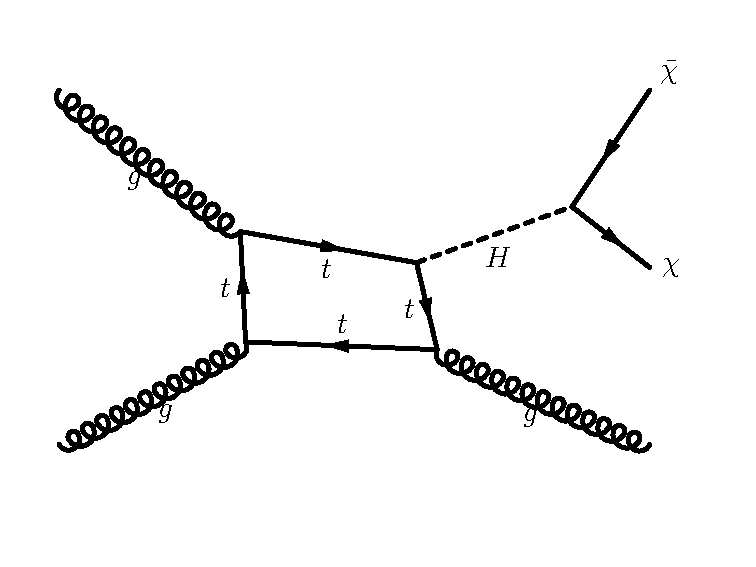
\includegraphics[width=\textwidth]{figures/vbf/diagrams/ggf_hinv.pdf}
            \caption{$gg\rightarrow H(\rightarrow\chi\bar\chi)$+jet(s)}
        \end{subfigure}
        \begin{subfigure}[t]{0.32\textwidth}
            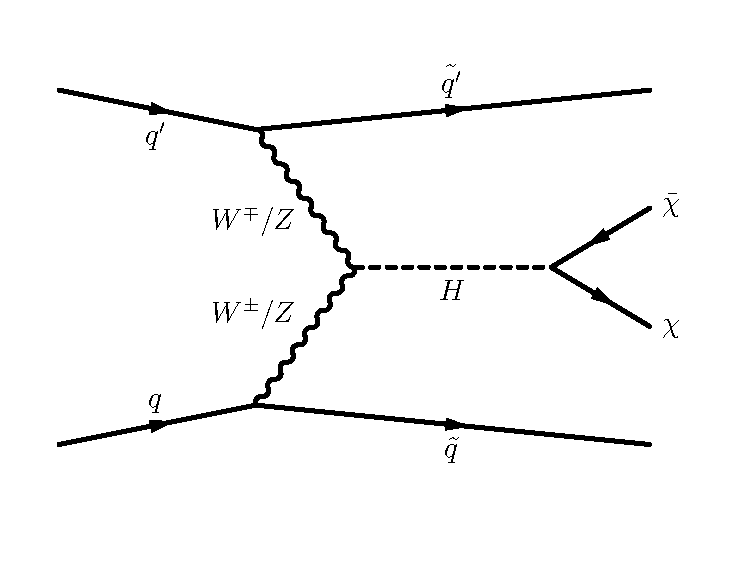
\includegraphics[width=\textwidth]{figures/vbf/diagrams/vbf_hinv.pdf}
            \caption{$qq'\rightarrow H(\rightarrow\chi\bar\chi)$+jet(s)}
        \end{subfigure}
        \begin{subfigure}[t]{0.32\textwidth}
            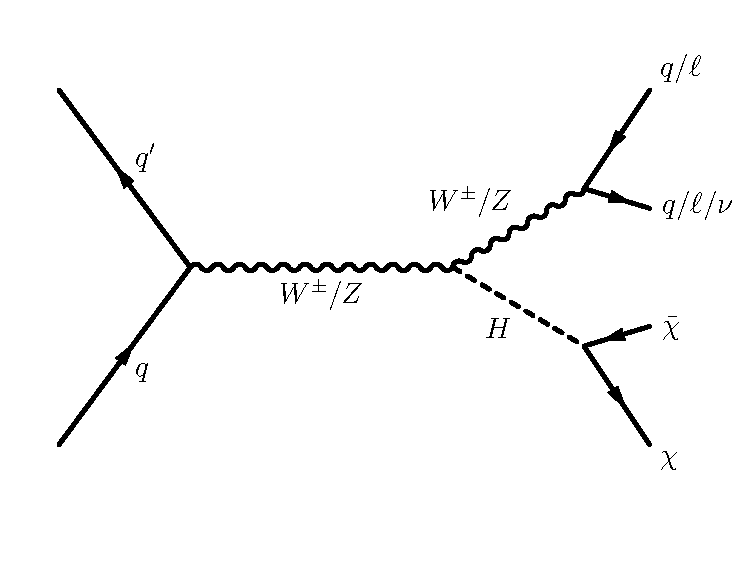
\includegraphics[width=\textwidth]{figures/vbf/diagrams/zh_hinv.pdf}
            \caption{$qq'\rightarrow VH(\rightarrow\chi\bar\chi)$}
        \end{subfigure}
        \caption{Diagrams that contribute to the production of the SM Higgs boson at the LHC, with the subsequent decay to DM candidates.
                 The shown diagrams are all chosen to generate large $\ptmiss$ through the presence of one or more SM particles in the final state.}
        \label{fig:vbf:hdiags}
    \end{center}
\end{figure}

\section{Signal selection}

VBF $\hinv$ events are characterized by large $\ptmiss$ and two jets.
These jets are typically:
\begin{itemize}
    \item Fairly forward in the detector
    \item Far apart from each other in $\eta$
    \item Highly energetic (large $E$, moderate $\pt$)
    \item Close together in $\phi$
\end{itemize}
A candidate VBF $\hinv$ event displaying these properties is shown in a CMS event display in Figure~\ref{fig:vbf:ed}.

\begin{figure}[]
    \begin{center}
        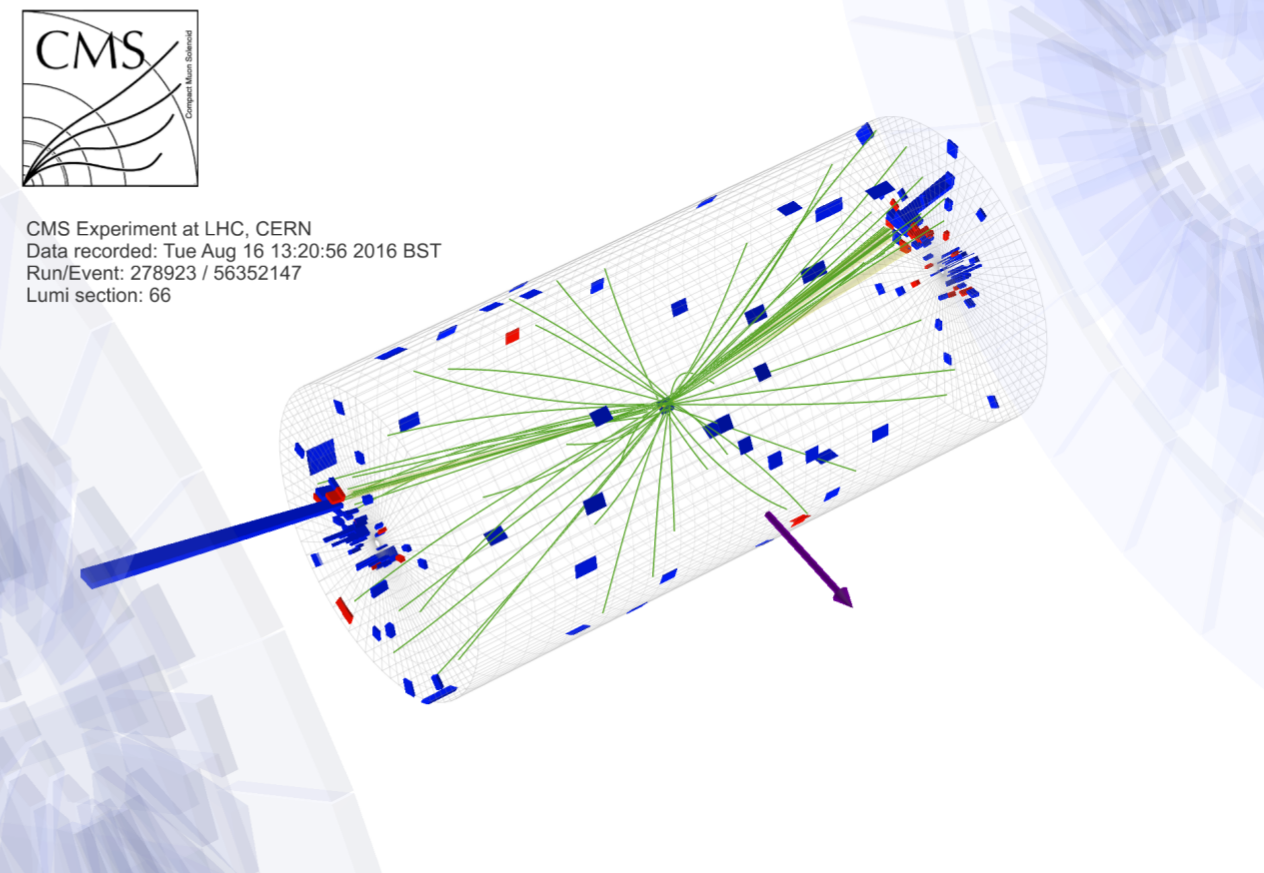
\includegraphics[width=0.8\textwidth]{figures/vbf/misc/event_display.png}
        \caption{Candidate VBF $\hinv$ event with two energetic forward jets ($\pt=180,~107$ GeV) and large $\ptmiss$ ($360$ GeV).
                 Red (blue) towers represent deposits in the hadronic (electromagnetic) calorimeter.
                 Green lines are tracks reconstructed from hits of charged particles in the tracker. 
                 The blue arrow represents the direction and magnitude of the $\ptmiss$.}
        \label{fig:vbf:ed}
    \end{center}
\end{figure}

\subsection{Online trigger selection}
\label{sec:vbf:trig}

The same trigger decisions (L1 and HLT) as described in Section~\ref{sec:mt:trigger} are used to select events in this analysis.
However, the L1 seeds for the 2016 data run were designed with mono-top-like analyses in mind; i.e., searches where the momentum imbalance is created by central objects.
To avoid noise and resolution issues in the forward calorimeters, the L1 seed only considers energy deposits in the region ${|\eta|<3}$. 
Therefore, VBF events in which both jets are in the forward region are not selected.  

This is visible in Figure~\ref{fig:vbf:hlta}, where events are classified based on the location of the two highest-$\pt$ jets.
Events with both jets in the barrel (BB) have a higher efficiency than events with one jet in the forward detector (BF).
Note that events with two forward jets (FF) are not considered at all, as the efficiency for such events is essentially zero. 

\begin{figure}[]
    \begin{center}
        \begin{subfigure}[t]{0.49\textwidth}
            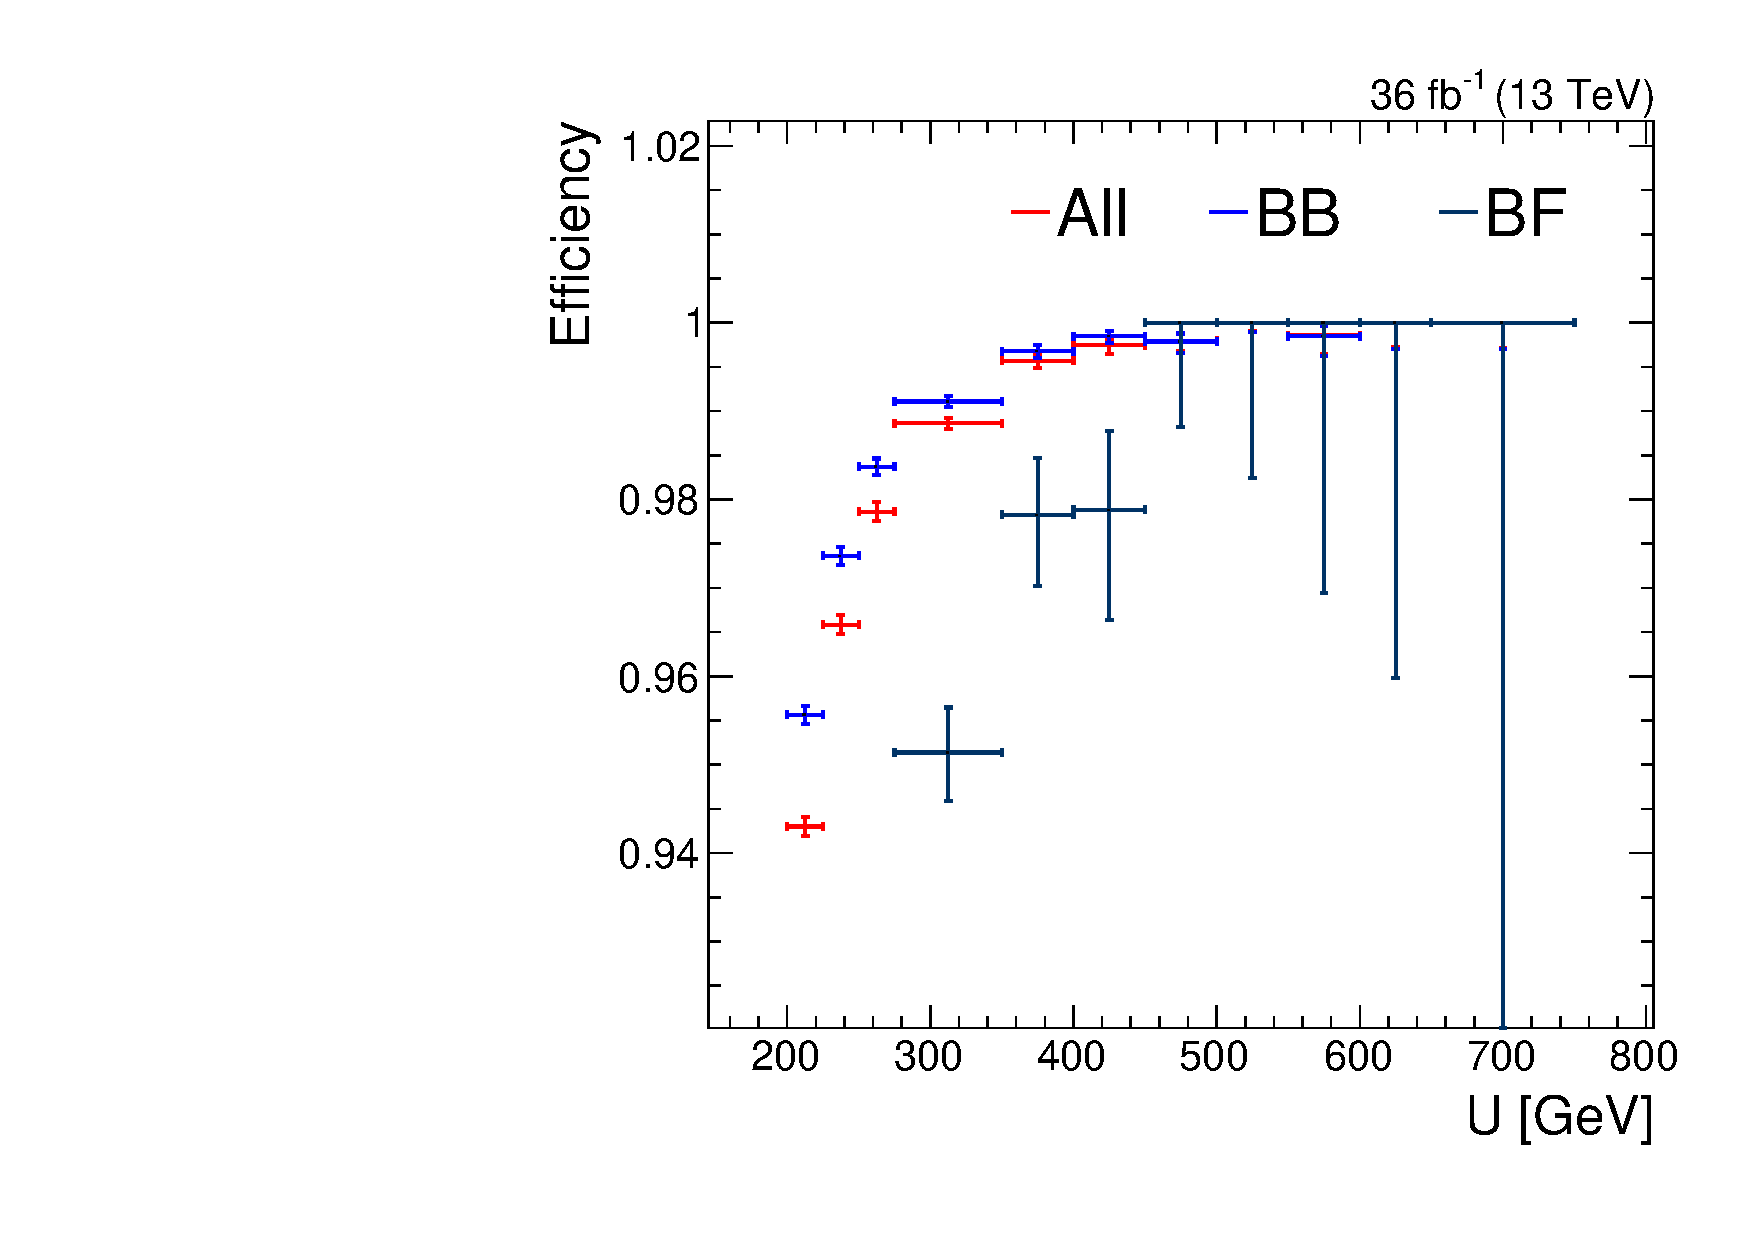
\includegraphics[width=\textwidth]{figures/vbf/triggers/trigeff_nmu1pfUWmag.pdf}
            \caption{Recoil}
            \label{fig:vbf:hlta}
        \end{subfigure}
        \begin{subfigure}[t]{0.49\textwidth}
            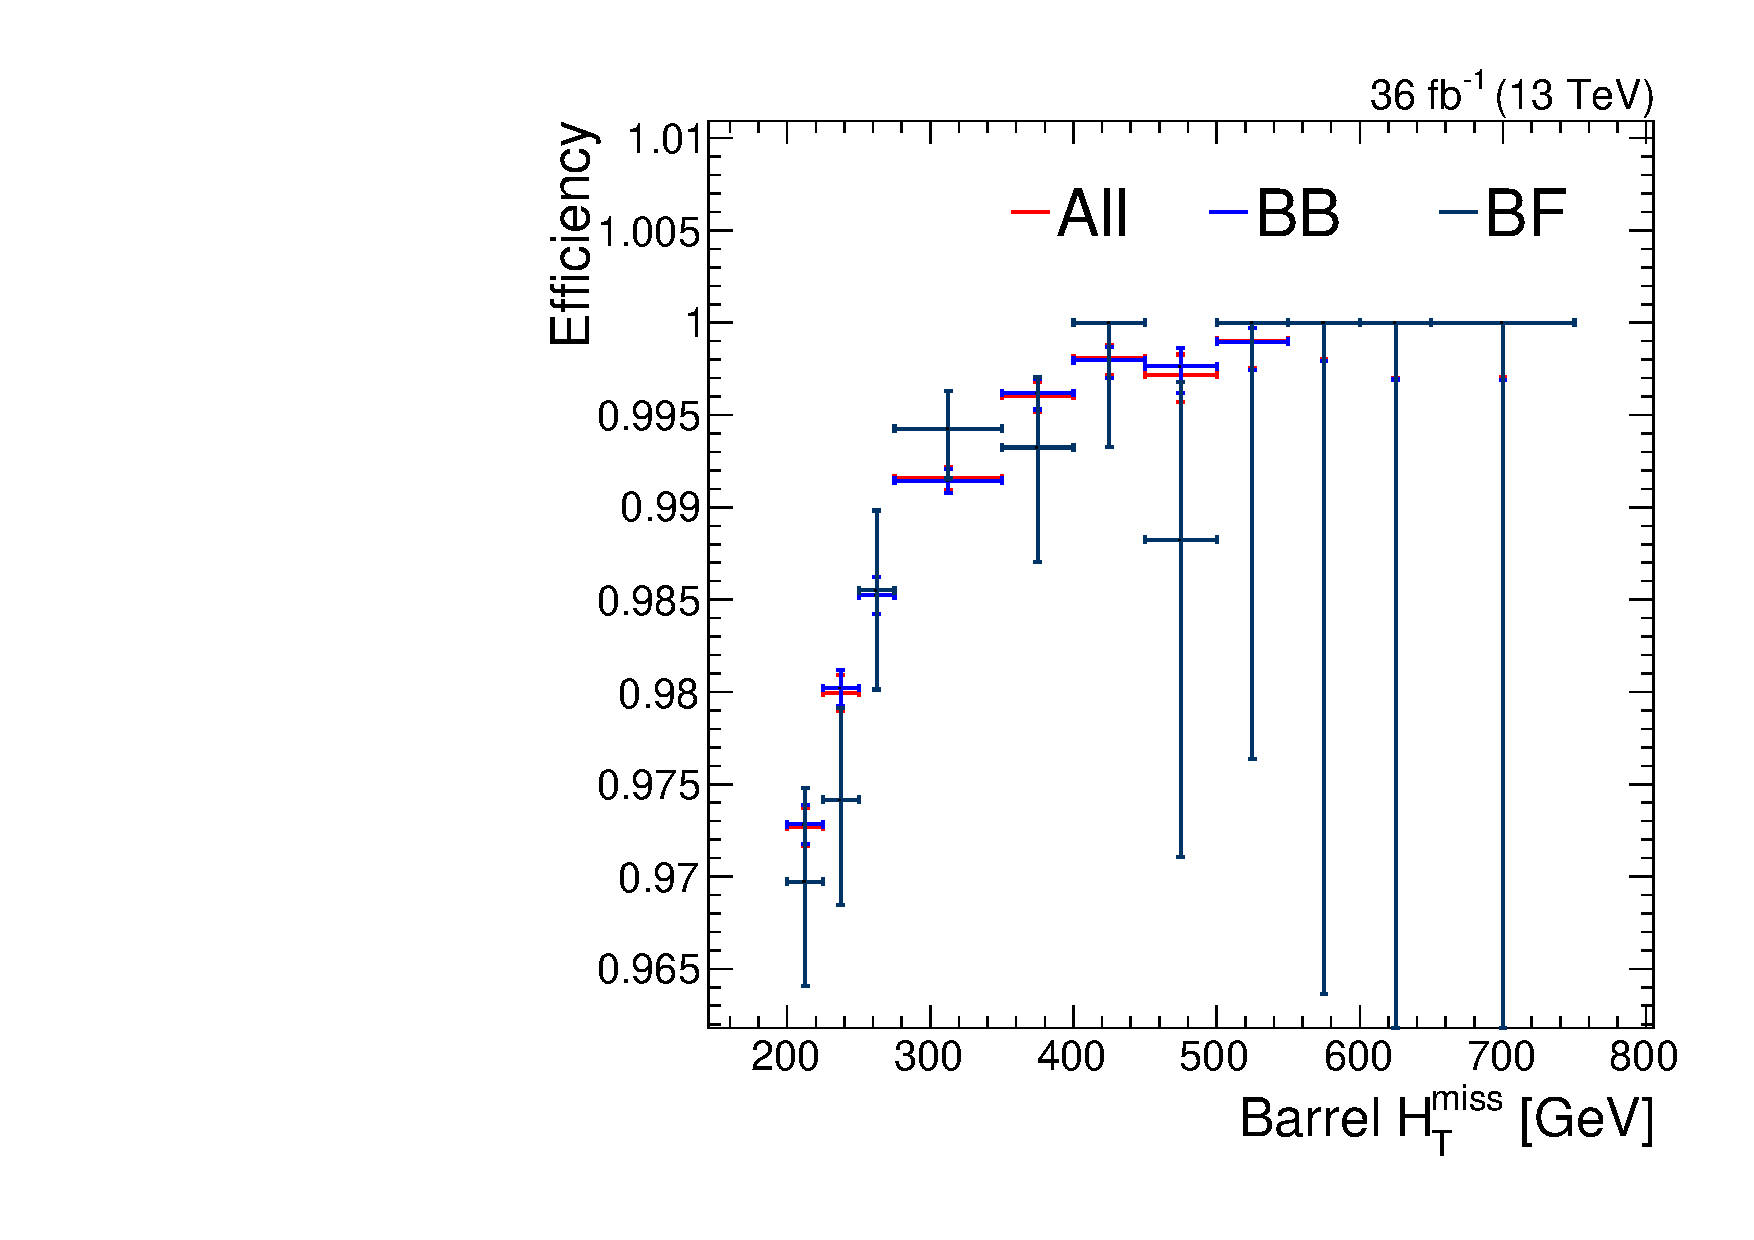
\includegraphics[width=\textwidth]{figures/vbf/triggers/trigeff_nmu1barrelHTMiss.pdf}
            \caption{$H_\mathrm{T,barrel}^\mathrm{miss}$}
            \label{fig:vbf:hltb}
        \end{subfigure}
        \caption{Trigger efficiency of events with a VBF-like topology (two jets with $\pt>80,40$ GeV) as a function of two different observables.
                 Events are split into two categories: those where both jets have $|\eta|<3$ (BB) and those were exactly one jet has $|\eta|>3$ (FF).
                 "All" refers to the sum of these categories.}
        \label{fig:vbf:hlt}
    \end{center}
\end{figure}

The trigger efficiency is truly characterized by the energy deposited in the $|\eta|<3$ region of the detector, and will be dominated in VBF events by the energy of jets.
Accordingly, we define the ``missing barrel hadronic transverse momentum'':
\begin{equation}
    H_\mathrm{T,barrel}^\mathrm{miss} = \left|\left(\sum_{j\in\text{barrel}} \vec{p}_j \right)_\mathrm{T}\right|, \text{ where barrel refers to jets with $|\eta|<3$}
\end{equation}
As shown in Figure~\ref{fig:vbf:hltb}, the three categories (BB, BF, All) have similar behavior as a function of $H_\mathrm{T,barrel}^\mathrm{miss}$.
Therefore, we use this parameterization of the efficiency to correct MC simulation to match data. 

A second L1-related issue that plagues the 2016 dataset is caused by a ``pre-firing'' effect.
When an L1 seed is triggered to accept an event (``L1Accept'' or ``L1A''), the following two bunch crossings (not necessarily corresponding to collisions) are blocked from firing L1As. 
At most, two in four consecutive events can fire L1A (i.e. the sequence L1A, blocked, blocked, L1A).
Figure~\ref{fig:vbf:pre1} is an example of a normal ECAL L1 seed accepting an event and blocking the subsequent bunch crossings.
In what follows, we will refer to the bunch crossing with an interesting collision (i.e. the one we would like the trigger to select) as \bx{0}.

\begin{figure}
    \begin{center}
        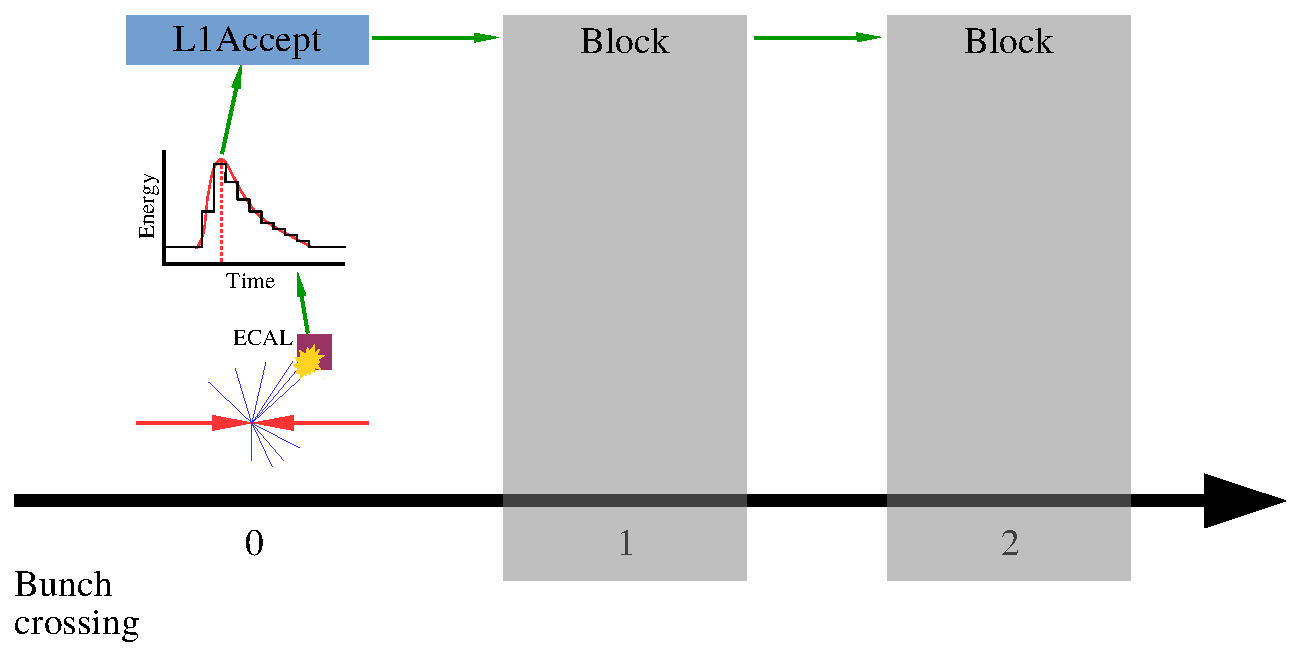
\includegraphics[width=0.8\textwidth,page=1]{figures/vbf/triggers/l1diag.pdf}
        \caption{A normal event in which an ECAL seed triggers the L1A signal. 
                 The subsequent two bunch crossings are blocked. 
                 \bx{0}~refers to the event containing the physics object of interest.
                 Green arrows indicate causality.}
        \label{fig:vbf:pre1}
    \end{center}
\end{figure}

A pre-fire refers to the case in which a malformed detector signal is mis-reconstructed, so that the peak of the pulse appears to have occurred in the previous bunch crossing (\bx{-1}).   
In this particular case, a region of the ECAL ($2.5 < |\eta|<3$) suffered from a loss in transparency due to radiation damage and would produce pulse shapes that are poorly described by the model used to extract the pulse energy and time. 
When this happens, the L1 seeds for ECAL-based signatures (e.g. electron triggers) can fire an L1A for \bx{-1}.
This ECAL L1 seed in \bx{-1}~will zero out the corresponding ECAL clusters in \bx{0} (known as zero suppression), further biasing the event description.
So, we would have an L1A for an arbitrary event (\bx{-1}), and the interesting event (\bx{0}) would be blocked from passing the L1 altogether. 
This is depicted in Figure~\ref{fig:vbf:pre2}.
Typically, \bx{-1}~contains uninteresting physics signatures, and so is not accepted by the HLT.

\begin{figure}
    \begin{center}
        \includegraphics[width=0.8\textwidth,page=2]{figures/vbf/triggers/l1diag.pdf}
        \caption{A pre-fired event in which an ECAL seed triggers the L1A signal for \bx{-1}. 
                 The subsequent two bunch crossings (including the one of interest) are blocked. 
                 \bx{0}~refers to the event containing the physics object of interest.
                 Green arrows indicate causality.}
        \label{fig:vbf:pre2}
    \end{center}
\end{figure}

To measure how often an ECAL energy deposit (typically left by a jet) causes an event to be lost by pre-firing, we need to compute the following efficiency:
\begin{equation}
    \epsilon_\text{pre-fire}(\pt,\eta,\phi) = \frac{N_\text{pre-fire}(\pt,\eta,\phi)}{N_\text{all events}(\pt,\eta,\phi)}
\end{equation}
However, by definition, pre-fired events cannot be recorded, and therefore $N_\text{pre-fire}(\pt,\eta,\phi)$ is difficult to measure.
A very small subset of the recorded dataset ($0.2\%$) consists of ``un-pre-fireable'' events.
These are recorded events (\bx{0}) in which an L1A fired 3 bunch crossings prior (\bx{-3}).
Due to the blocking rules, L1A cannot fire in \bx{-2}~and \bx{-1}.
Even if there is an ECAL seed in \bx{0}~that pre-fires, it will be blocked from firing an L1A, and therefore \bx{0}~is protected.
If some other object in \bx{0}~manages to pass L1 and HLT decisions, then \bx{0}~will be recorded and can be studied.
A schematic of such events is shown in Figure~\ref{fig:vbf:pre3}.

\begin{figure}
    \begin{center}
        \includegraphics[width=0.8\textwidth,page=3]{figures/vbf/triggers/l1diag.pdf}
        \caption{An un-pre-fireable event in which \bx{-3}~protects \bx{0}~from being pre-fired. 
                 Green arrows indicate causality.}
        \label{fig:vbf:pre3}
    \end{center}
\end{figure}

The L1 trigger system records trigger primitive (TP) information (4-vectors of physics objects considered in an L1 selection) for \bx{-1}~if \bx{0}~is triggered.
This means we can identify the cases in which a physics object in \bx{0}~coincides with a TP in \bx{-1}, indicating a pre-fire. 
Therefore (using the bunch crossing numbering in Figure~\ref{fig:vbf:pre3}), we re-define the efficiency:
\begin{equation}
    \epsilon_\text{pre-fire}(\pt,\eta,\phi) = \frac{N_\text{pre-fire \bx{0}|\bx{-3}}(\pt,\eta,\phi)}{N_\text{\bx{0}|\bx{-3}}(\pt,\eta,\phi)}
\end{equation}
By definition, all events in this ratio will be recorded. 
Figure~\ref{fig:vbf:pre_eff2_etaphi} shows this efficiency as a function of jet location. 
We observe there is a ``hot'' ECAL tower near the location $\eta=-2.8$ and $\phi=2$.
Not only does this tower fire very frequently (leading to many particles, leading to many jets), but it almost always pre-fires.
To first order, events with a jet in this crystal should be rejected.
Beyond this, there is very little localization in the pre-fire probability (besides restriction to the ECAL endcap). 

\begin{figure}[]
    \begin{center}
        \begin{subfigure}[t]{0.49\textwidth}
            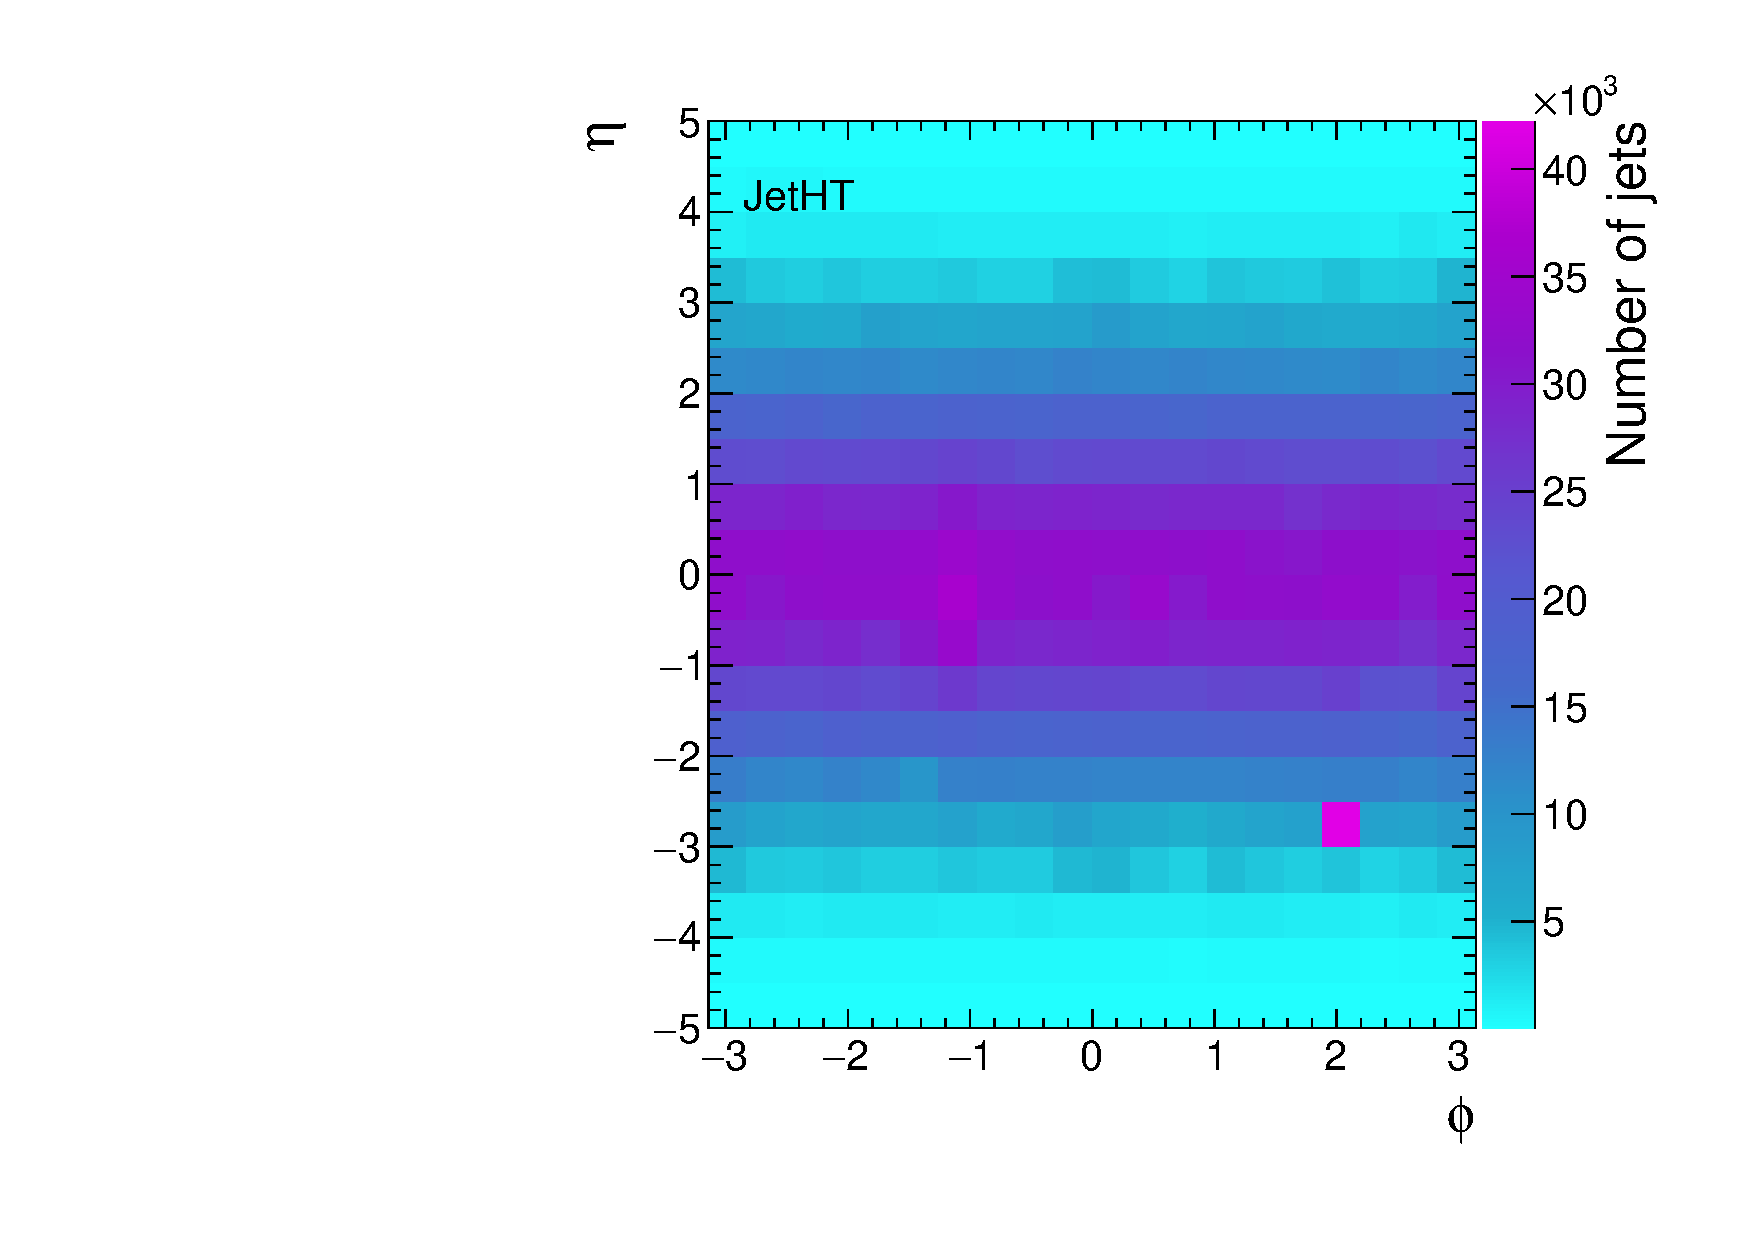
\includegraphics[width=\textwidth]{figures/vbf/triggers/JetHT_inclusive_egiso_etaphi_den.pdf}
            \caption{Number of jets}
        \end{subfigure}
        \begin{subfigure}[t]{0.49\textwidth}
            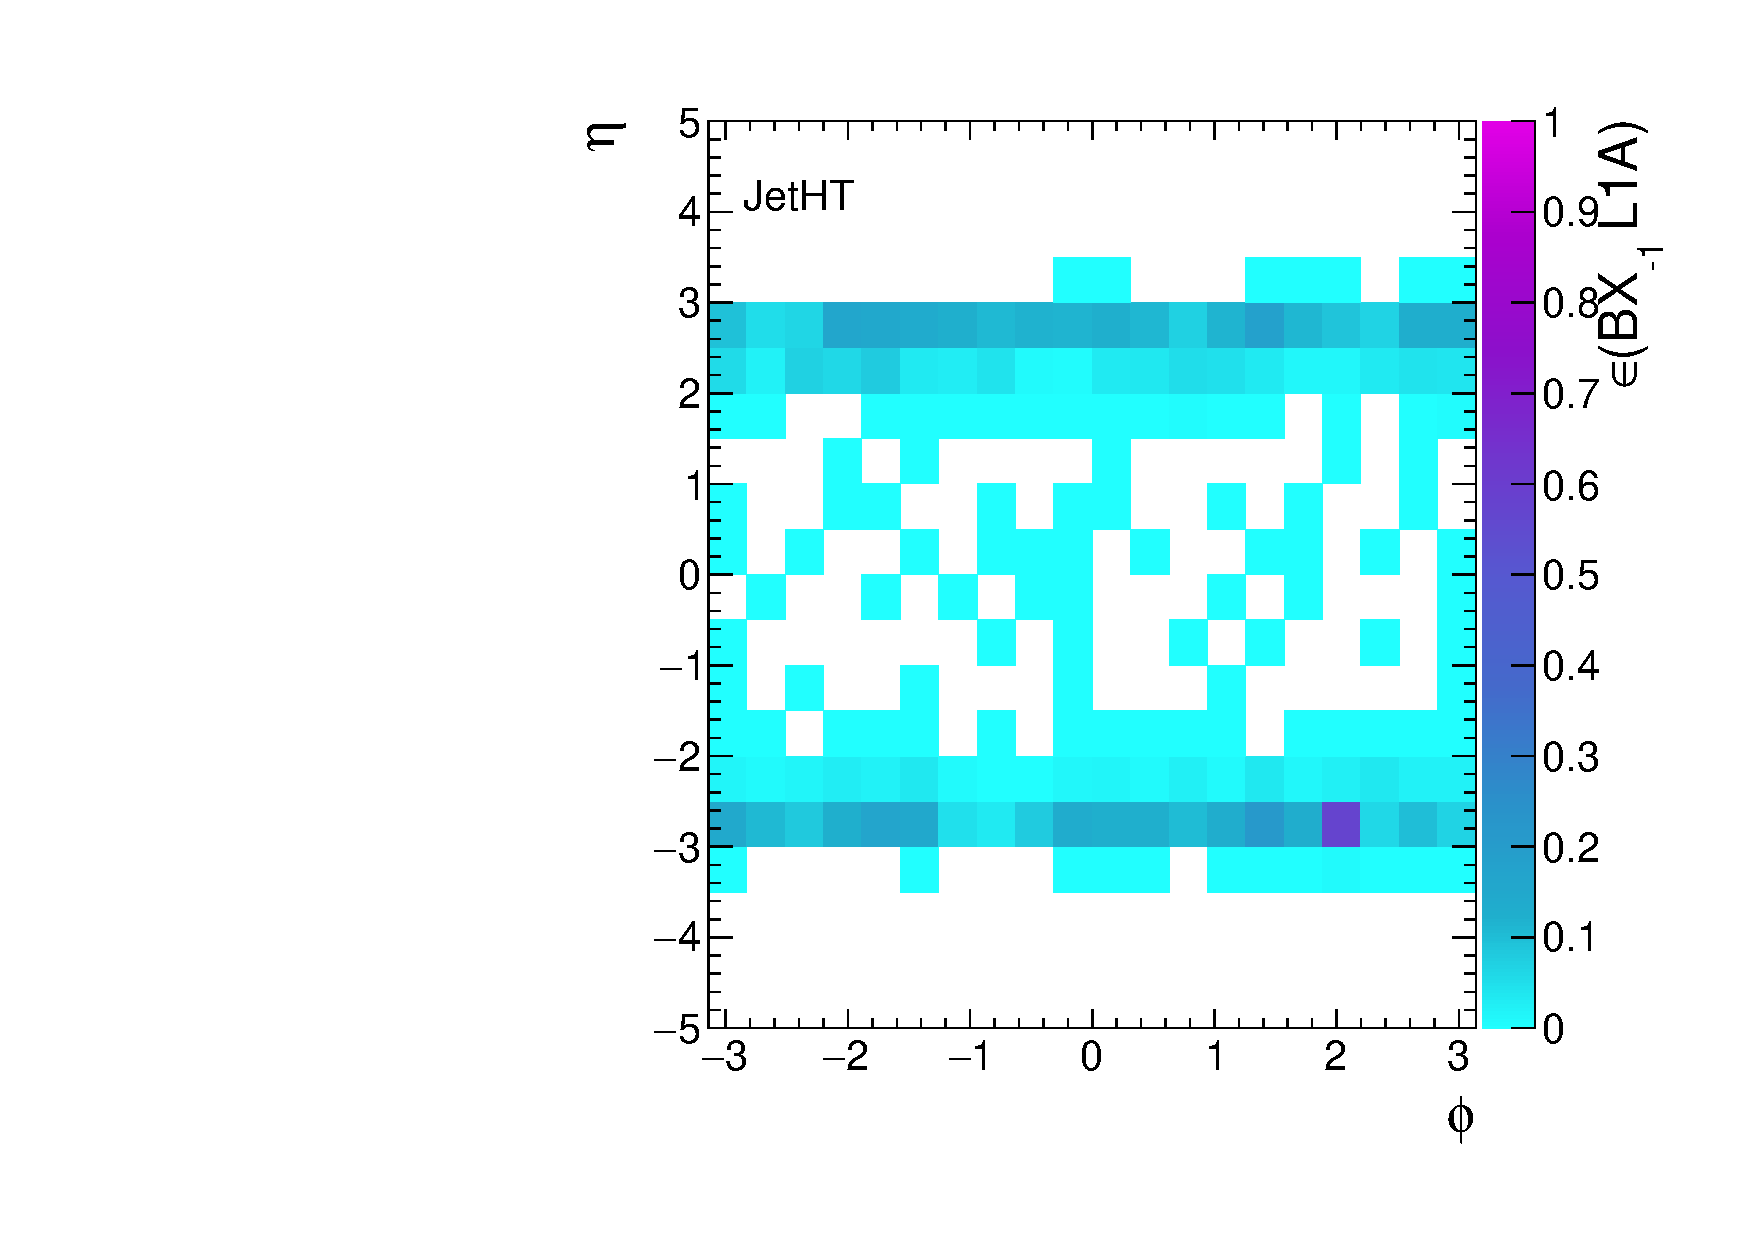
\includegraphics[width=\textwidth]{figures/vbf/triggers/JetHT_inclusive_egiso_etaphi_ratio.pdf}
            \caption{Pre-fire probability}
        \end{subfigure}
        \caption{Distribution of jets and pre-fire events as a function of the jet location in the detector.
                 Note the spike near $(\eta,\phi) = (-2.8,2)$. }
        \label{fig:vbf:pre_eff2_etaphi}
    \end{center}
\end{figure}

In Figure~\ref{fig:vbf:pre_eff1} we see $\epsilon_\text{pre-fire}$ as a function of $\pt$ in a restricted $\eta$ range.
Firstly, we observe that $\epsilon_\text{pre-fire}$ increases as a function of $\pt$, and the turn-on is sharper as a function of EM $\pt$. 
This is explained by the mechanism of the pre-fire: the individual ECAL trigger seeds have a threshold of 30 GeV.
The higher the jet $\pt$, the higher the probability of the jet depositing $30$ GeV of EM energy in a localized area, setting off an L1 seed. 
Secondly, we observe a strong dependence on the reference triggers used to select $\bx{0}$.
For example, jet-based triggers (JetHT) lead to a much higher efficiency than $\ptmiss$-based triggers (MET).  
This is a consequence of zero suppression biasing the \bx{0}~triggers, as shown diagrammatically in Figure~\ref{fig:vbf:pre_diag}.
Muon-based triggers (SingleMuon) are largely unaffected by the ECAL system, and therefore this measurement of $\epsilon_\text{pre-fire}$ is the least biased.  

\begin{figure}[]
    \begin{center}
        \begin{subfigure}[t]{0.49\textwidth}
            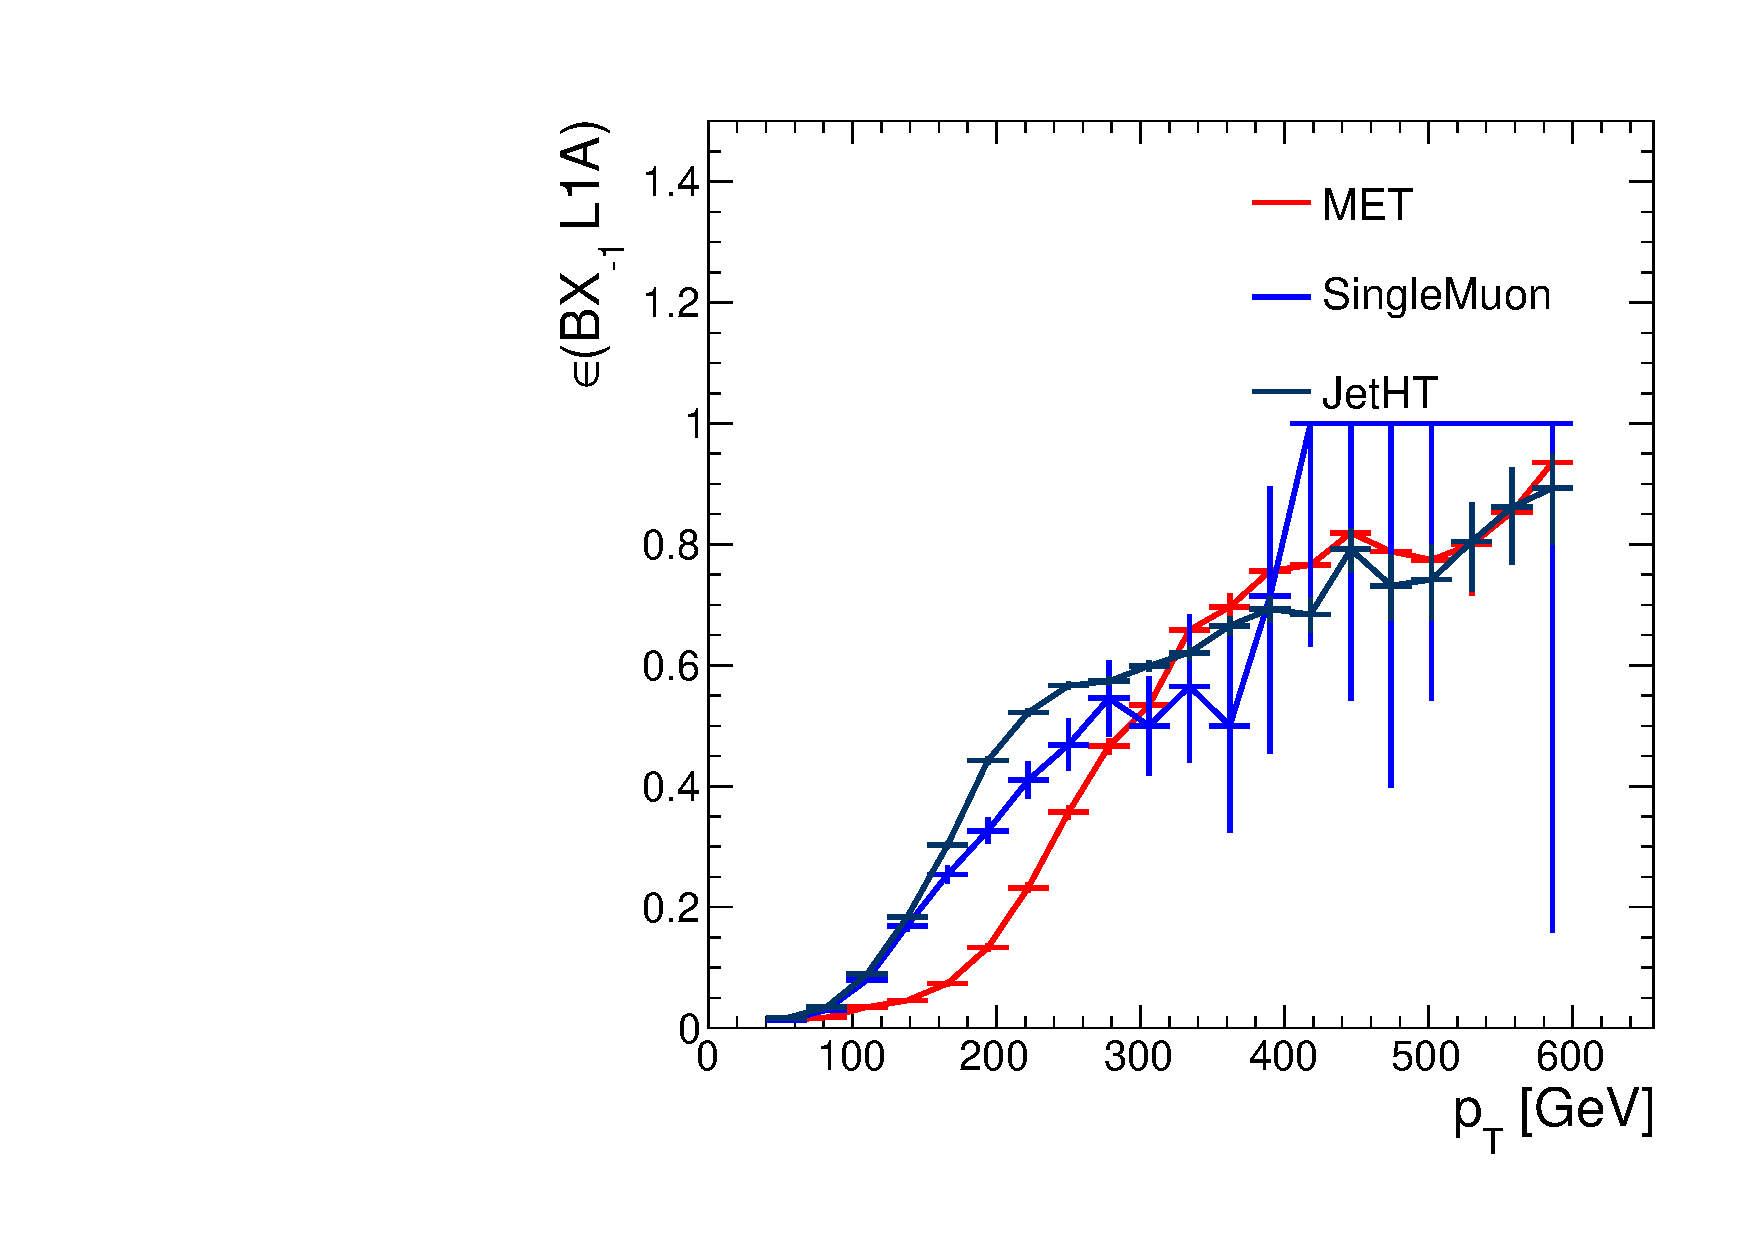
\includegraphics[width=\textwidth]{figures/vbf/triggers/oned_jotPt_finor_ratio.pdf}
            \caption{$\pt$}
        \end{subfigure}
        \begin{subfigure}[t]{0.49\textwidth}
            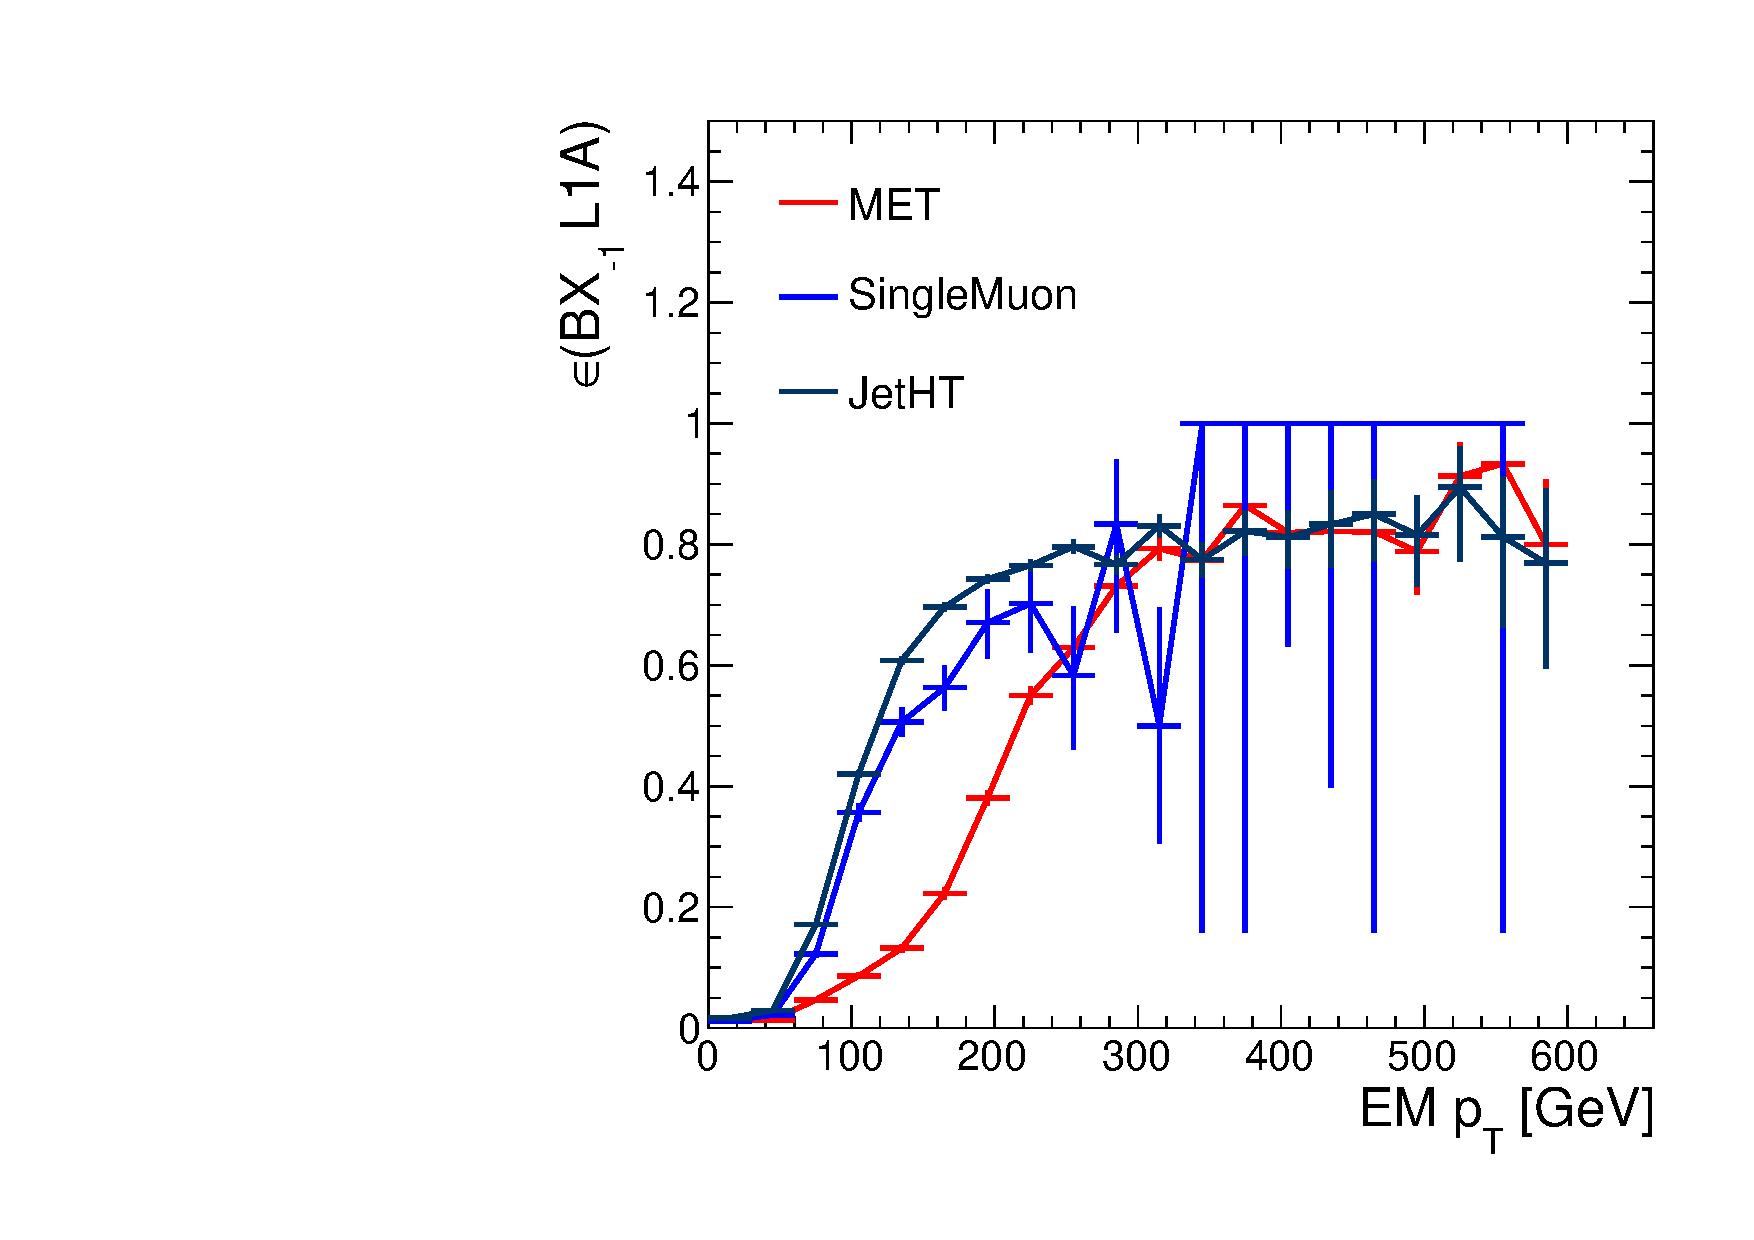
\includegraphics[width=\textwidth]{figures/vbf/triggers/oned_jotEMPt_finor_ratio.pdf}
            \caption{$\pt \times E_\mathrm{ECAL}/E_\mathrm{total}$}
        \end{subfigure}
        \caption{Probability that a given jet with $2.25<|\eta|<3$ causes a pre-fire in the L1 trigger due to ECAL mistiming.
                 Two parameterizations are used: jet $\pt$ and EM $\pt$.
                 The three curves refer to which set of triggers are used to select $\bx{0}$.}
        \label{fig:vbf:pre_eff1}
    \end{center}
\end{figure}

\begin{figure}[]
    \begin{center}
        \begin{subfigure}[t]{0.49\textwidth}
            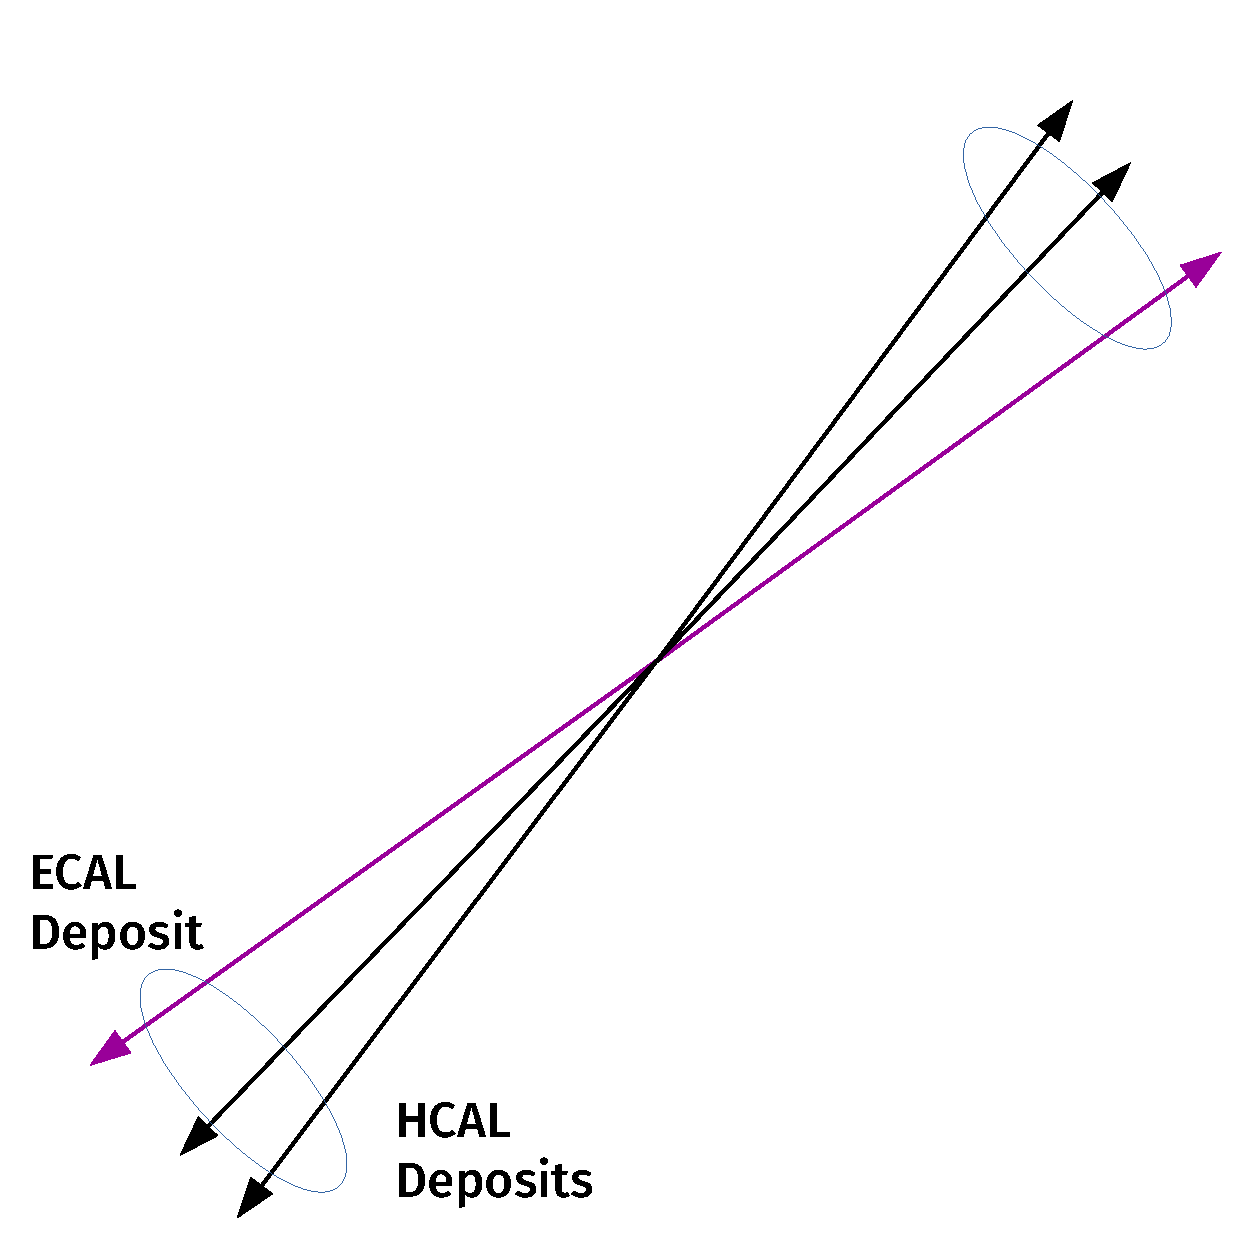
\includegraphics[width=0.49\textwidth]{figures/vbf/triggers/normal_dijet.pdf}
            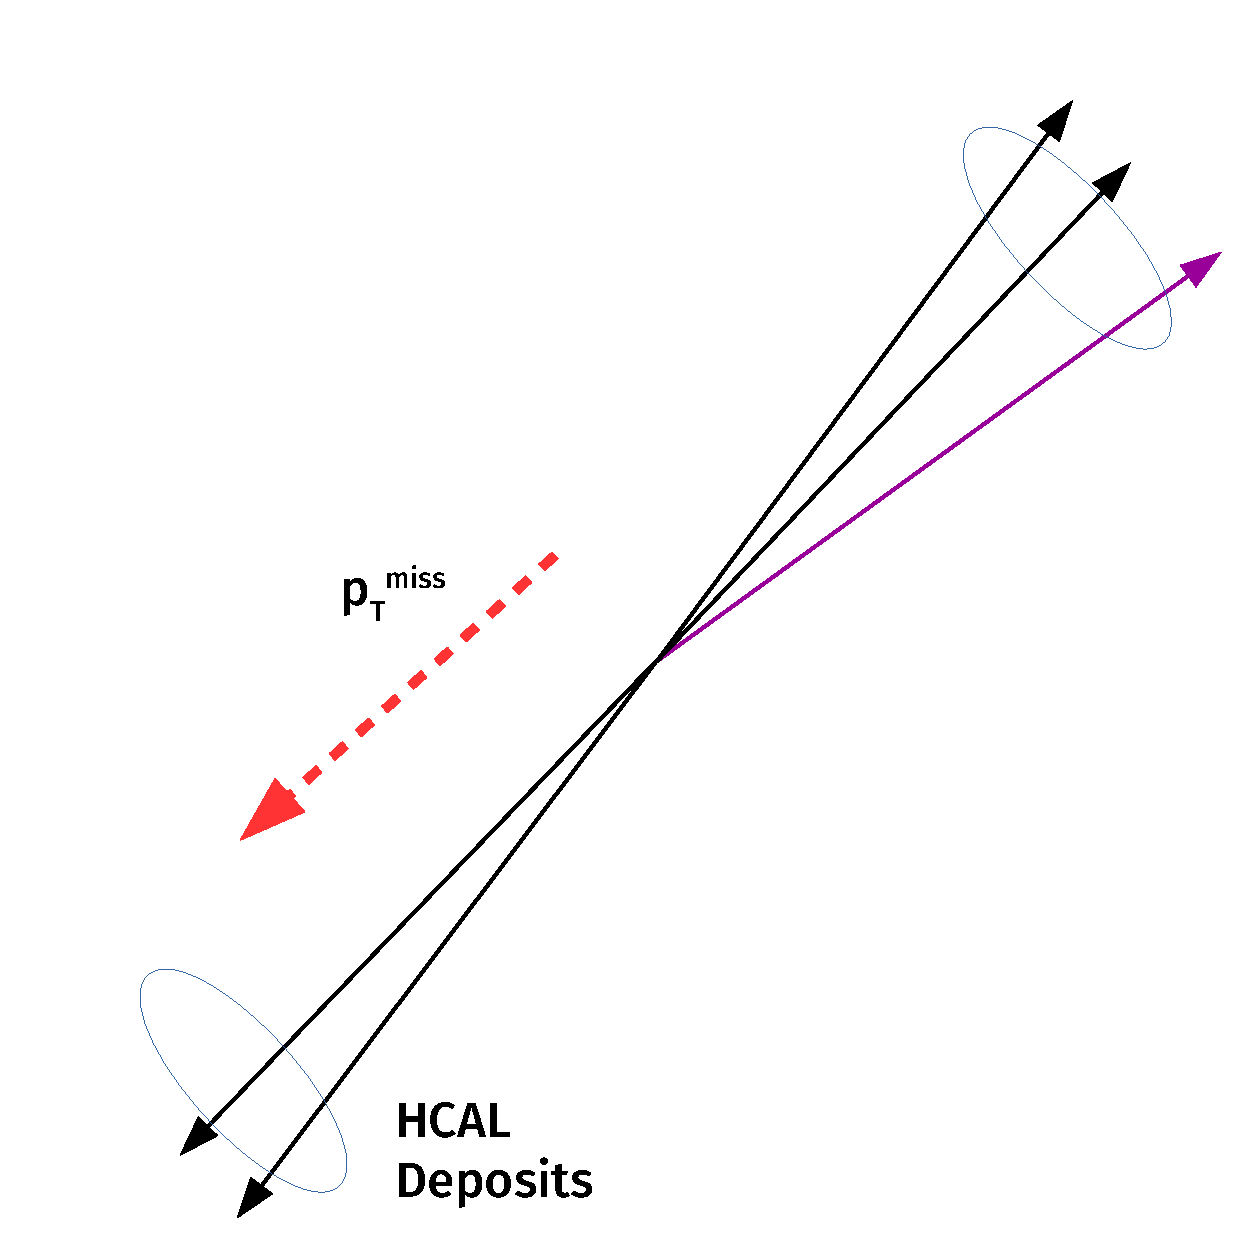
\includegraphics[width=0.49\textwidth]{figures/vbf/triggers/prefire_dijet.pdf}
            \caption{Dijet event}
        \end{subfigure}
        \begin{subfigure}[t]{0.49\textwidth}
            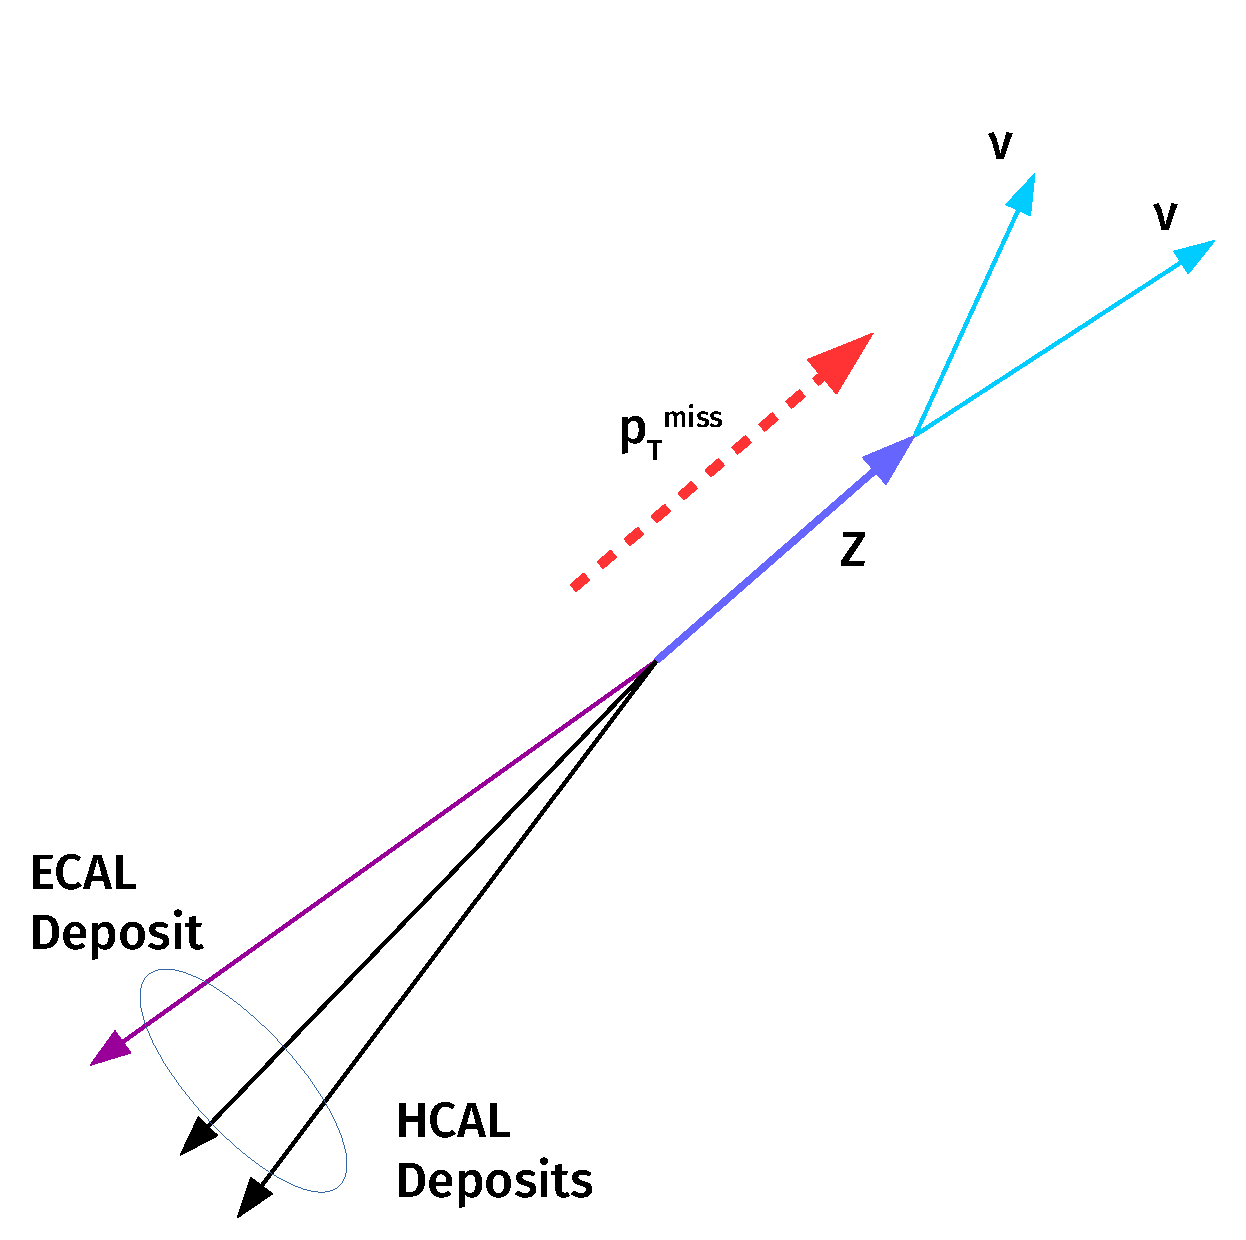
\includegraphics[width=0.49\textwidth]{figures/vbf/triggers/normal_z.pdf}
            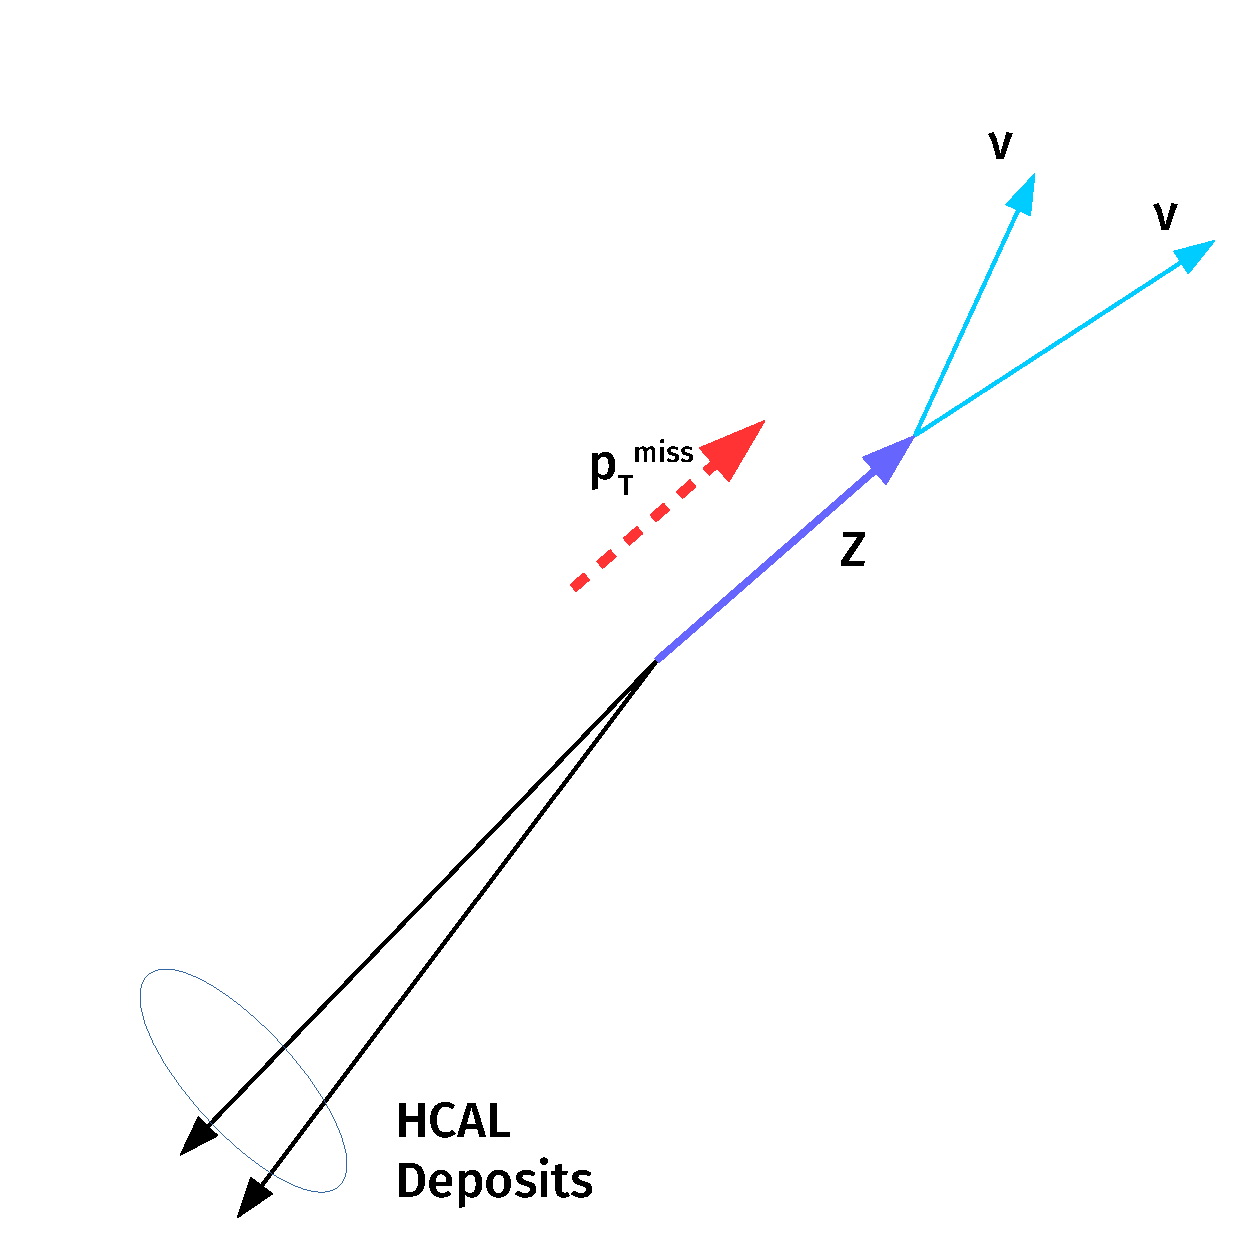
\includegraphics[width=0.49\textwidth]{figures/vbf/triggers/prefire_z.pdf}
            \caption{$Z\rightarrow\nu\nu$ event}
        \end{subfigure}
        \caption{How zero suppression in the ECAL due to pre-firing can bias certain events.
                 Subfigure (a) shows a dijet event, in which the loss of an ECAL deposit reduces the total $H_\mathrm{T}$ of the event, thereby lowering the probability of a jet-based trigger to fire.
                 Subfigure (b) shows a $Z\rightarrow\nu\nu$ event, in which the loss of an ECAL deposit reduces the total $\ptmiss$ of the event.}
        \label{fig:vbf:pre_diag}
    \end{center}
\end{figure}

The probability of at least one jet pre-firing in an event is:
\begin{equation}
    \epsilon_\text{pre-fire}^\text{event} = 1 - \prod_{j\in\text{jets}}  \left(1-\epsilon_\text{pre-fire}(\pt^j,\eta^j)\right)
\end{equation}
The $\phi$-dependence has been dropped, since it is clear from Figure~\ref{fig:vbf:pre_eff2_etaphi} that the effect can be averaged over $\phi$ (once the spike is removed). 
Figure~\ref{fig:vbf:pre_eff2_pteta} shows $\epsilon_\text{pre-fire}(\pt,\eta)$ using muon-triggered and jet-triggered events.
In the former case, statistical fluctuations make the region with $\pt>250$ GeV unusable.
Fortunately, this is the region in which the trigger bias is smallest, and so we switch to the jet triggered measurement above this threshold.
A 20\% uncertainty is assessed on the efficiency, which is derived from the difference between the SingleMuon and JetHT measurements. 

\begin{figure}[]
    \begin{center}
        \begin{subfigure}[t]{0.49\textwidth}
            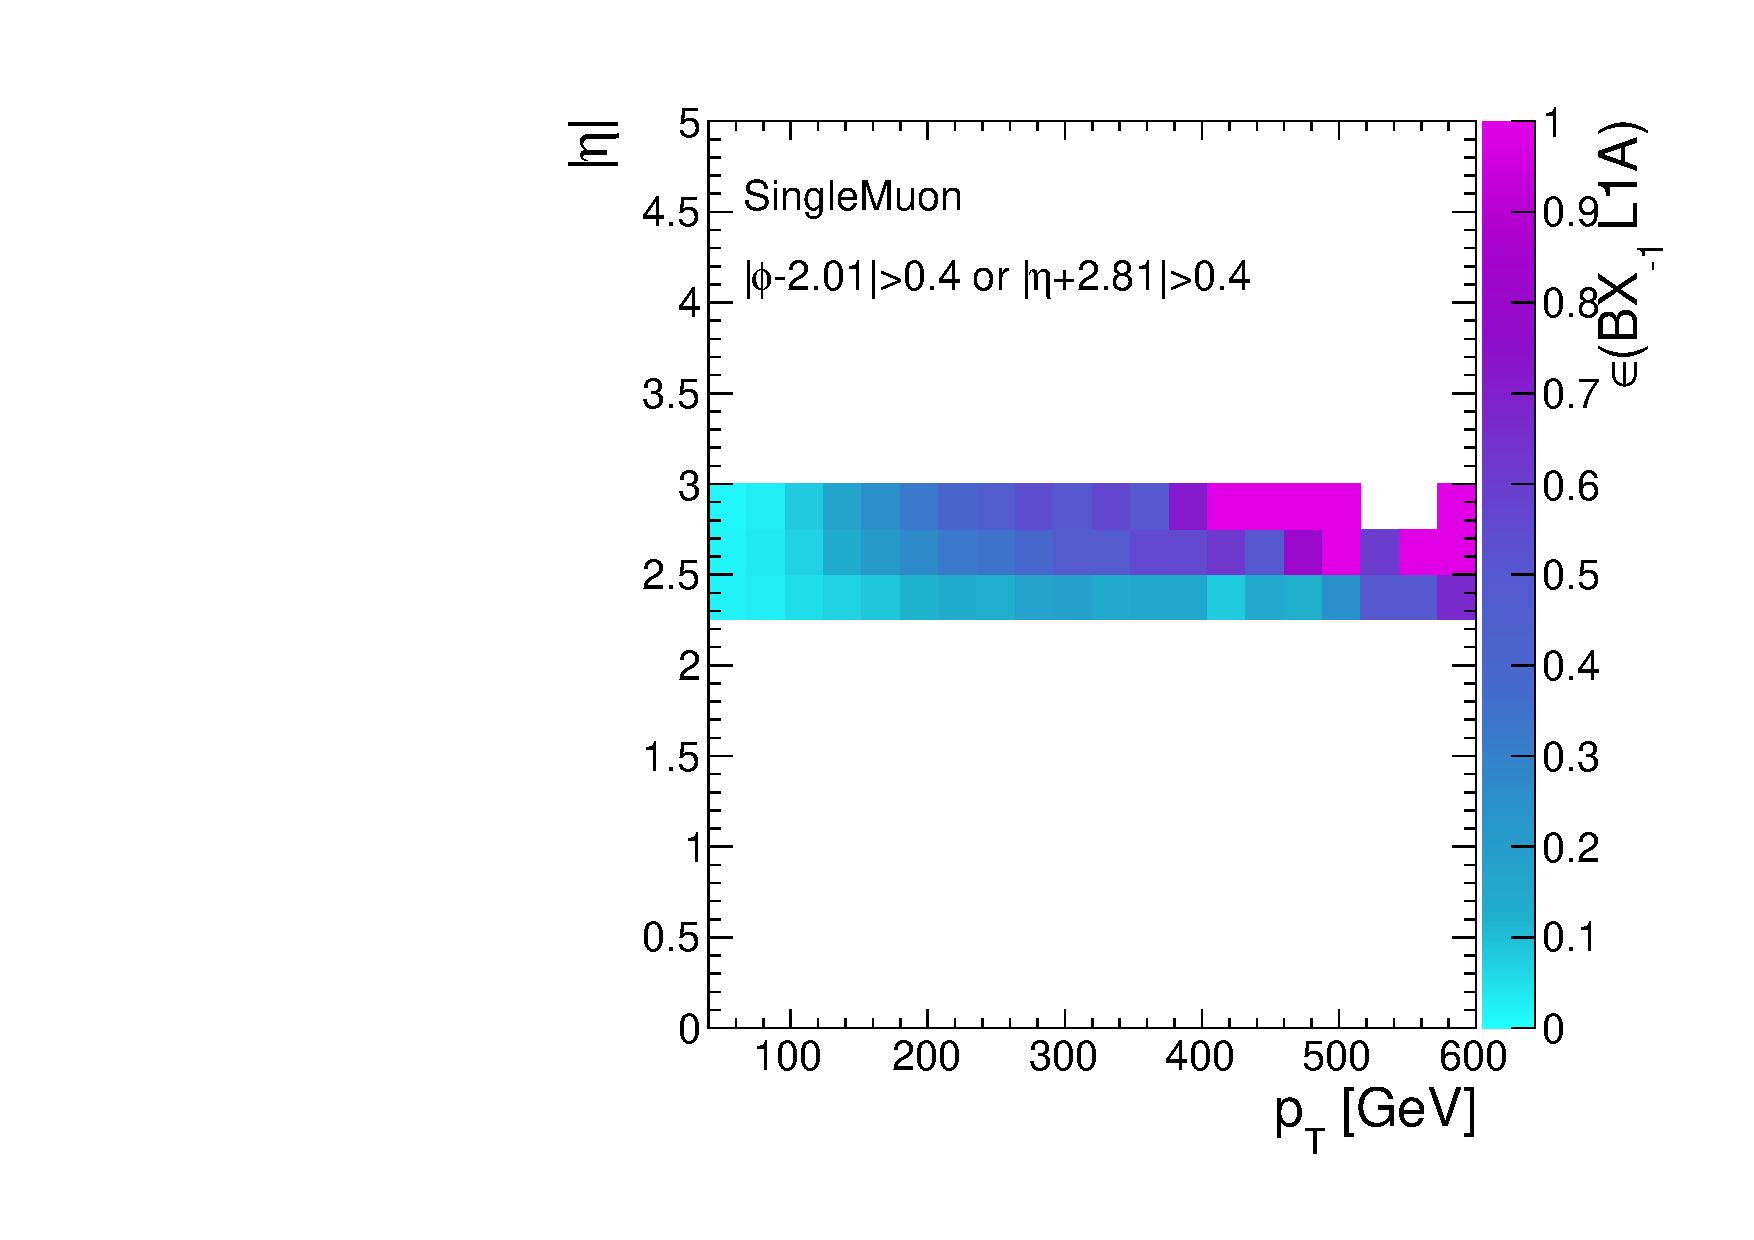
\includegraphics[width=\textwidth]{figures/vbf/triggers/SingleMuon_spike_finor_pteta_ratio.pdf}
            \caption{Muon-triggered}
        \end{subfigure}
        \begin{subfigure}[t]{0.49\textwidth}
            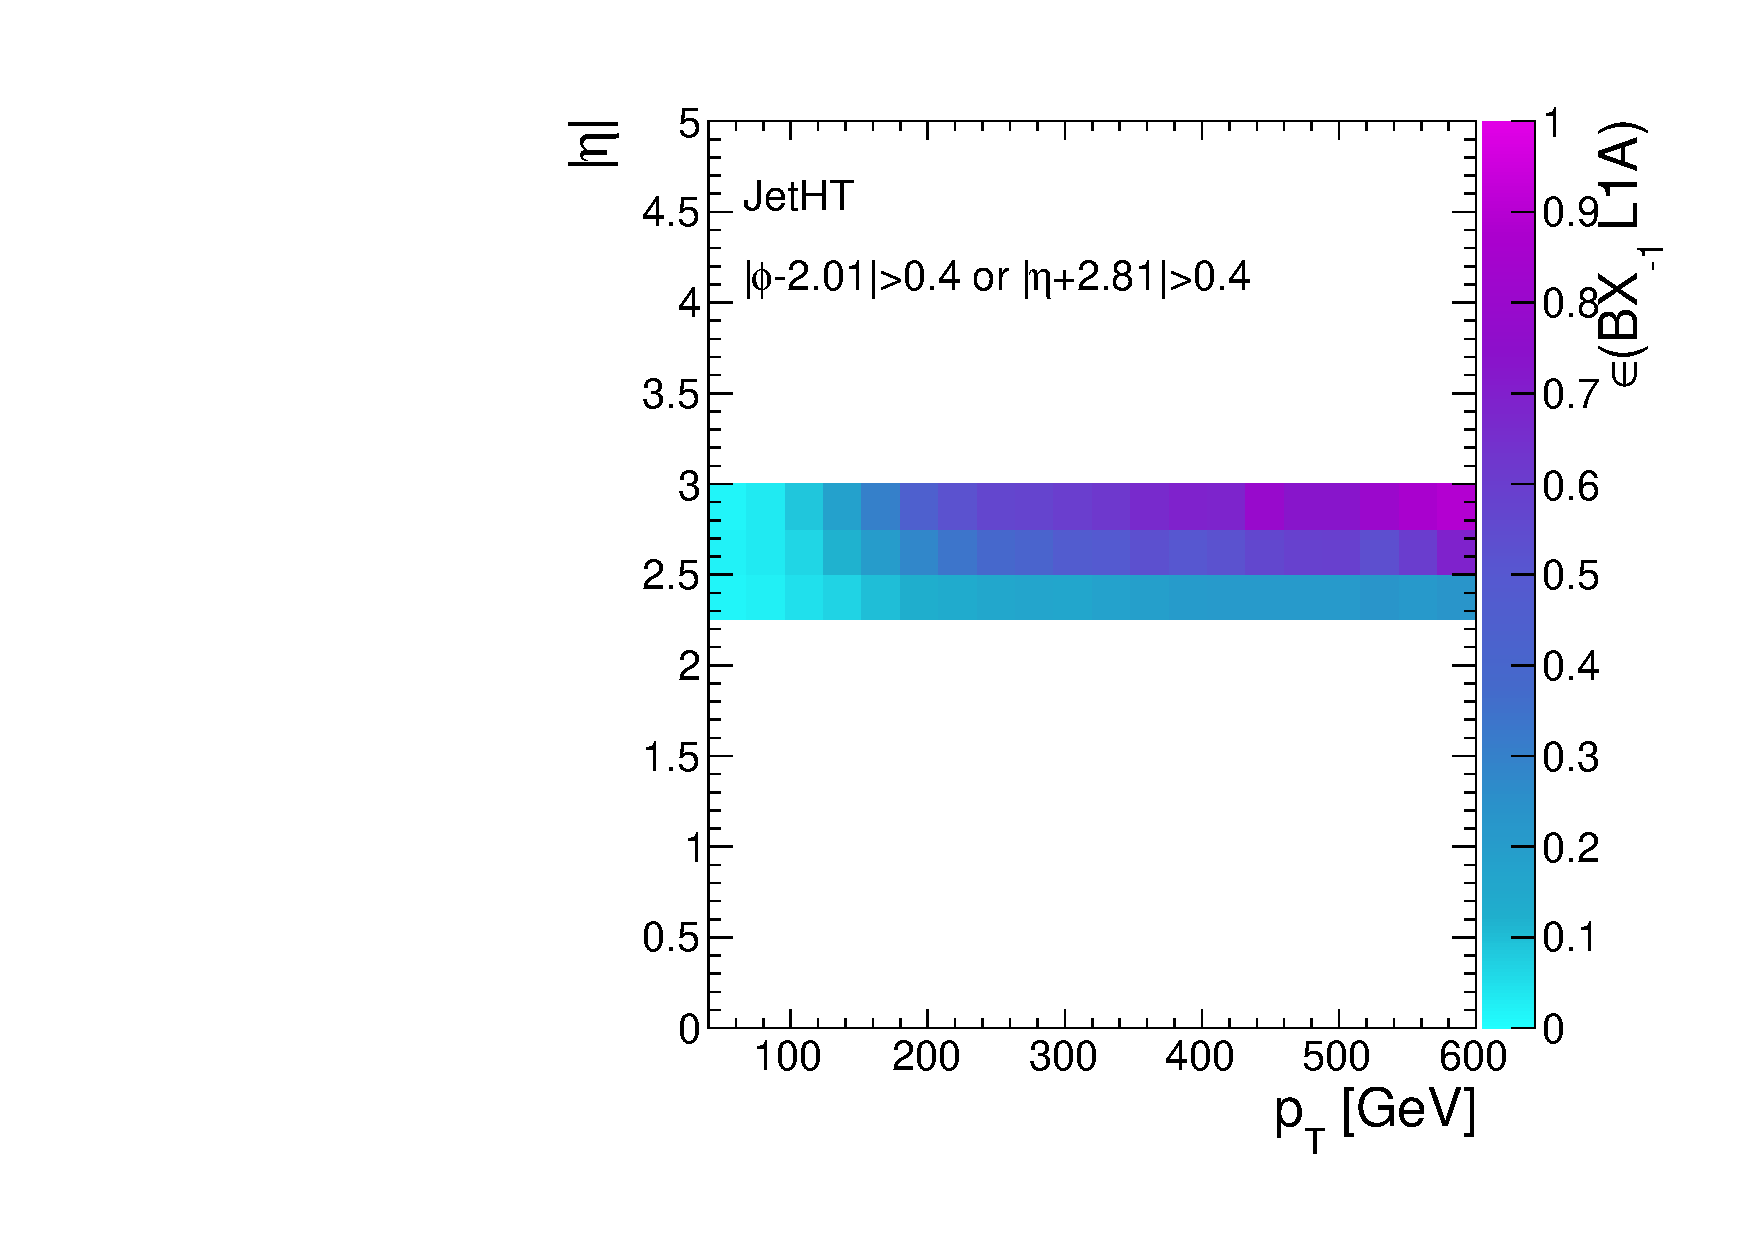
\includegraphics[width=\textwidth]{figures/vbf/triggers/JetHT_spike_finor_pteta_ratio.pdf}
            \caption{Jet-triggered}
        \end{subfigure}
        \caption{$\epsilon_\text{pre-fire}(\pt,\eta)$ with two different sets of reference triggers used to select \bx{0}.}
        \label{fig:vbf:pre_eff2_pteta}
    \end{center}
\end{figure}

\subsection{EW and QCD production of electroweak bosons}

The primary backgrounds to the VBF production of invisibly-decaying Higgs bosons are $Z(\rightarrow\nu\nu)$+2 jet and $W(\rightarrow\ell\nu)$+2 jet production.
At leading order, the relevant Feynman diagrams are either of the order $\alpha_\mathrm{EW}^2 \alpha_\mathrm{QCD}^4$ or $\alpha_\mathrm{EW}^6$. 
We refer to the former as the QCD production mode and the latter as the EW mode. 
Examples Feynman diagrams are shown in Figure~\ref{fig:vbf:ewqcd}.
The EW mode is essentially vector boson fusion, and so the terms EW and VBF will be used interchangeably. 


\begin{figure}[]
    \begin{center}
        \begin{subfigure}[t]{0.49\textwidth}
            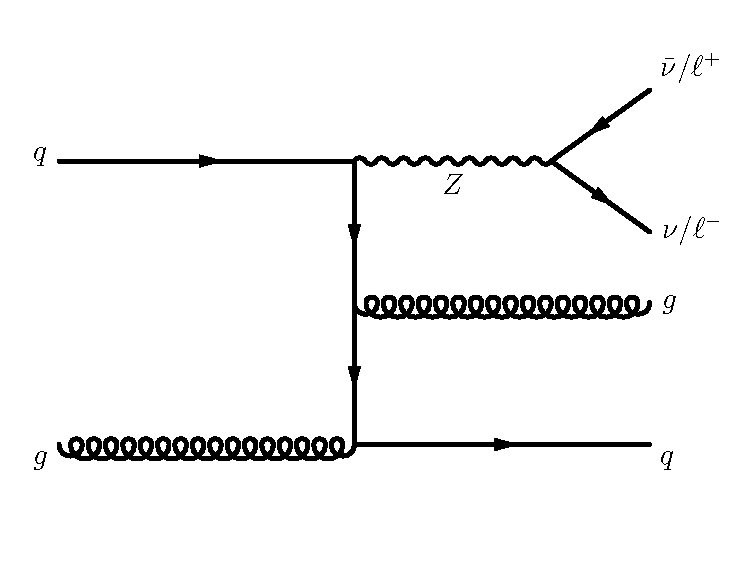
\includegraphics[width=\textwidth]{figures/vbf/diagrams/qcd_z.pdf}
            \caption{QCD}
        \end{subfigure}
        \begin{subfigure}[t]{0.49\textwidth}
            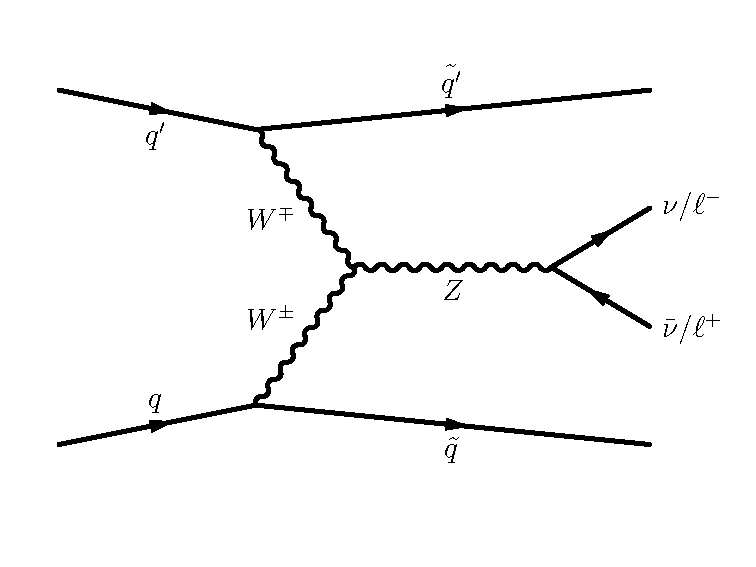
\includegraphics[width=\textwidth]{figures/vbf/diagrams/vbf_z.pdf}
            \caption{EW/VBF}
        \end{subfigure}
        \caption{Examples of the two modes of producing $Z$ bosons in association with 2 jets.
                 Similar diagrams exist for $W$ boson production.}
        \label{fig:vbf:ewqcd}
    \end{center}
\end{figure}

As the vector boson is not directly detectable, the only experimental signatures are the jets.
The jet kinematics are sensitive to the production mode (vector boson fusion vs QCD), as well as the spin of the produced boson.
Some conclusions can be drawn from the kinematic distributions (Figure~\ref{fig:vbf:jetkins}):
\begin{enumerate}
    \item The yield ($\sigma\times A$) of the three VBF processes are relatively close in the relevant phase space (assuming $\mathcal{B}(\hinv)=1$), but the QCD processes are 1-2 orders of magnitude higher.
    \item The jet $\pt$ and $\ptmiss$ distributions in the signal are comparable to or softer than the background processes. 
          This is in contrast to other DM searches, in which the signal $\ptmiss$ distribution is much harder than SM predictions.
    \item VBF $\hinv$ produces fewer jets than SM processes.
    \item VBF $\hinv$ produces relatively forward jets. QCD $V$+jets produces mostly central jets. VBF $V$+jets produces jets that are somewhere between these distributions. 
\end{enumerate}

\begin{figure}[]
    \begin{center}
        \begin{subfigure}[t]{0.32\textwidth}
            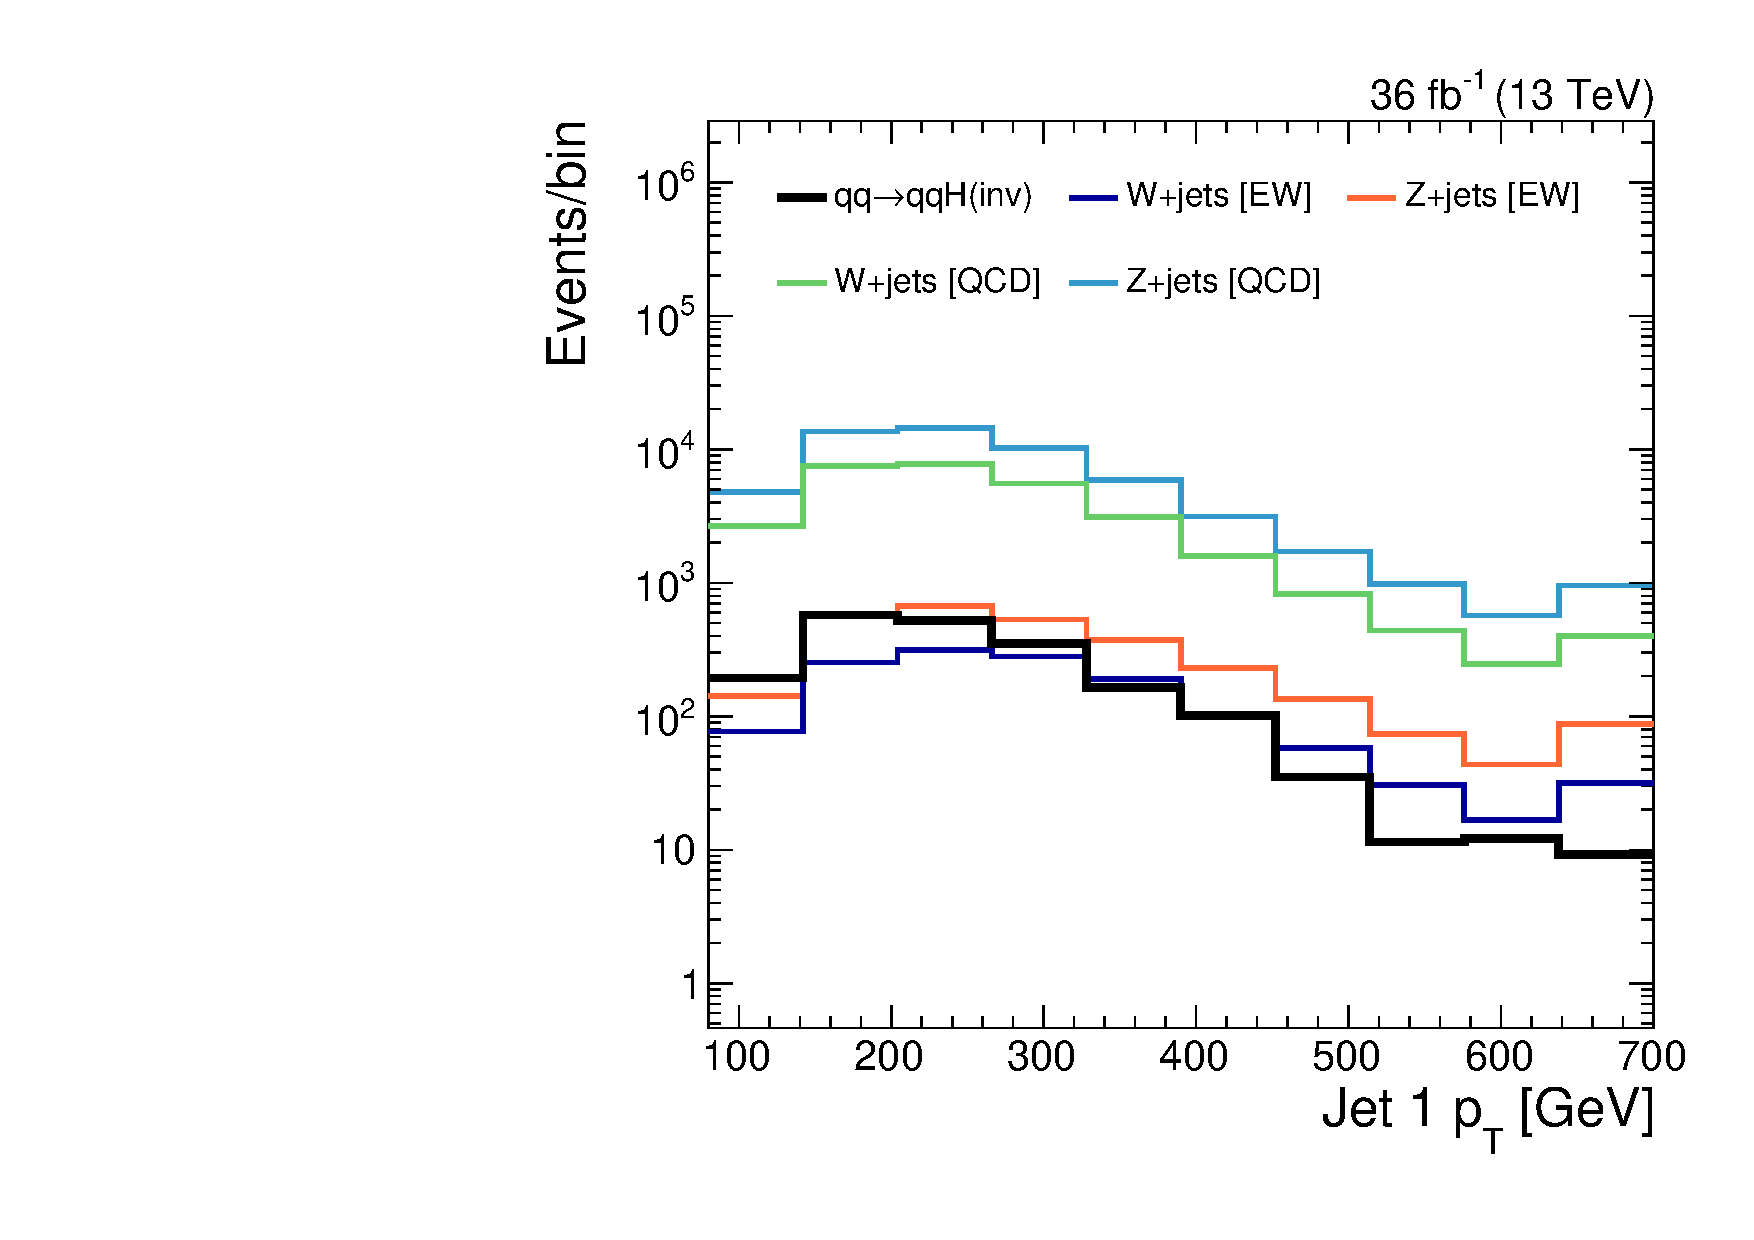
\includegraphics[width=\textwidth]{figures/vbf/shapes/loosesignal_jotPt_0__logy.pdf}
            \caption{Leading jet $\pt$}
        \end{subfigure}
        \begin{subfigure}[t]{0.32\textwidth}
            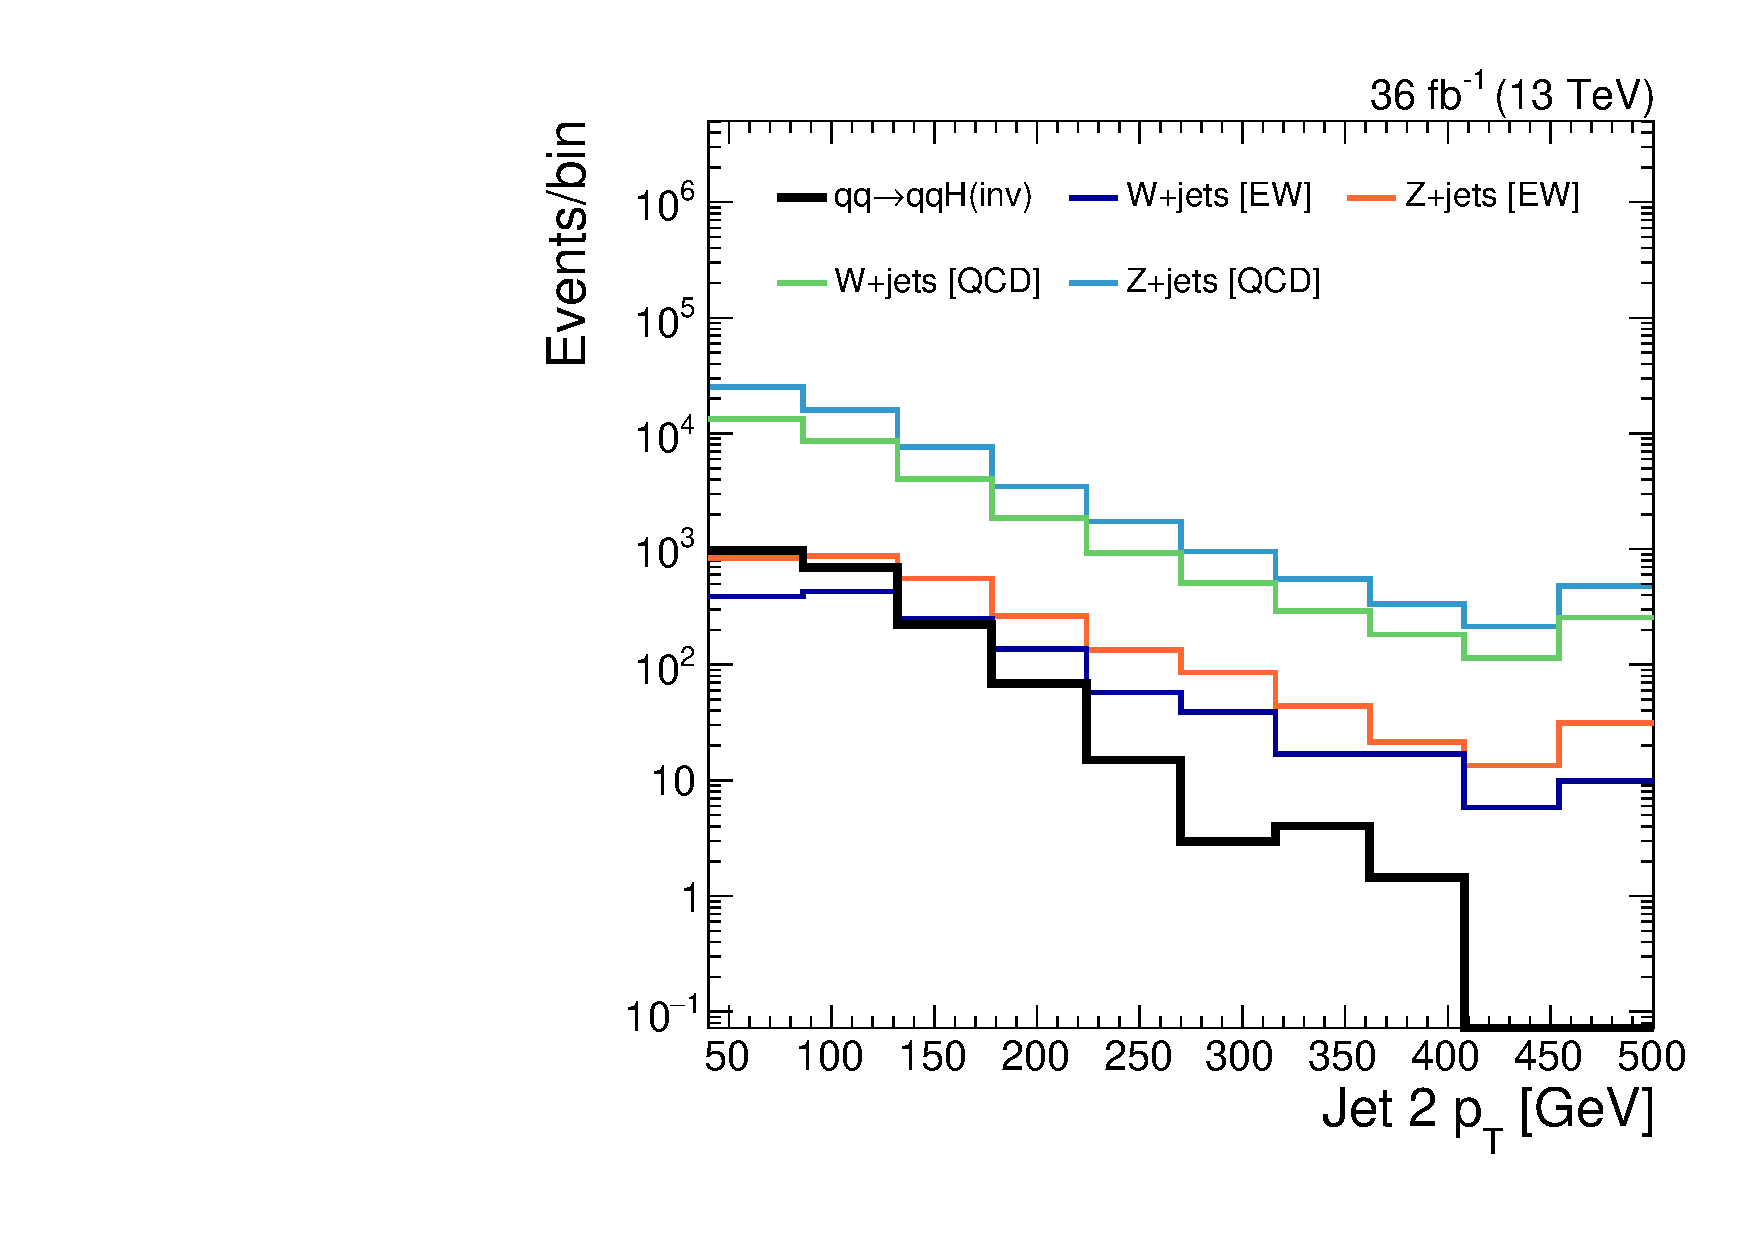
\includegraphics[width=\textwidth]{figures/vbf/shapes/loosesignal_jotPt_1__logy.pdf}
            \caption{Sub-leading jet $\pt$}
        \end{subfigure}
        \begin{subfigure}[t]{0.32\textwidth}
            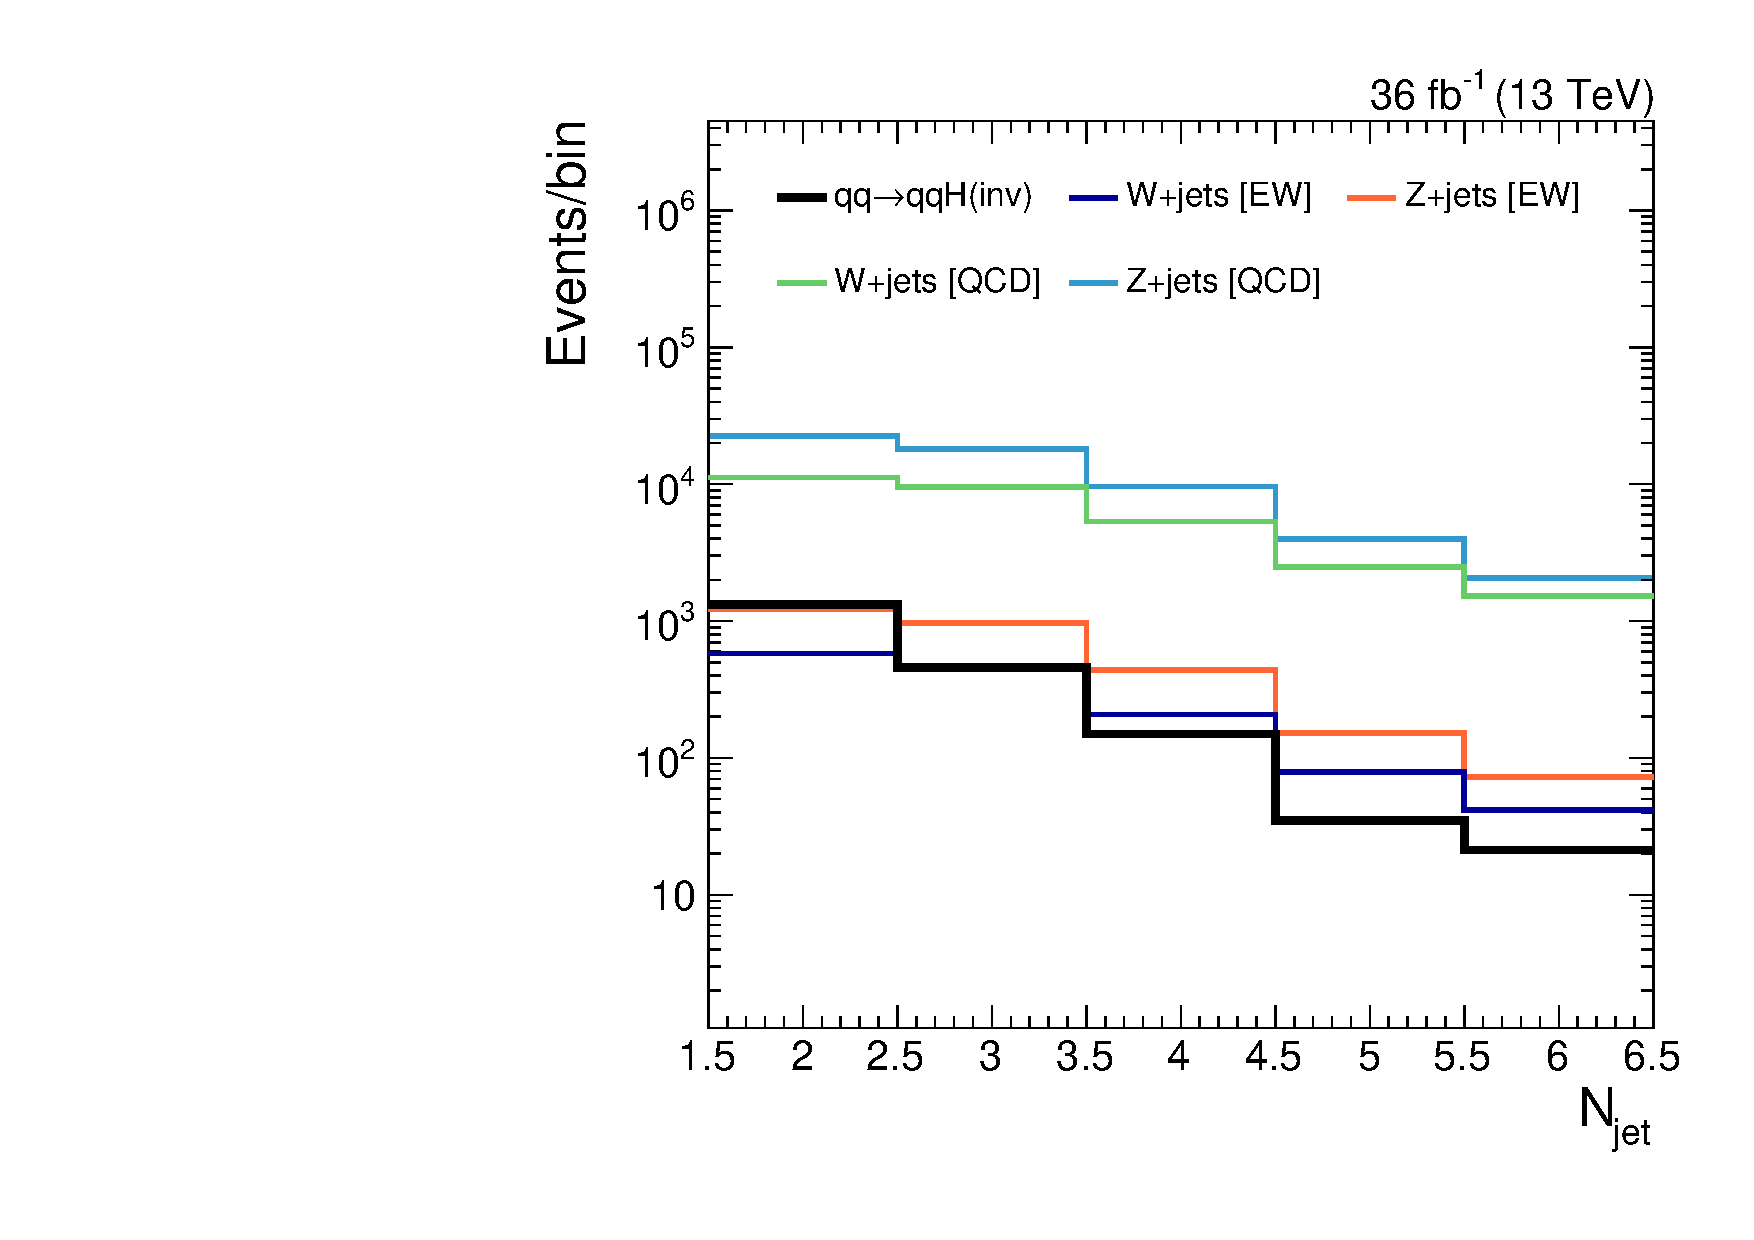
\includegraphics[width=\textwidth]{figures/vbf/shapes/loosesignal_nJot_logy.pdf}
            \caption{$N_\mathrm{jet}$}
        \end{subfigure}
        \begin{subfigure}[t]{0.32\textwidth}
            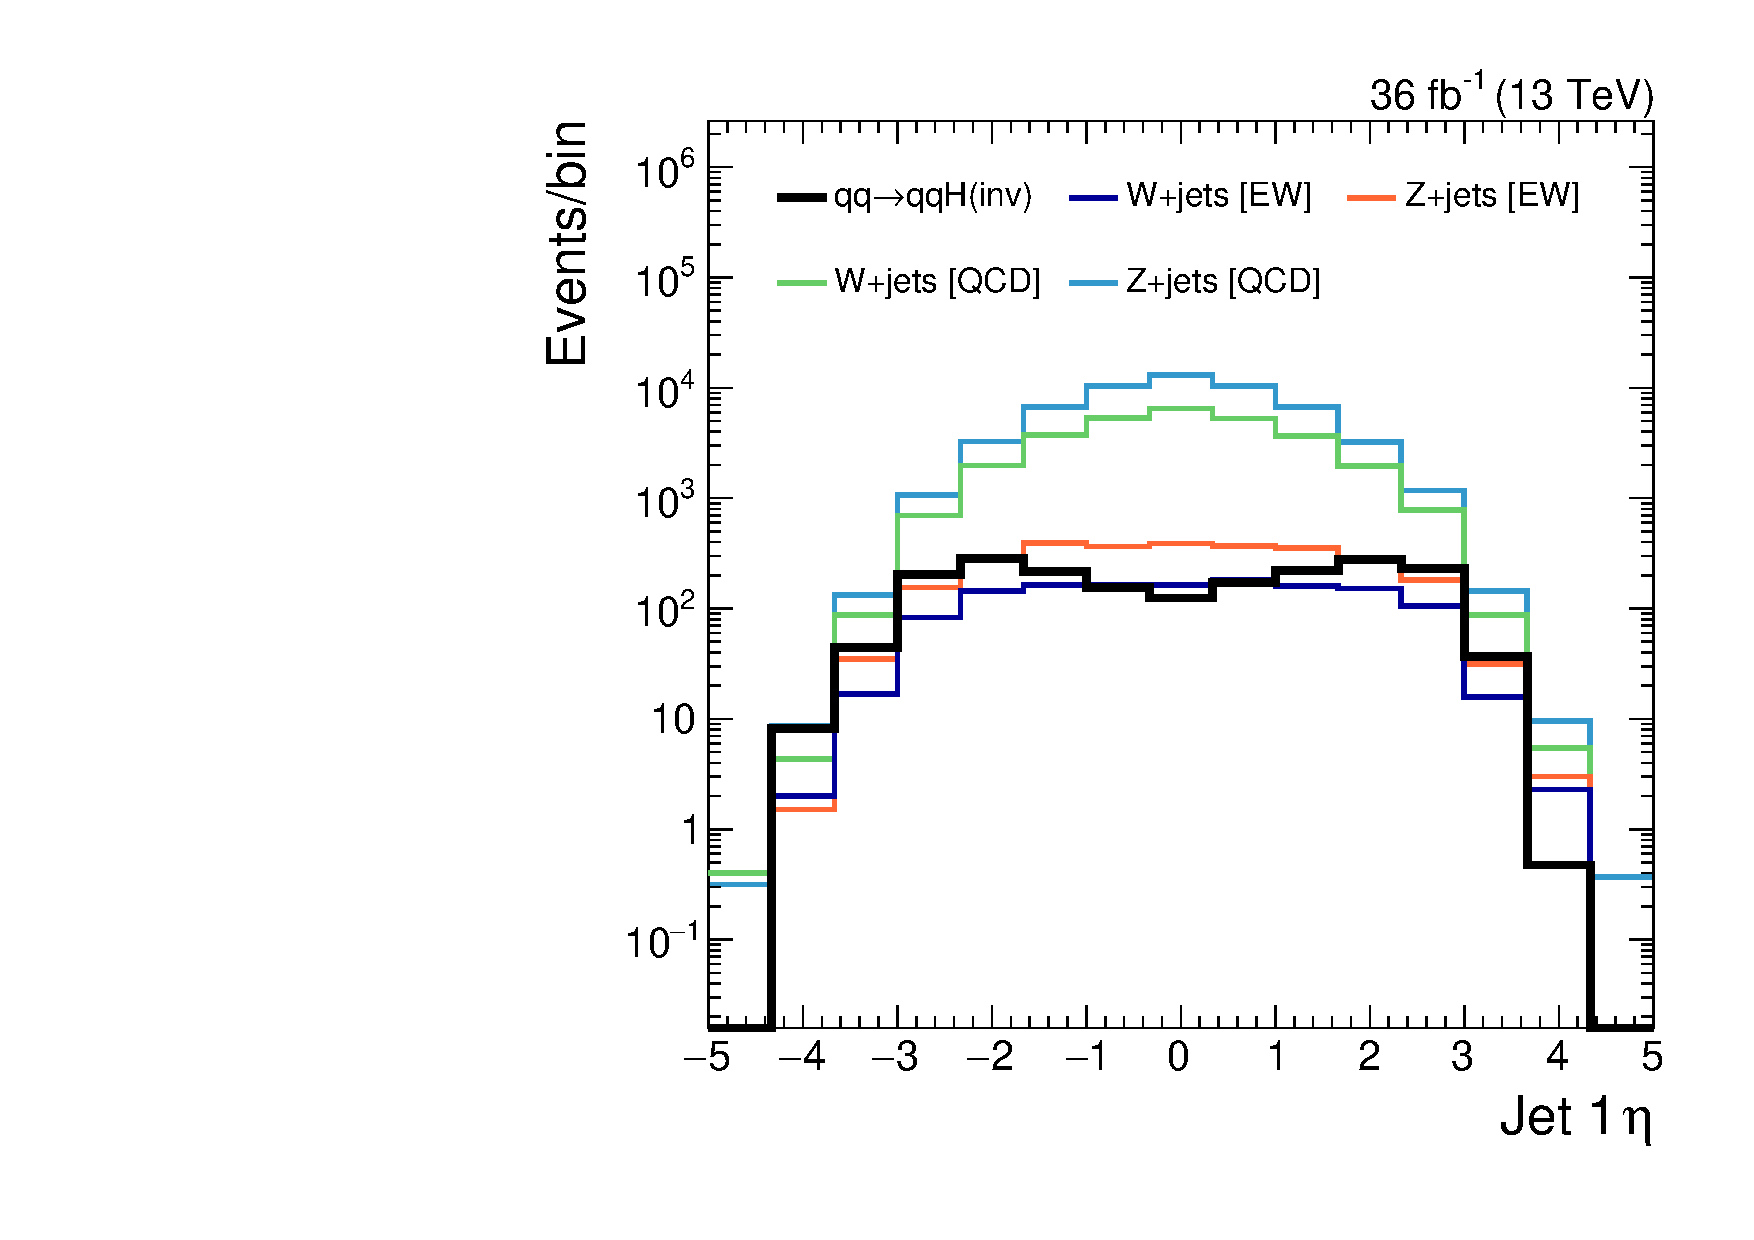
\includegraphics[width=\textwidth]{figures/vbf/shapes/loosesignal_jotEta_0__logy.pdf}
            \caption{Leading jet $\eta$}
        \end{subfigure}
        \begin{subfigure}[t]{0.32\textwidth}
            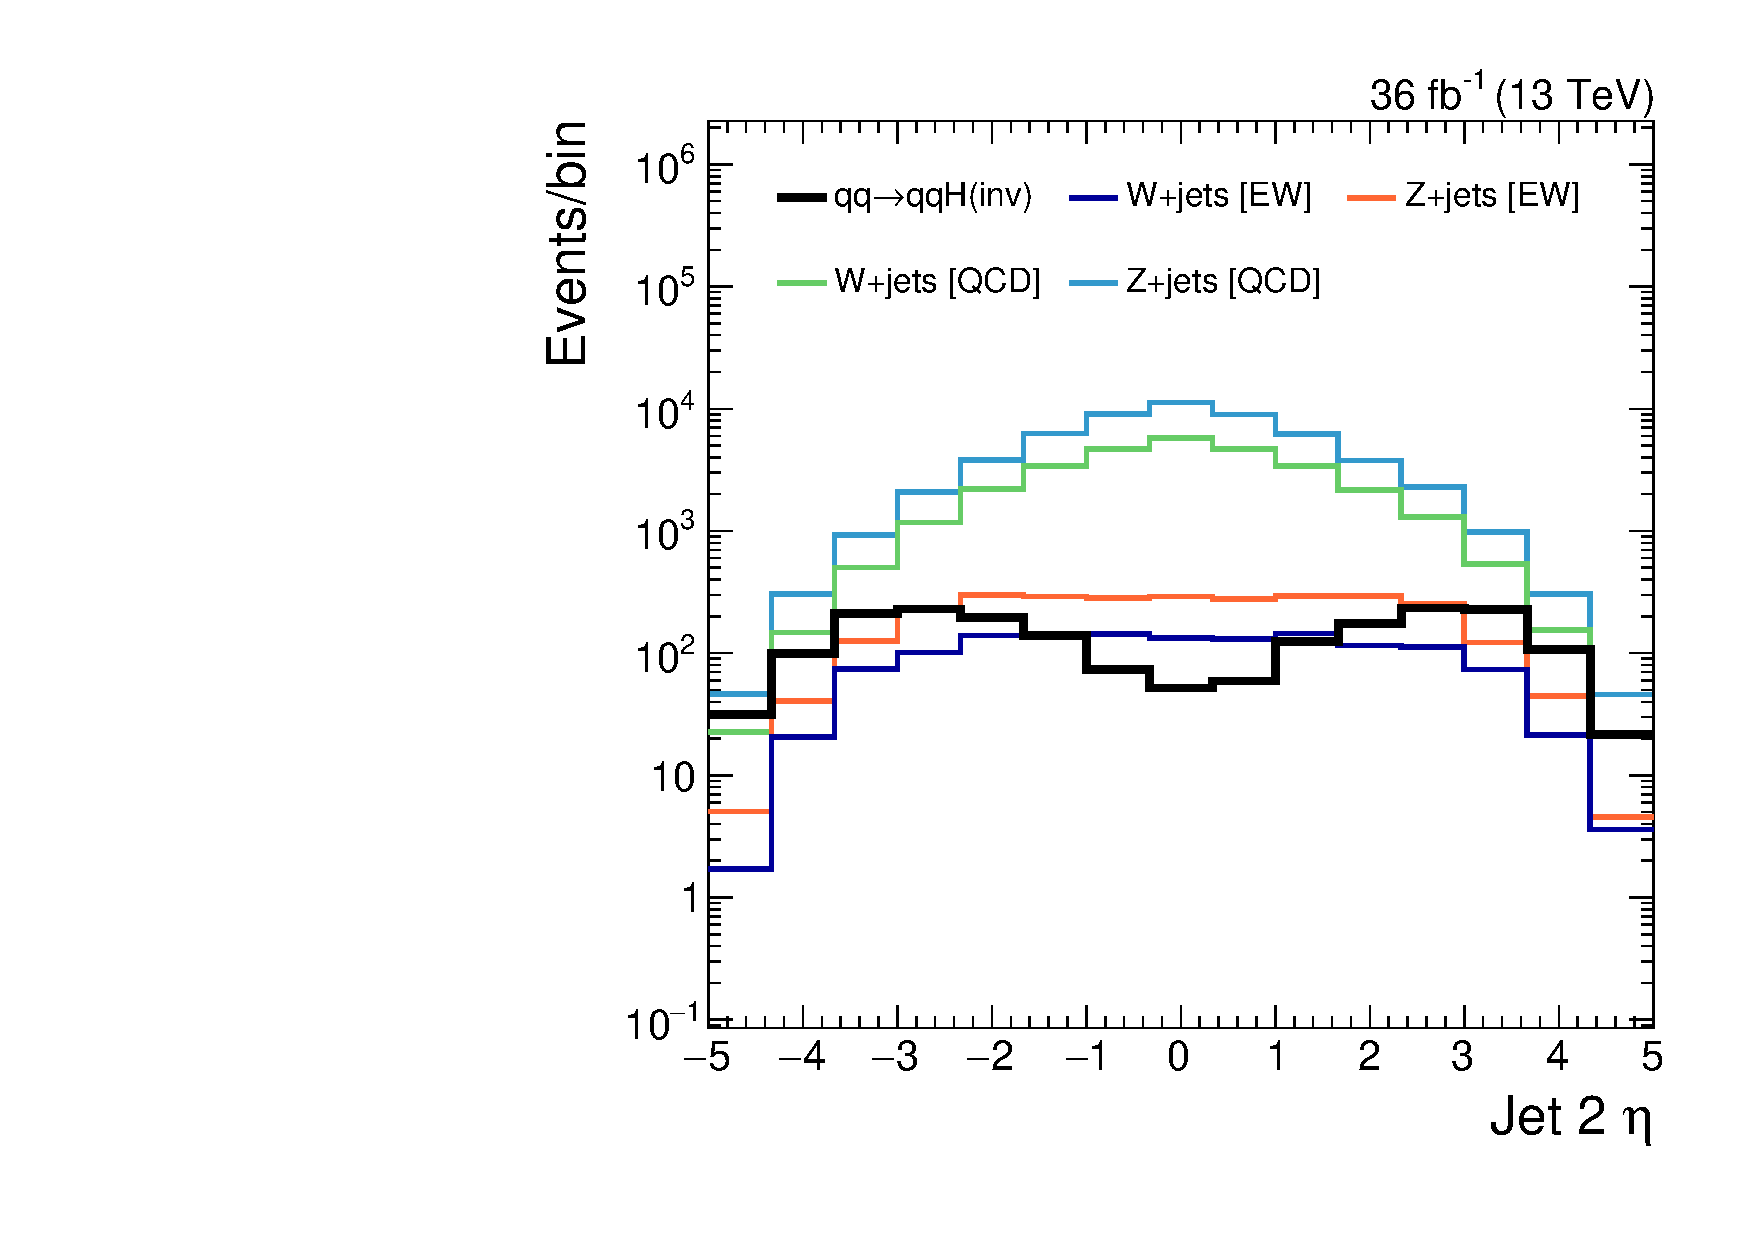
\includegraphics[width=\textwidth]{figures/vbf/shapes/loosesignal_jotEta_1__logy.pdf}
            \caption{Sub-leading jet $\eta$}
        \end{subfigure}
        \begin{subfigure}[t]{0.32\textwidth}
            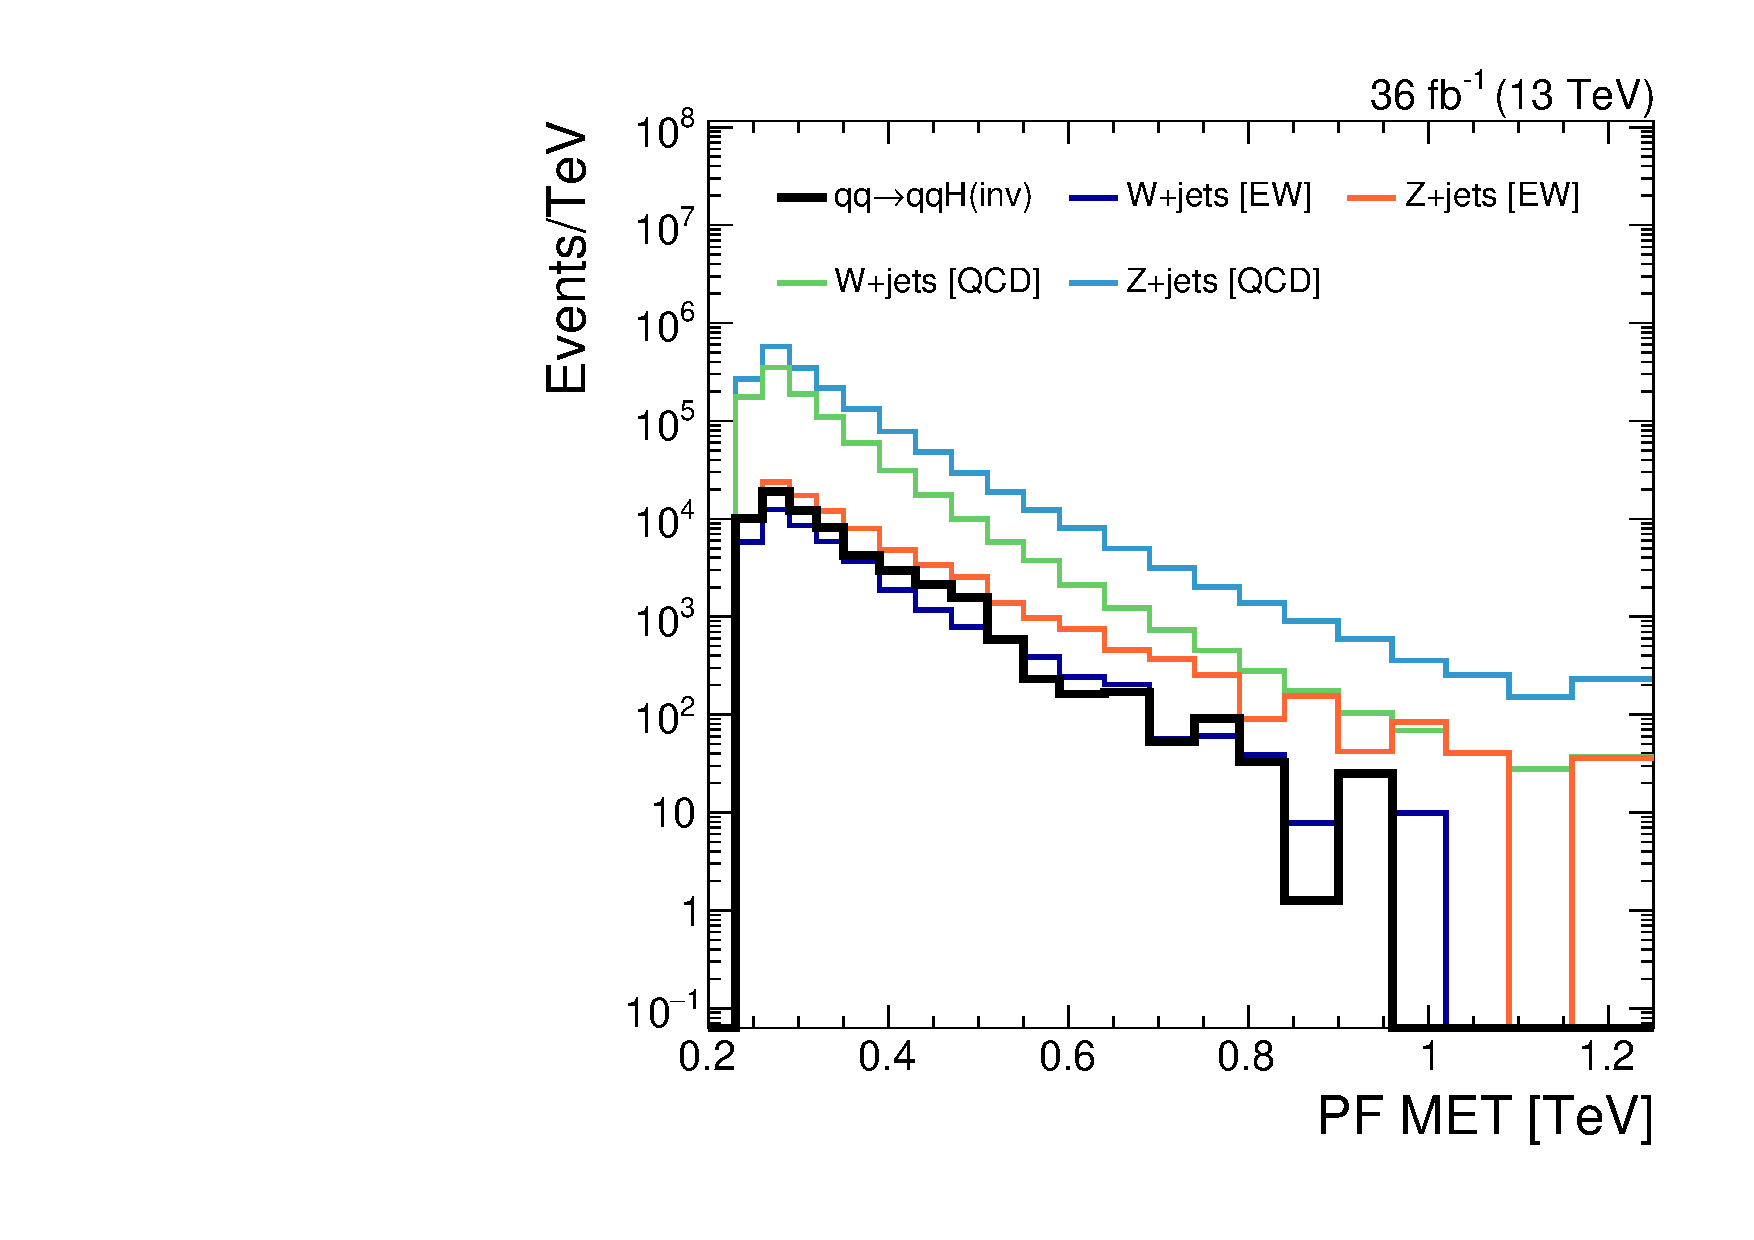
\includegraphics[width=\textwidth]{figures/vbf/shapes/loosesignal_pfmet_logy.pdf}
            \caption{$\ptmiss$}
        \end{subfigure}
        \caption{Event kinematic distributions, as compared between $H$ vs $Z$ vs $W$ production, and VBF vs QCD modes.}
        \label{fig:vbf:jetkins}
    \end{center}
\end{figure}

To fully exploit these kinematic distributions, we look at ``VBF-tag'' observables, which are functions of the two leading jets. 
These are defined as:
\begin{itemize}
    \item[$m_{jj}$:] Invariant mass of the dijet system.
    \item[$\Delta\eta_{jj}$:] Absolute value of the difference in pseudorapidity of the two jets.
    \item[$\Delta\phi_{jj}$:] Absolute value of the difference in azimuthal angle of the two jets.
\end{itemize}
These distributions are shown in Figure~\ref{fig:vbf:dijetkins}.
The first two distributions look different in QCD and VBF processes and are therefore useful to reduce QCD backgrounds.
On the other hand, \dphi~is sensitive to the spin of the boson produced in a VBF process, and therefore can distinguish between Higgs and electroweak boson production.

\begin{figure}[]
    \begin{center}
        \begin{subfigure}[t]{0.32\textwidth}
            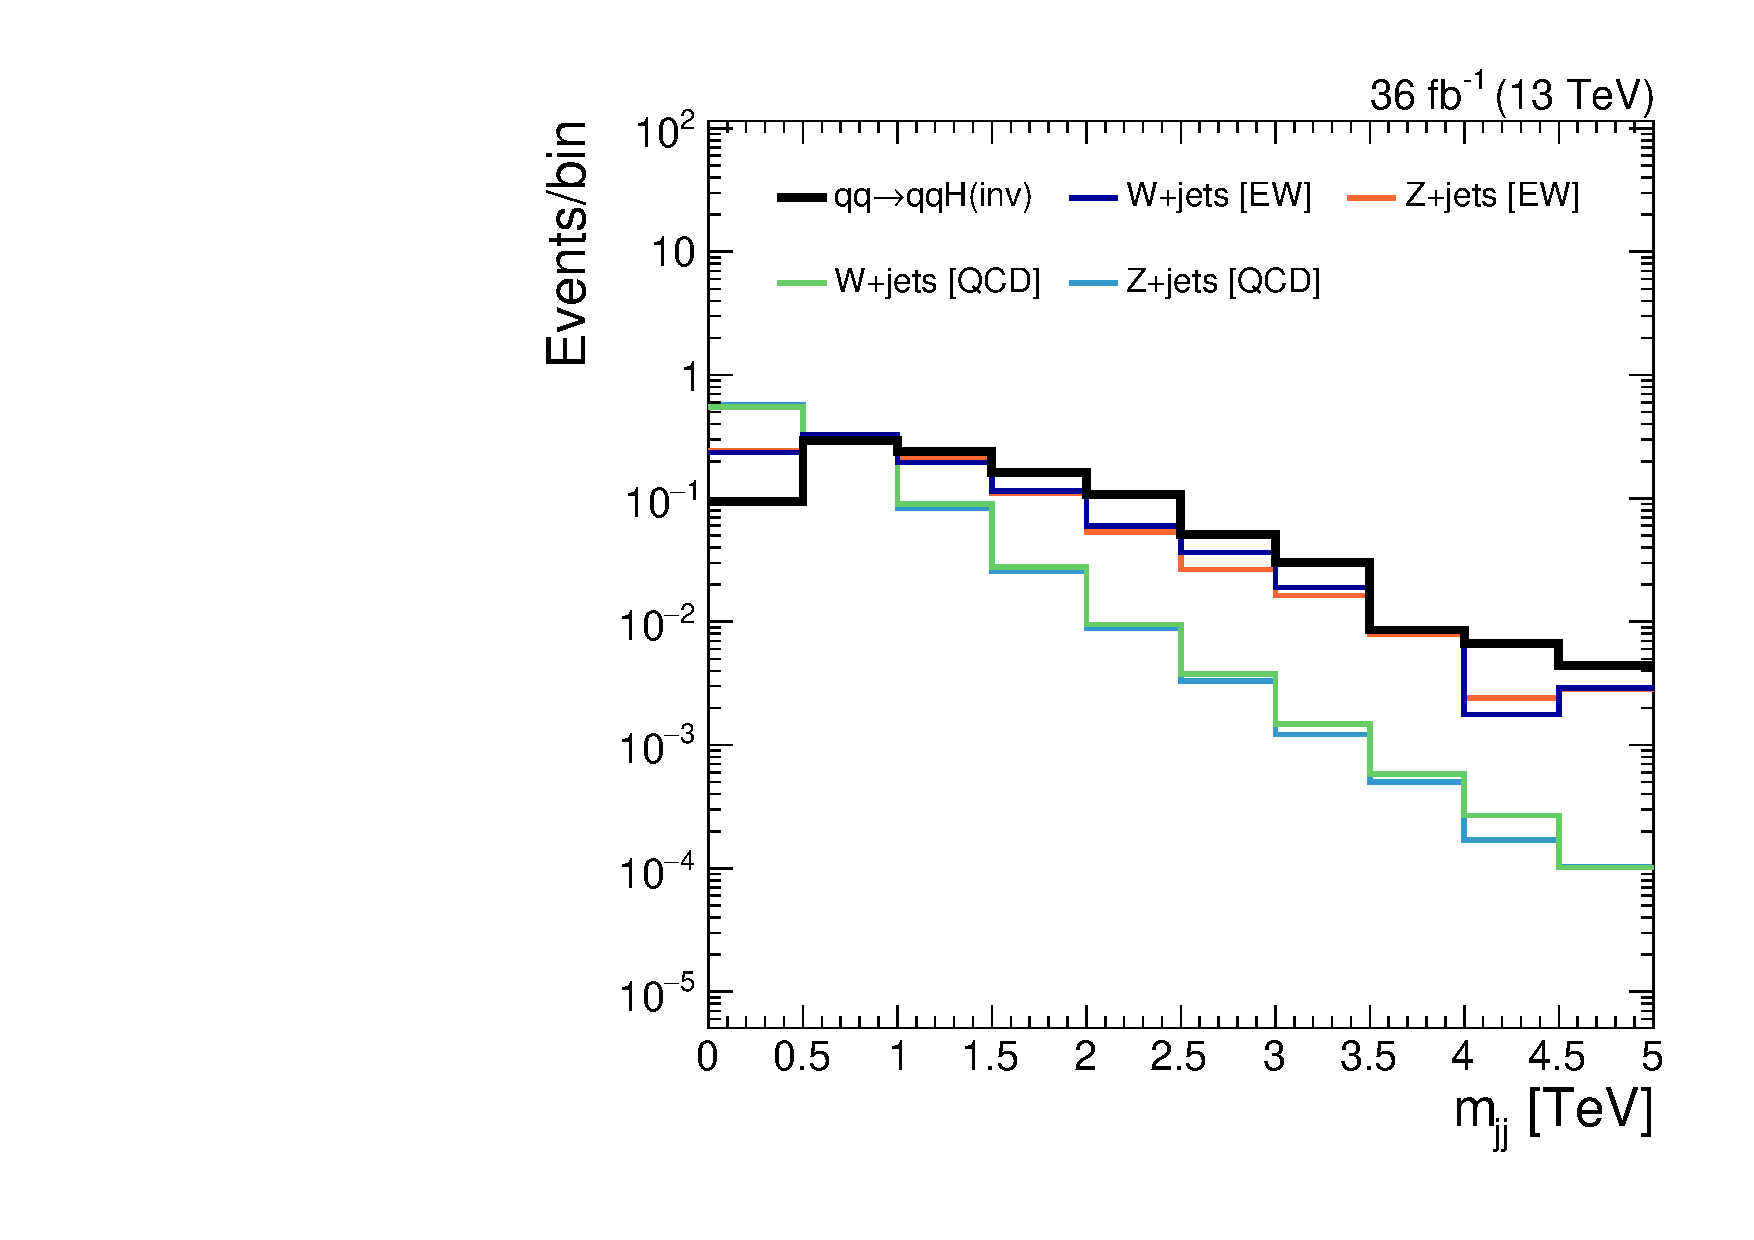
\includegraphics[width=\textwidth]{figures/vbf/shapes/loosesignal_jot12Mass_logy.pdf}
            \caption{\mjj}
        \end{subfigure}
        \begin{subfigure}[t]{0.32\textwidth}
            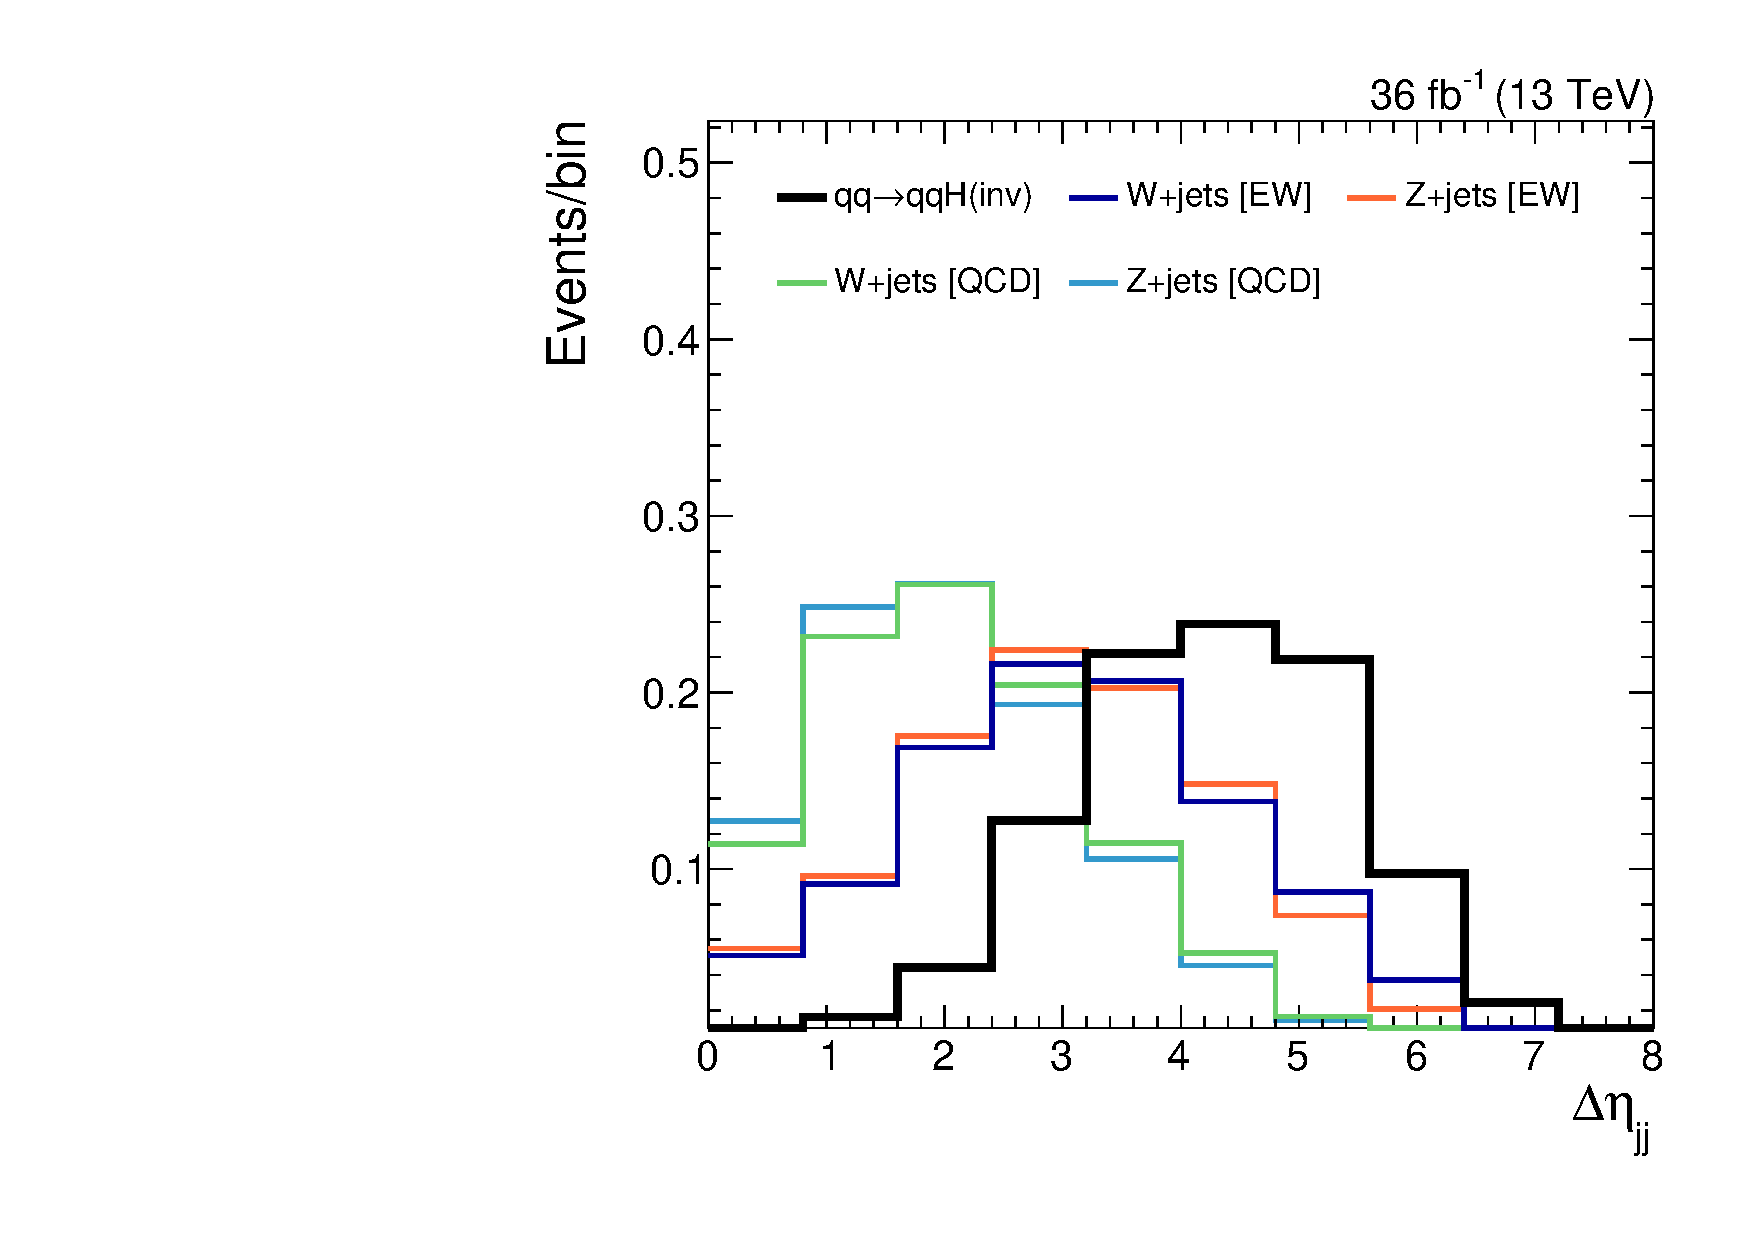
\includegraphics[width=\textwidth]{figures/vbf/shapes/loosesignal_jot12DEta.pdf}
            \caption{\deta}
        \end{subfigure}
        \begin{subfigure}[t]{0.32\textwidth}
            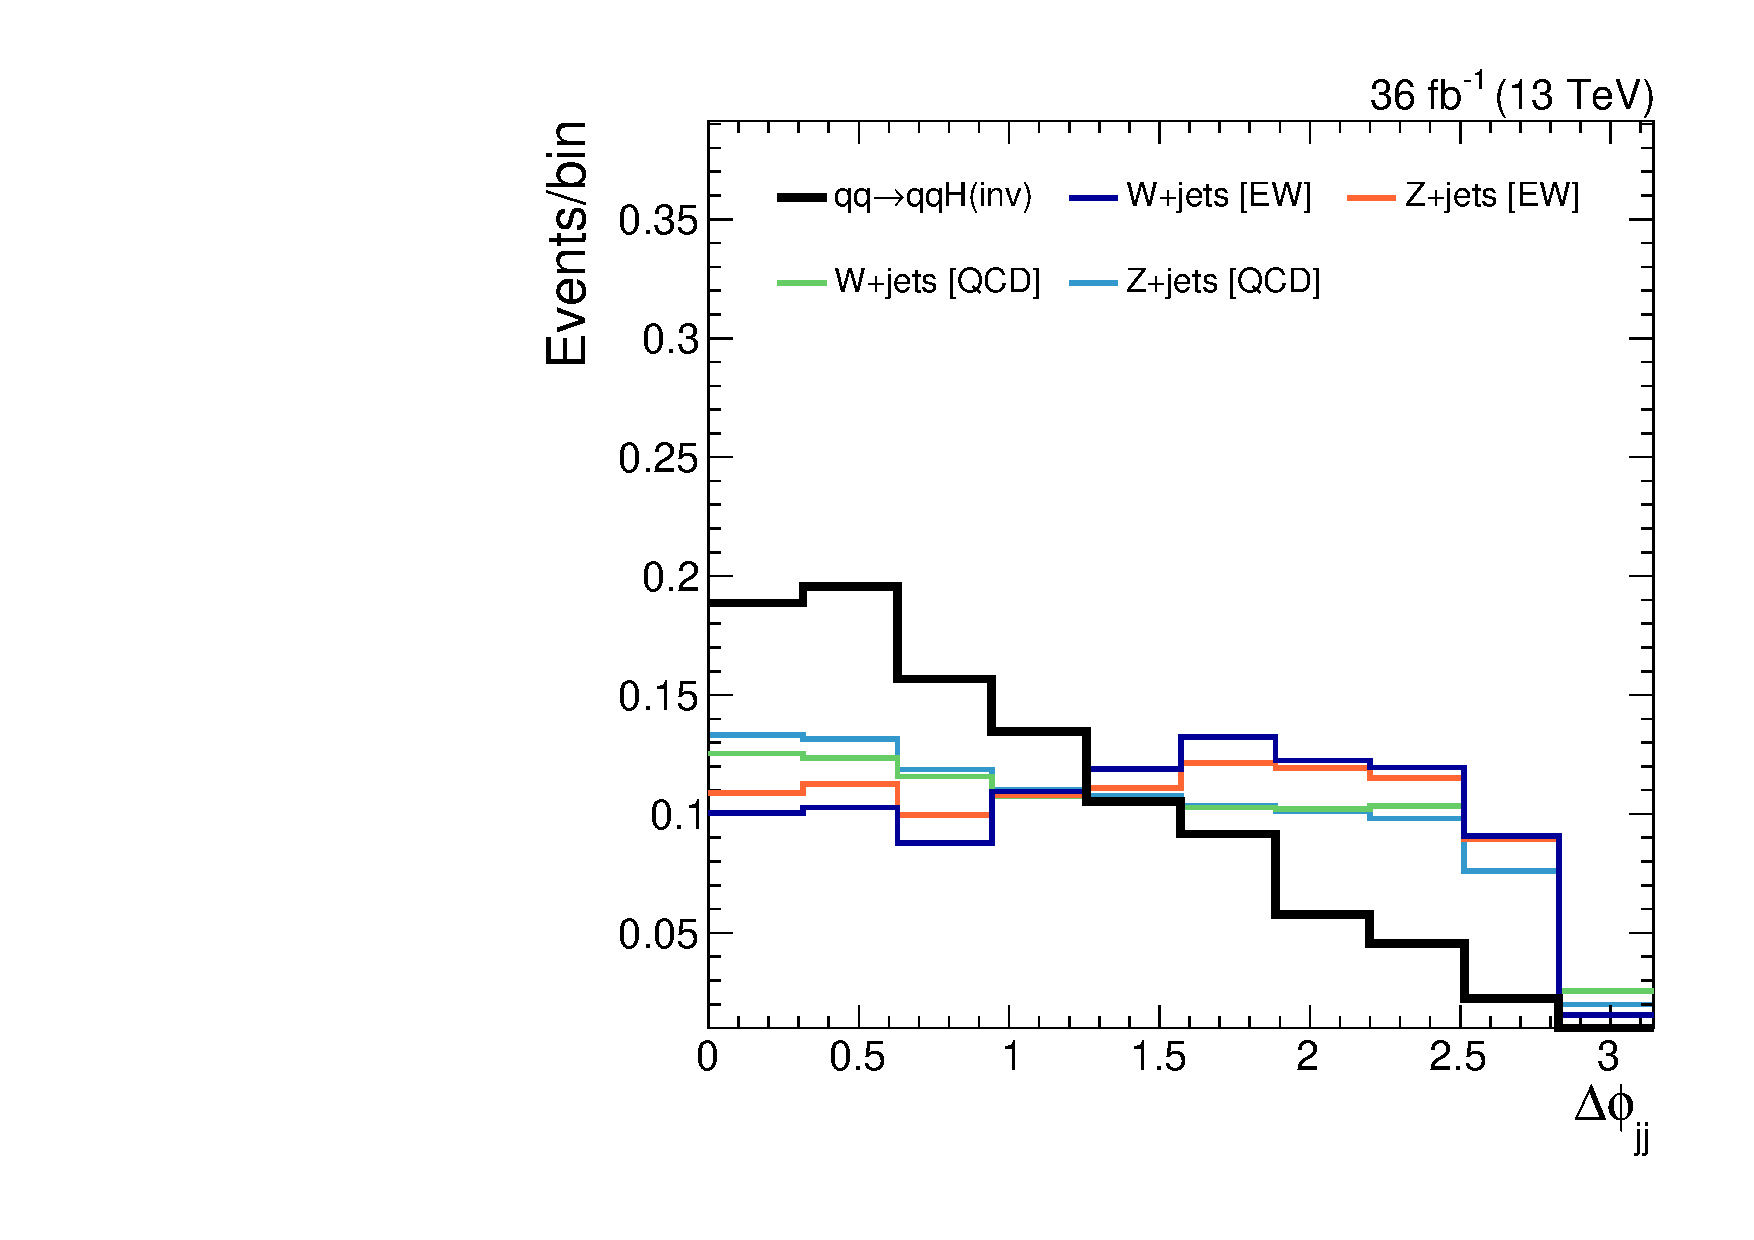
\includegraphics[width=\textwidth]{figures/vbf/shapes/loosesignal_jot12DPhi.pdf}
            \caption{\dphi}
        \end{subfigure}
        \caption{VBF tag observable distributions, as compared between $H$ vs $Z$ vs $W$ production, and VBF vs QCD modes.}
        \label{fig:vbf:dijetkins}
    \end{center}
\end{figure}

\subsection{Sensitivity optimization}

A ``baseline'' selection is defined as:
\begin{itemize}
    \item $\ptmiss>250$ GeV: driven by trigger efficiency, as discussed in Section~\ref{sec:vbf:trig}.
    \item $\pt^\mathrm{jet}>80,40$ GeV: require two VBF jets, lower $\pt$ thresholds set by trigger efficiency
    \item $N_{e,\mu,\tau,\gamma}=0$: veto leptonic decays of $Z$ and $W$, $t\bar{t}$, diboson production, $\gamma$+jet, etc.
    \item $\min\Delta\phi(\mathrm{jet},\ptmiss)>0.4$: remove QCD multijet events.
    \item $|p^\mathrm{miss}_\mathrm{T,calo}-\ptmiss|<\ptmiss/2$: remove miscalibrated events.
\end{itemize}

As the tag variables each show some level of separation between signal and backgrounds, we can choose to either fit the distributions or use them to select events. 
To find the optimal choice, we fit each of the distributions in turn, and scan the other two observables.
The details of this fit and the background estimation are described in Section~\ref{sec:vbf:bkg}.
The metric is chosen to be the expected 95\% CLs upper limit on $\mathcal{B}(\hinv)$.
Figure~\ref{fig:vbf:opt} shows the result of this optimization.
The dijet mass is found to be the best distribution to fit, while requiring $\Delta\eta_{jj}>1$ and $\Delta\phi_{jj}<1.5$.

\begin{figure}[]
    \begin{center}
        \begin{subfigure}[t]{0.32\textwidth}
            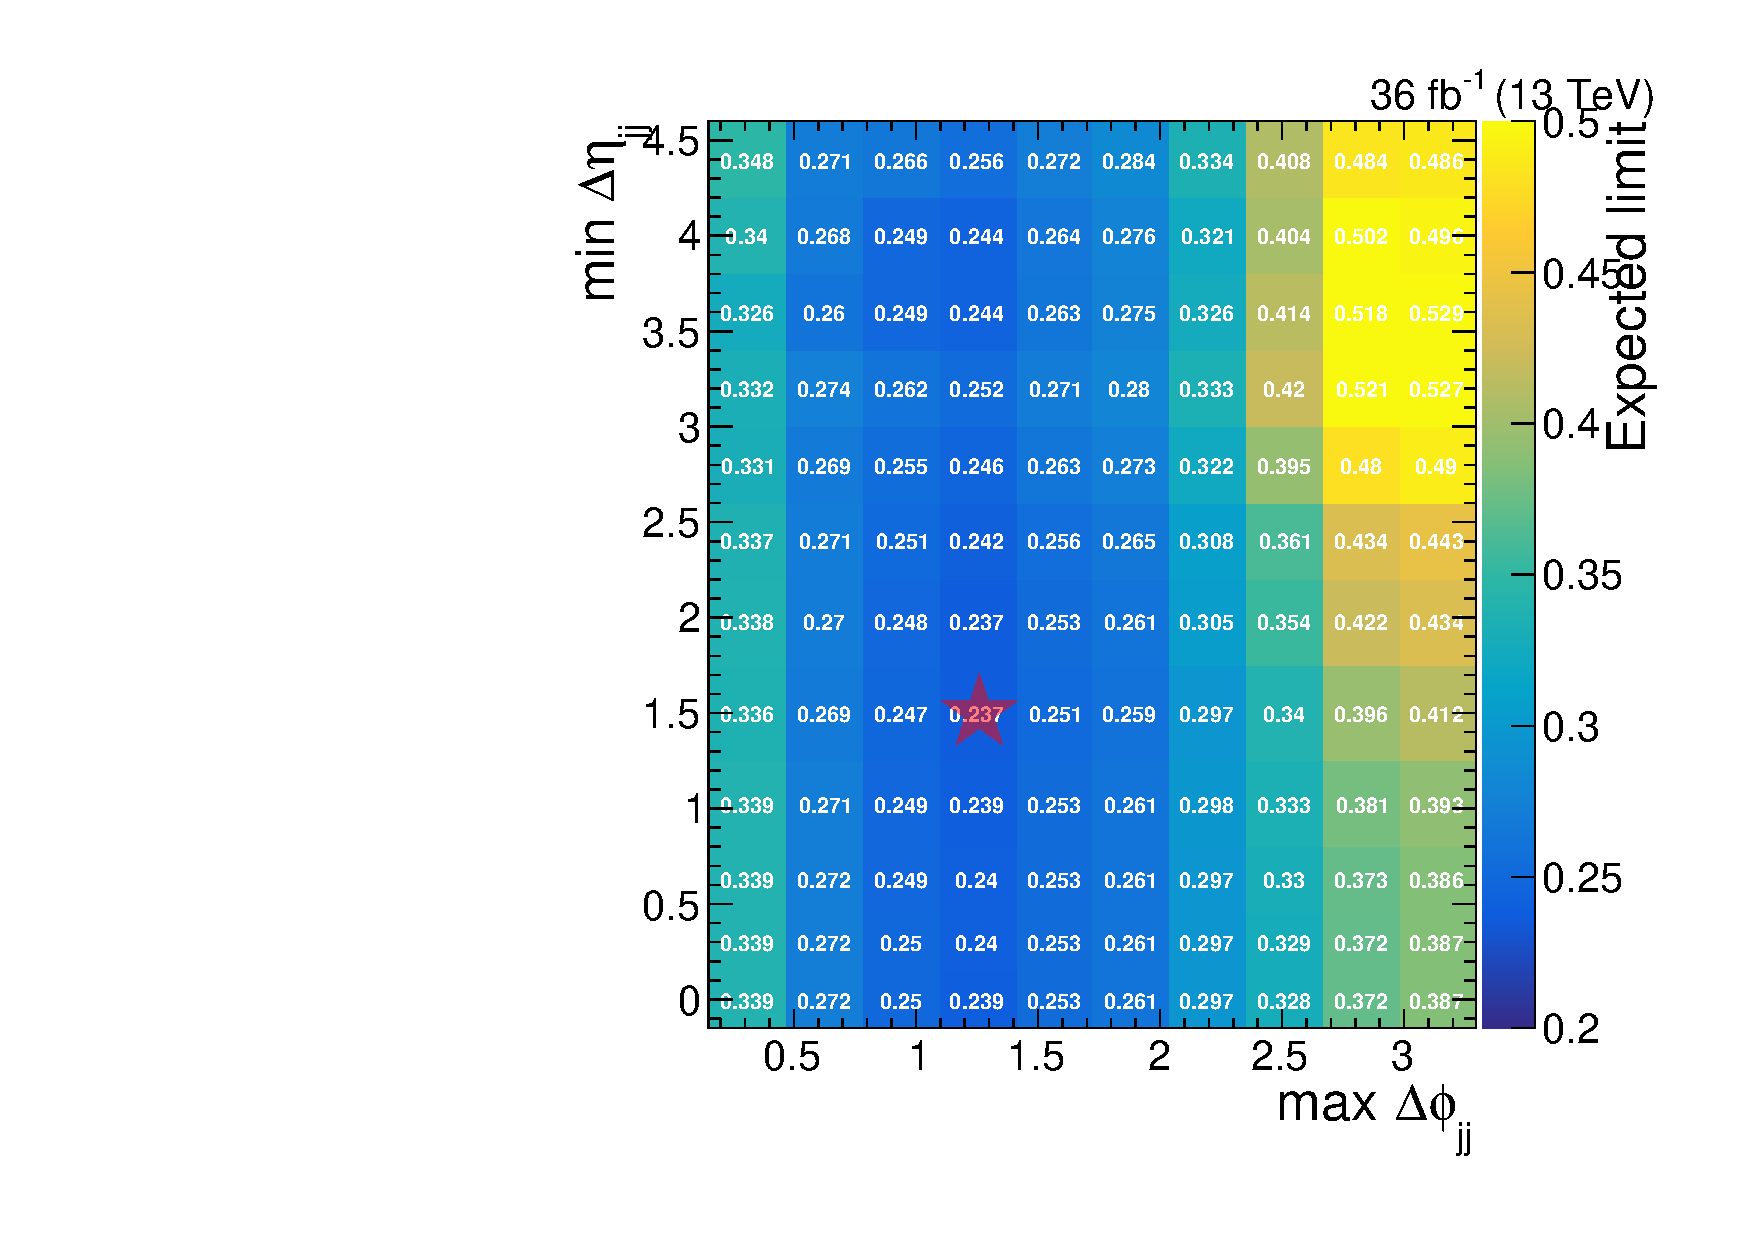
\includegraphics[width=\textwidth]{figures/vbf/opt/optimized_scan_deta_fabsdphi.pdf}
            \caption{Fit \mjj}
        \end{subfigure}
        \begin{subfigure}[t]{0.32\textwidth}
            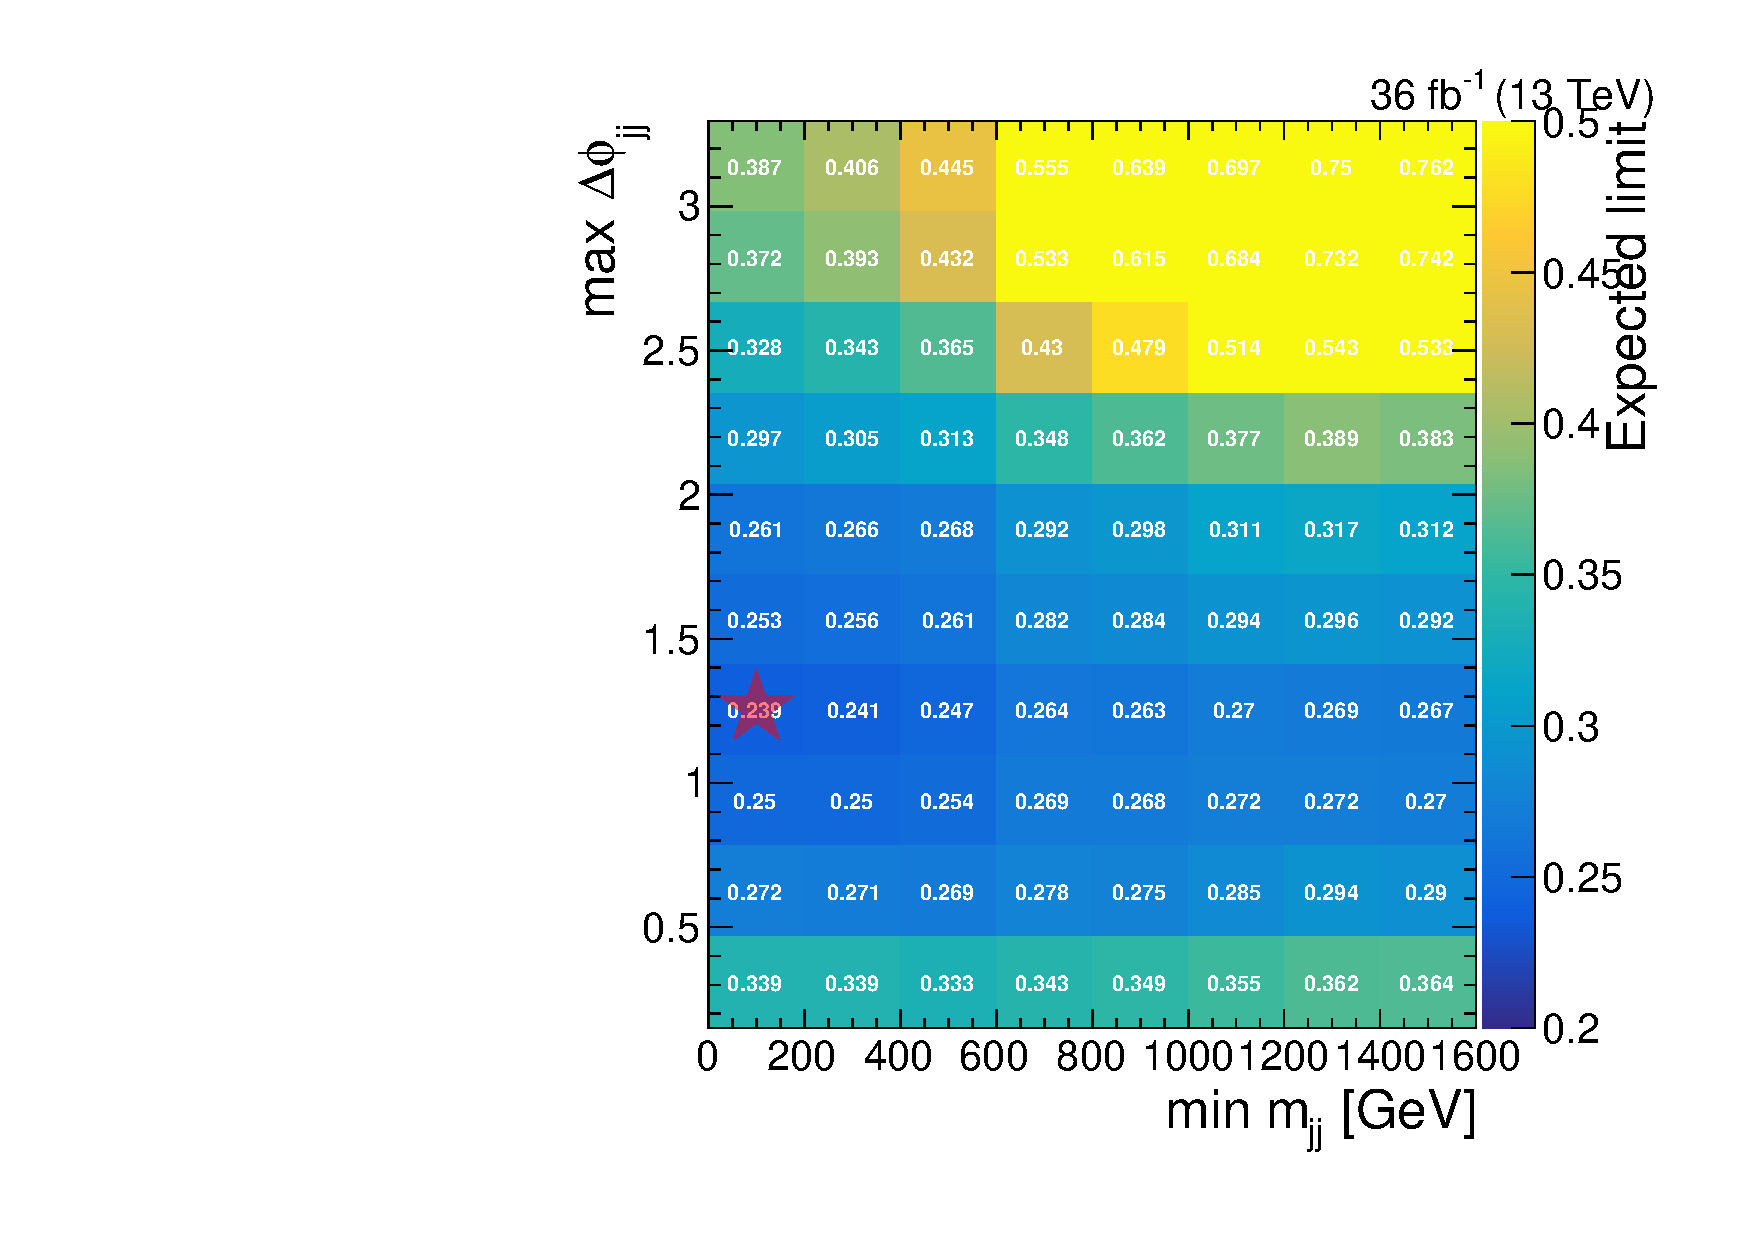
\includegraphics[width=\textwidth]{figures/vbf/opt/optimized_scan_fabsdphi_mjj.pdf}
            \caption{Fit \deta}
        \end{subfigure}
        \begin{subfigure}[t]{0.32\textwidth}
            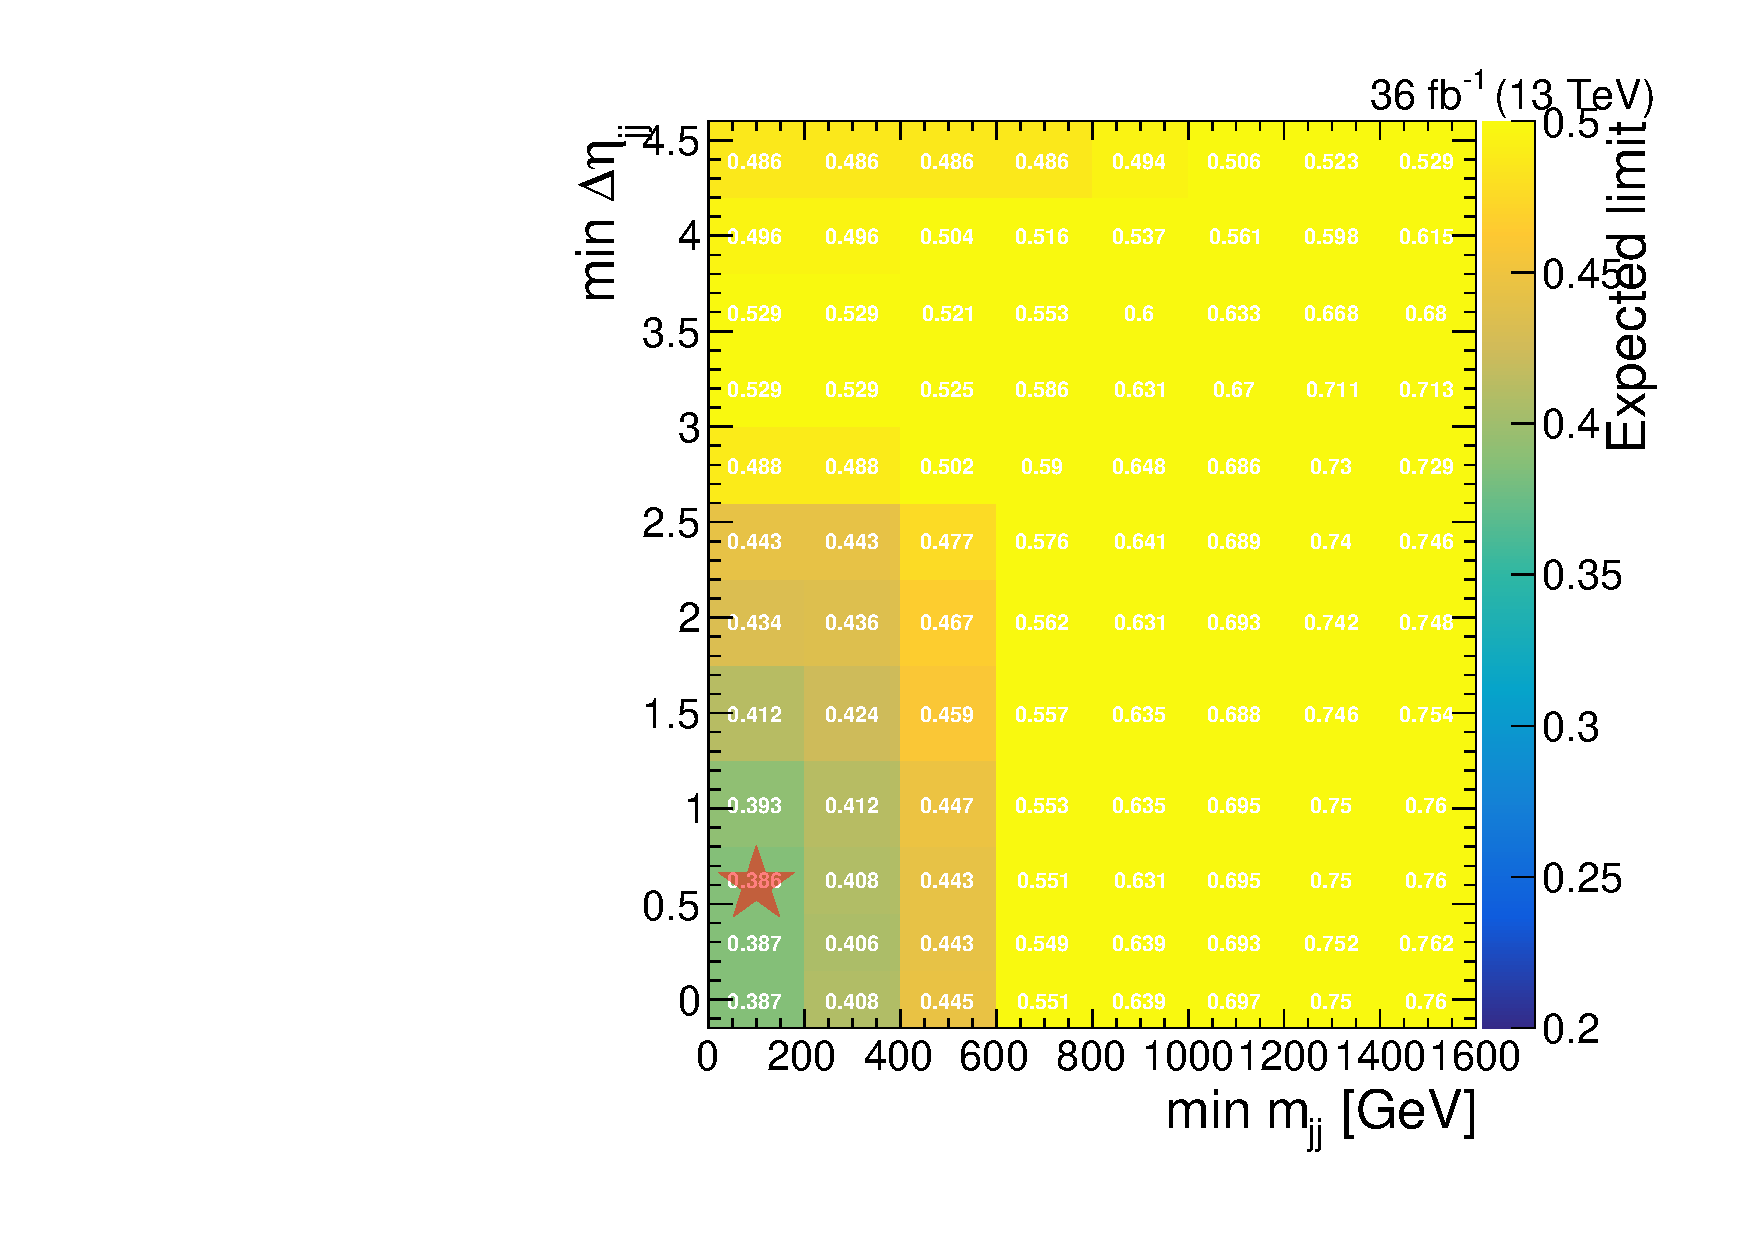
\includegraphics[width=\textwidth]{figures/vbf/opt/optimized_scan_deta_mjj.pdf}
            \caption{Fit \dphi}
        \end{subfigure}
        \caption{Optimization of the dijet kinematic selection, in three different fitting distribution scenarios.}
        \label{fig:vbf:opt}
    \end{center}
\end{figure}

\section{Background estimation}
\label{sec:vbf:bkg}

To estimate the combined $m_{jj}$ spectra of the EW and QCD $V$+jet backgrounds, we employ a similar visible-to-invisible strategy as described in Section~\ref{sec:mt:bkg}.
In this case, the transfer factors $\T{}{}$ are a function of $m_{jj}$.
Control regions are defined using dilepton (single-lepton) selections to estimate the $Z$ ($W$) contributions.
Again, $\ptmiss$ is replaced by $U$ (Equation~\ref{eq:u}) to mimic the signal region selection. 
Because there are \emph{two} components to estimate in each CR (QCD and EW), we slightly modify the likelihood.
Adding only the $\mu\mu$ CR to constrain the $Z$+jet component for now:
\begin{align}
    \mathcal{L}(\bm{d} \,|\, \mu,\muz,\bm{\theta}) = & \prod_{i\in\mathrm{bins}} \left[
    \pois\left(d^{\mathrm{SR}}_{i} ~\Big|~ \mu S^{\mathrm{SR}}_{i}(\bm\theta)  + \muzi + \frac{\muzi}{\Ti{\mathrm{QE}}{Z}(\bm\theta)} + B^{\mathrm{SR}}_{i}(\bm\theta)\right) \right. \nonumber \\
    & \left. \phantom{\prod_{i\in\mathrm{bins}}\Big[} \times \pois\left(d^{\mu\mu}_i~\Big|~ \frac{\muzi}{\Ti{\mu\mu}{Z}(\bm\theta)} + \frac{\muzi}{\Ti{\mu\mu}{Z}(\bm\theta) \Ti{\mathrm{QE}}{Z}(\bm\theta)} + B^{\mu\mu}_i(\bm\theta) \right)\right]  \nonumber \\ 
    & \times  \prod_{j=0}^{n_\theta} p_j(\theta_j)
\end{align}
While the notation largely follows that used in Equation~\ref{eq:mt:lhood}, one additional term has been introduced.
This is a ``transfer factor'' linking the QCD and EW components in the signal region, so that the only free parameter is $\muz$:
\begin{equation}
    \Ti{\mathrm{QE}}{Z} = \frac{N^\mathrm{SR}_i(\mathrm{QCD\,}Z\rightarrow\nu\nu)}{N^\mathrm{SR}_i(\mathrm{EW\,}Z\rightarrow\nu\nu)} 
\end{equation}
where as always, the yields $N$ are predicted using MC. 
Kinematic distributions from the two dilepton CRs are shown in Figure~\ref{fig:vbf:zcr}.

\begin{figure}[]
    \begin{center}
        \begin{subfigure}[t]{0.24\textwidth}
            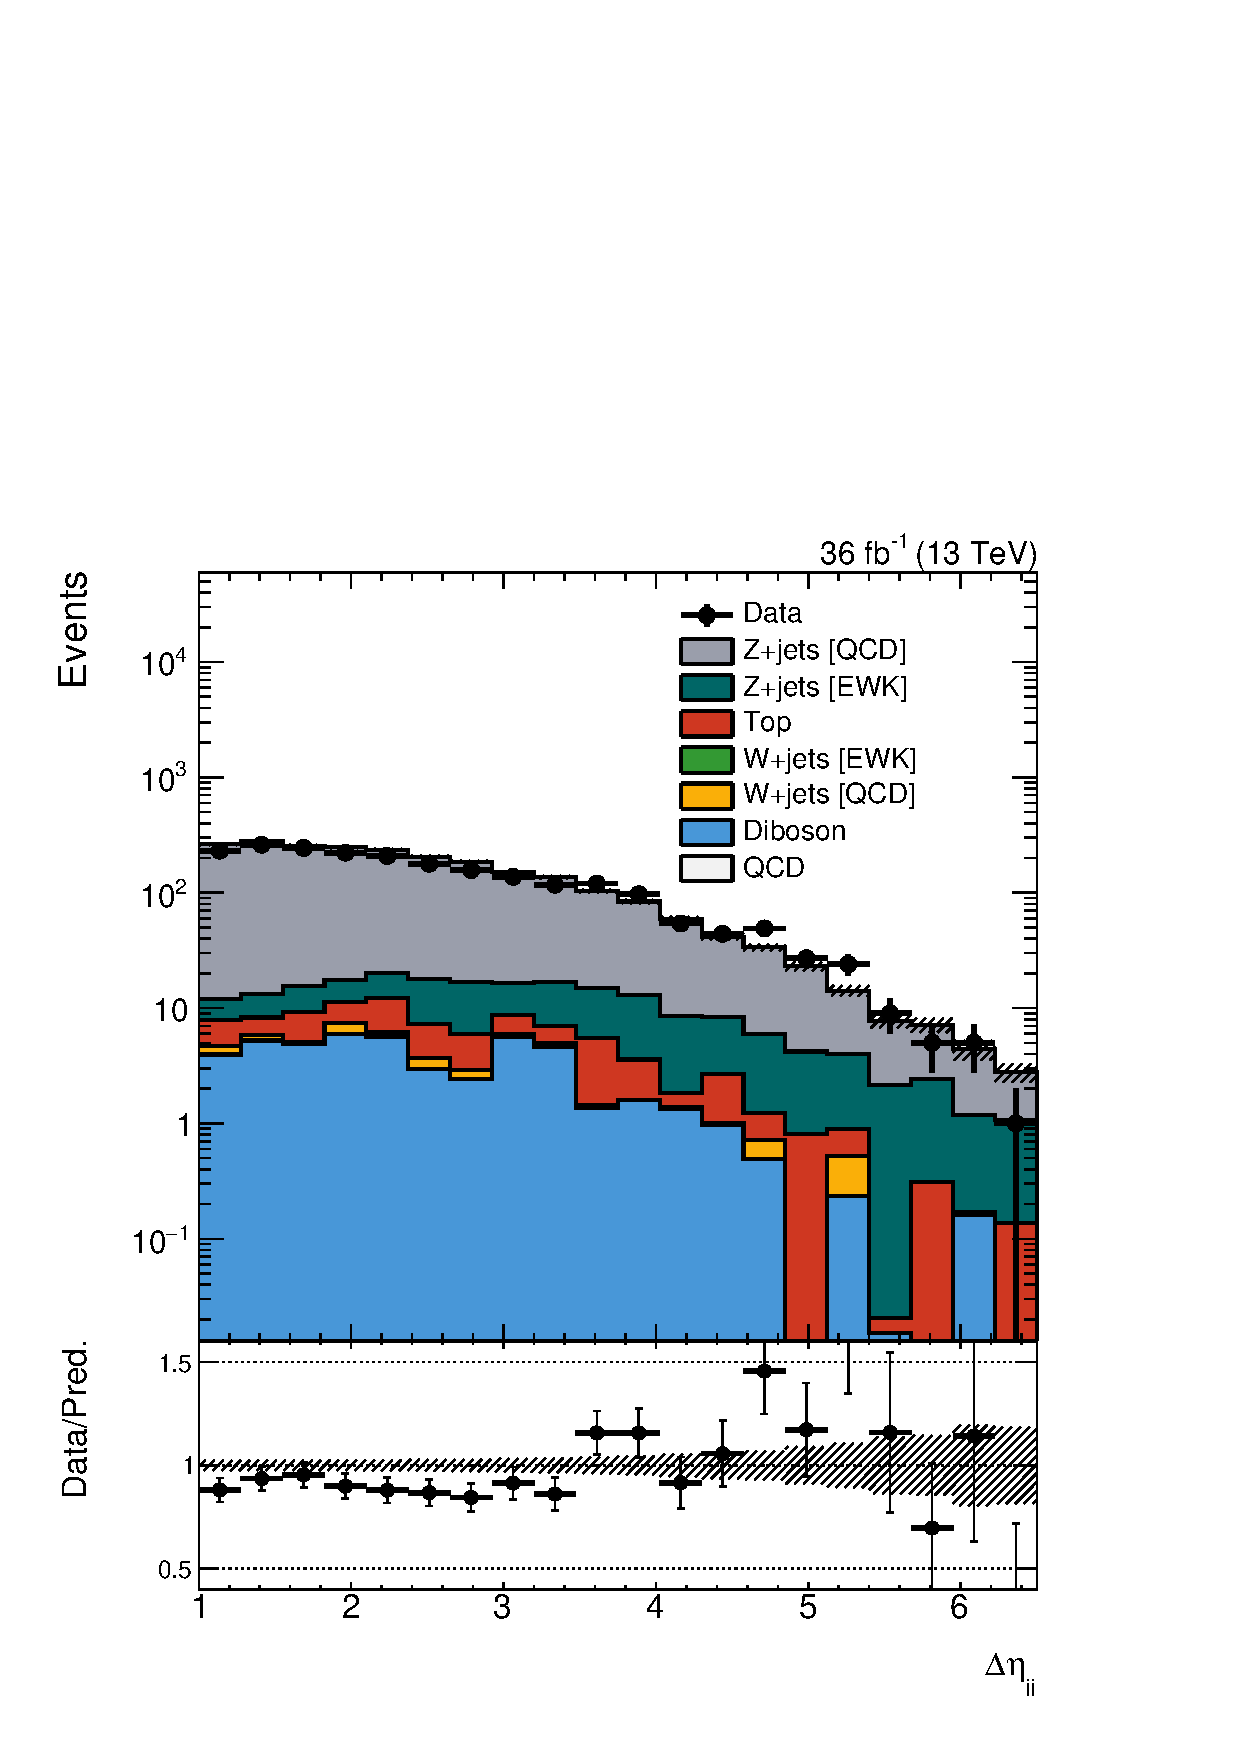
\includegraphics[width=\textwidth]{figures/vbf/prefit/dielectron_jot12DEta_logy.pdf}
        \end{subfigure}
        \begin{subfigure}[t]{0.24\textwidth}
            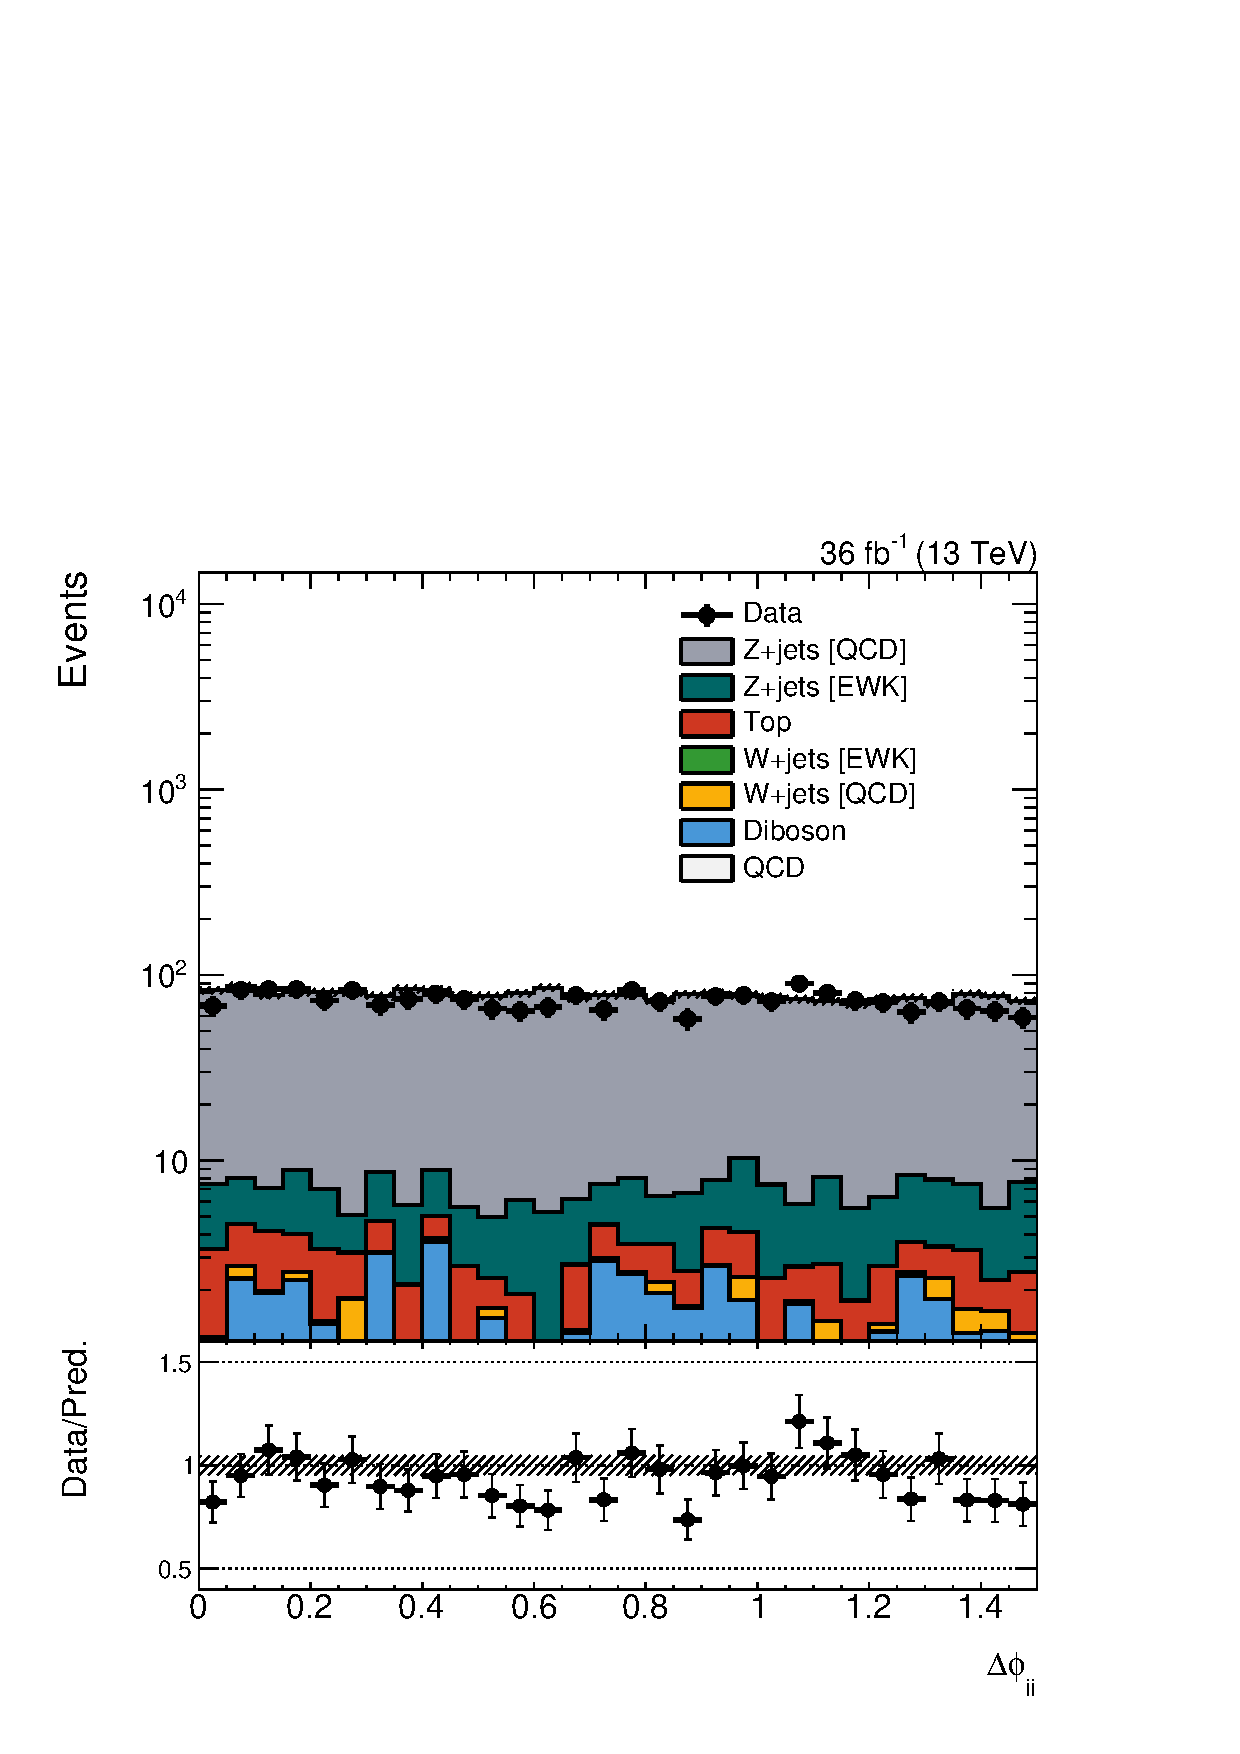
\includegraphics[width=\textwidth]{figures/vbf/prefit/dielectron_jot12DPhi_logy.pdf}
        \end{subfigure}
        \begin{subfigure}[t]{0.24\textwidth}
            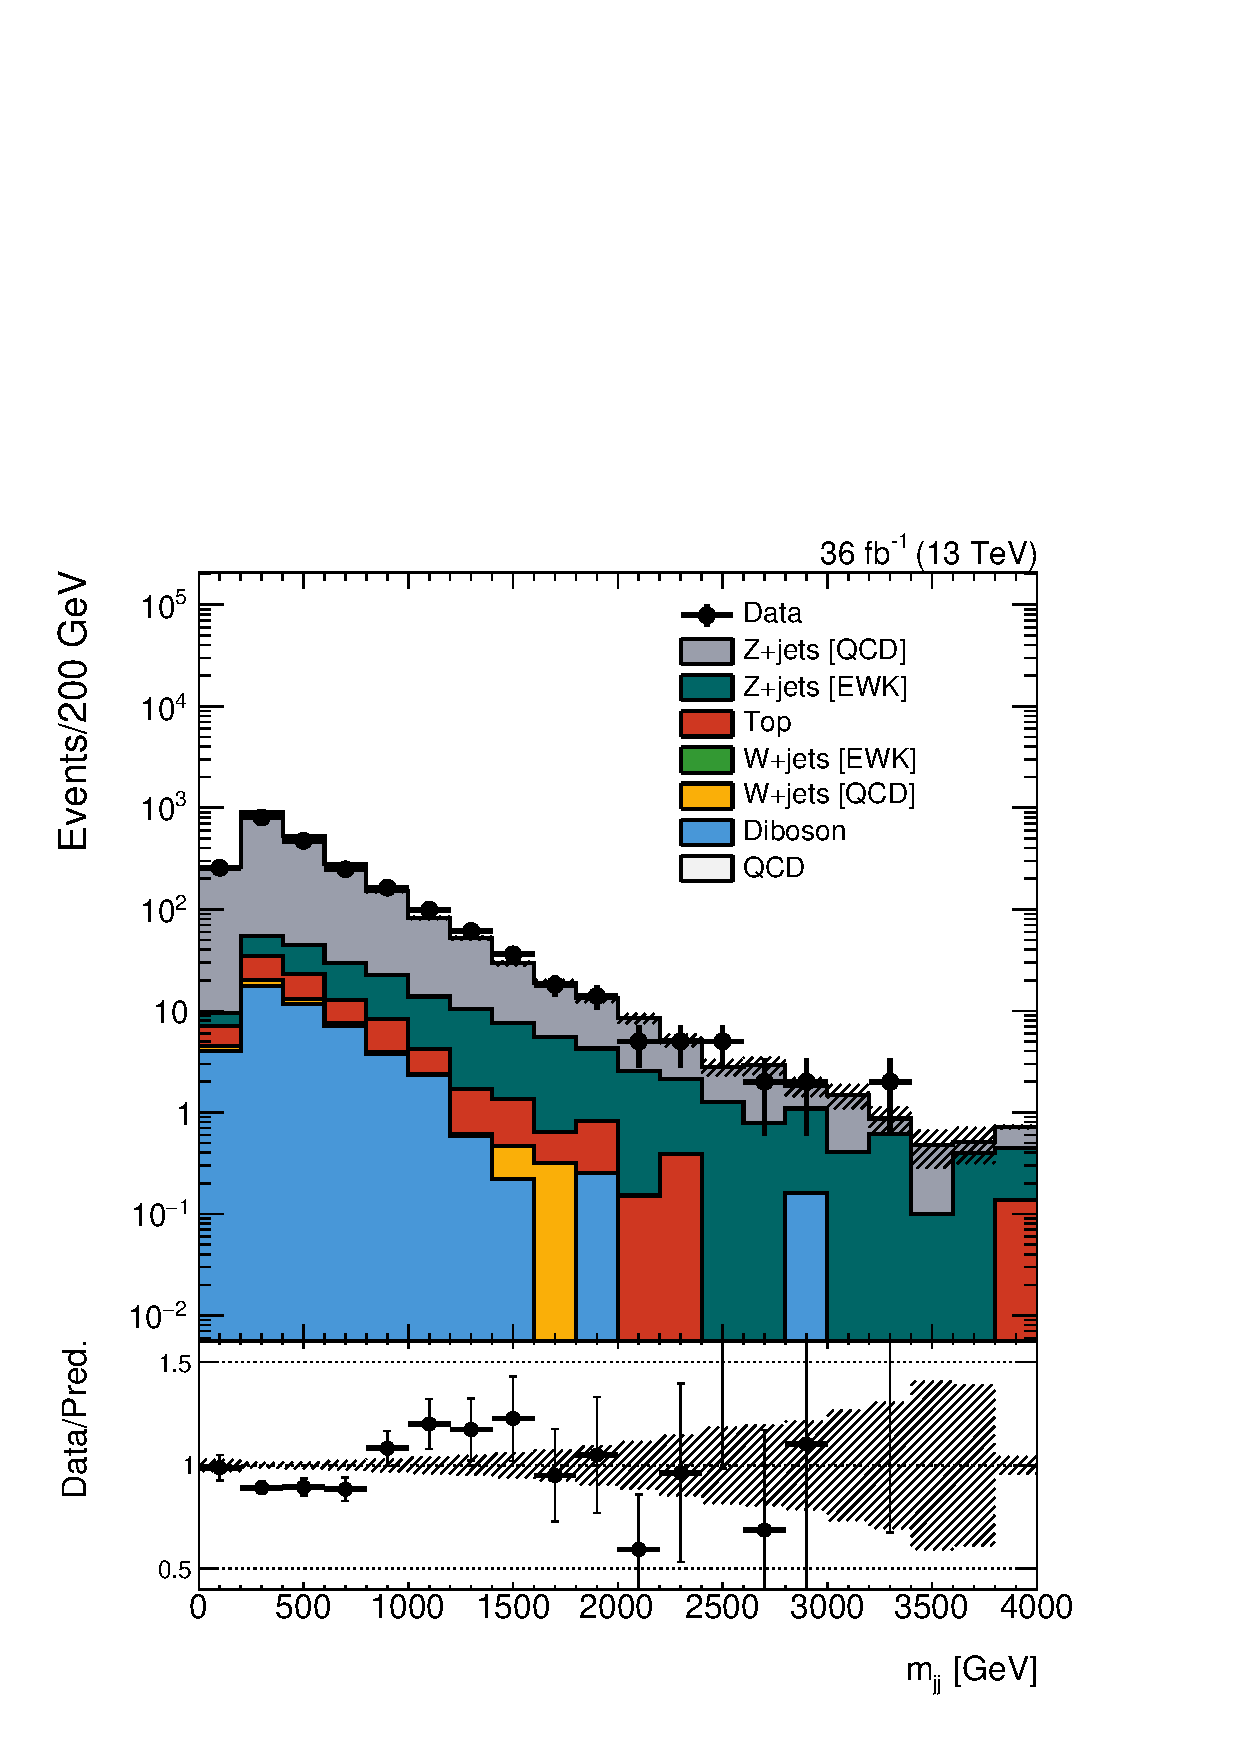
\includegraphics[width=\textwidth]{figures/vbf/prefit/dielectron_jot12Mass_logy.pdf}
        \end{subfigure}
        \begin{subfigure}[t]{0.24\textwidth}
            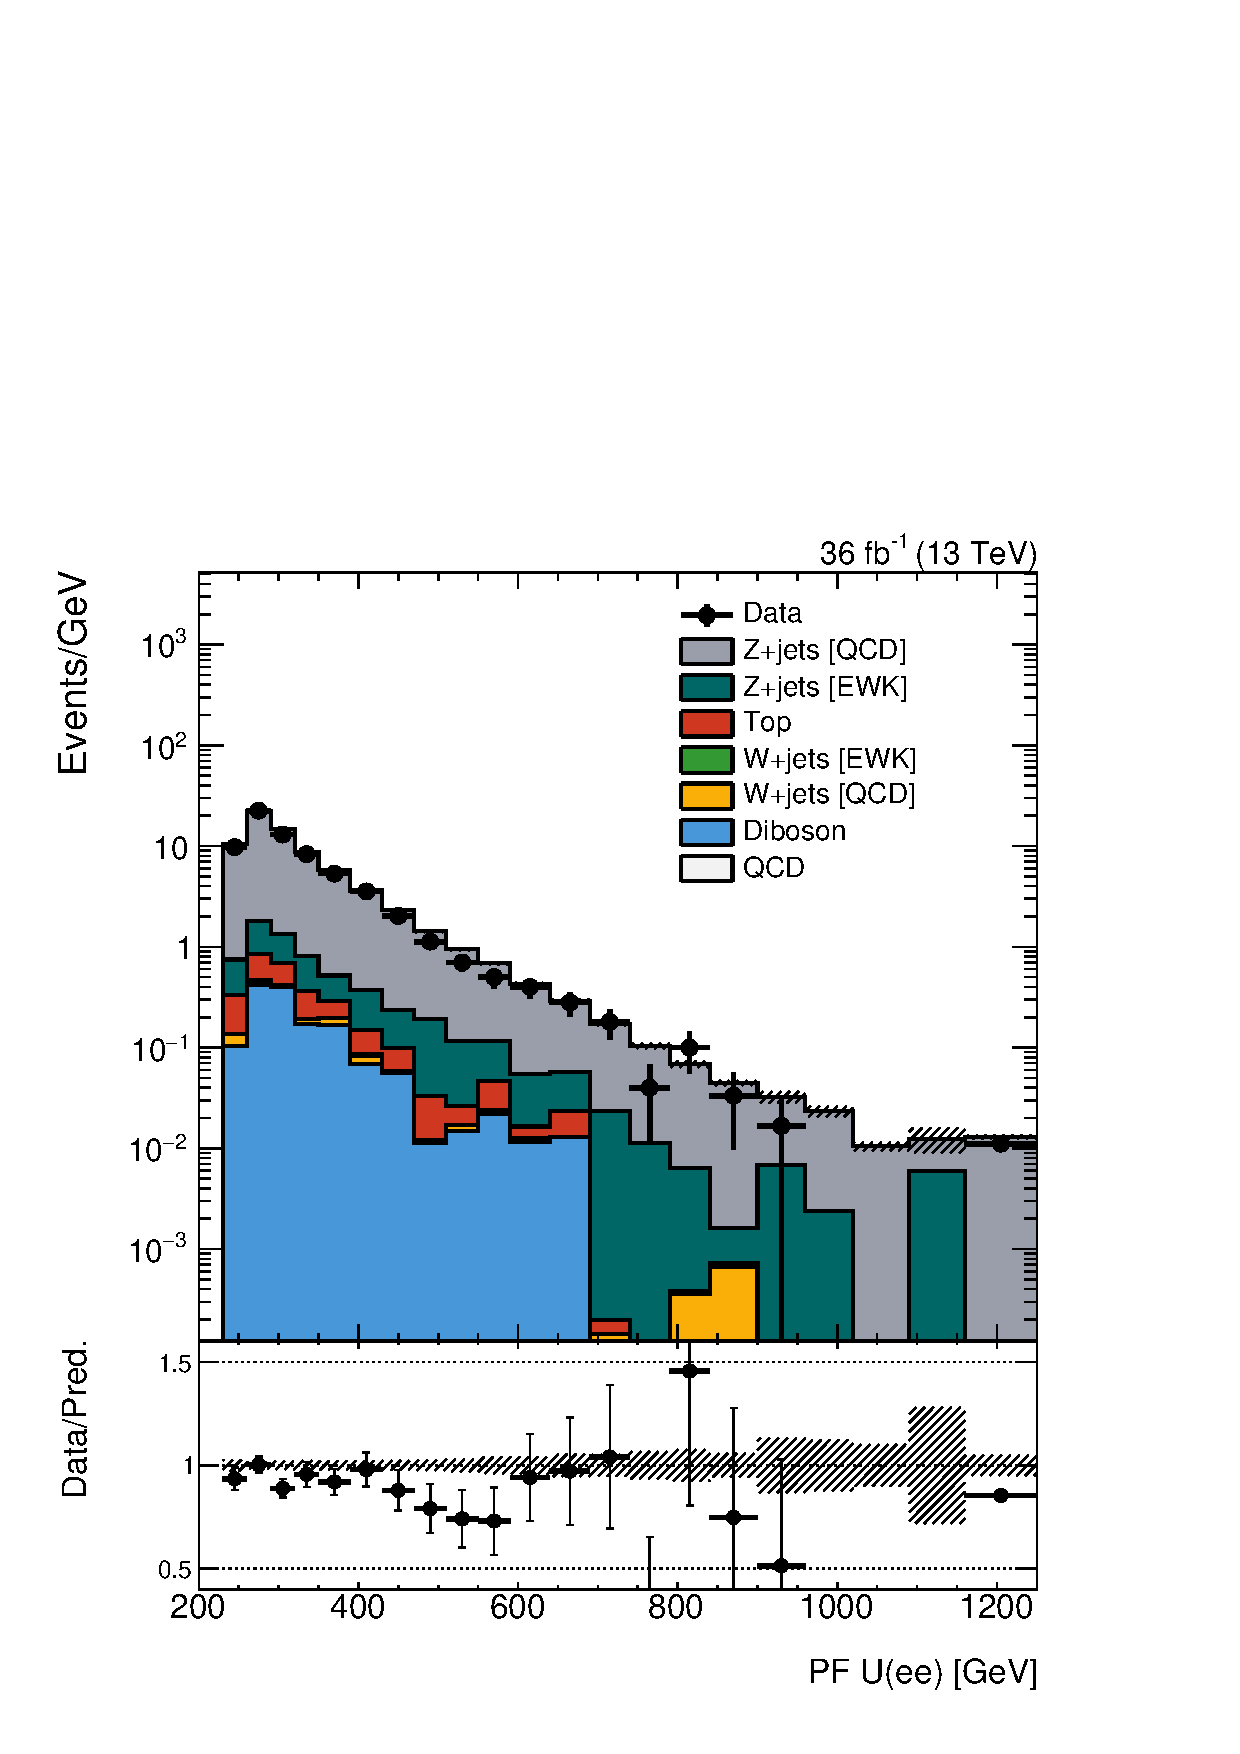
\includegraphics[width=\textwidth]{figures/vbf/prefit/dielectron_pfUZmag_logy.pdf}
        \end{subfigure} \\ 
        \begin{subfigure}[t]{0.24\textwidth}
            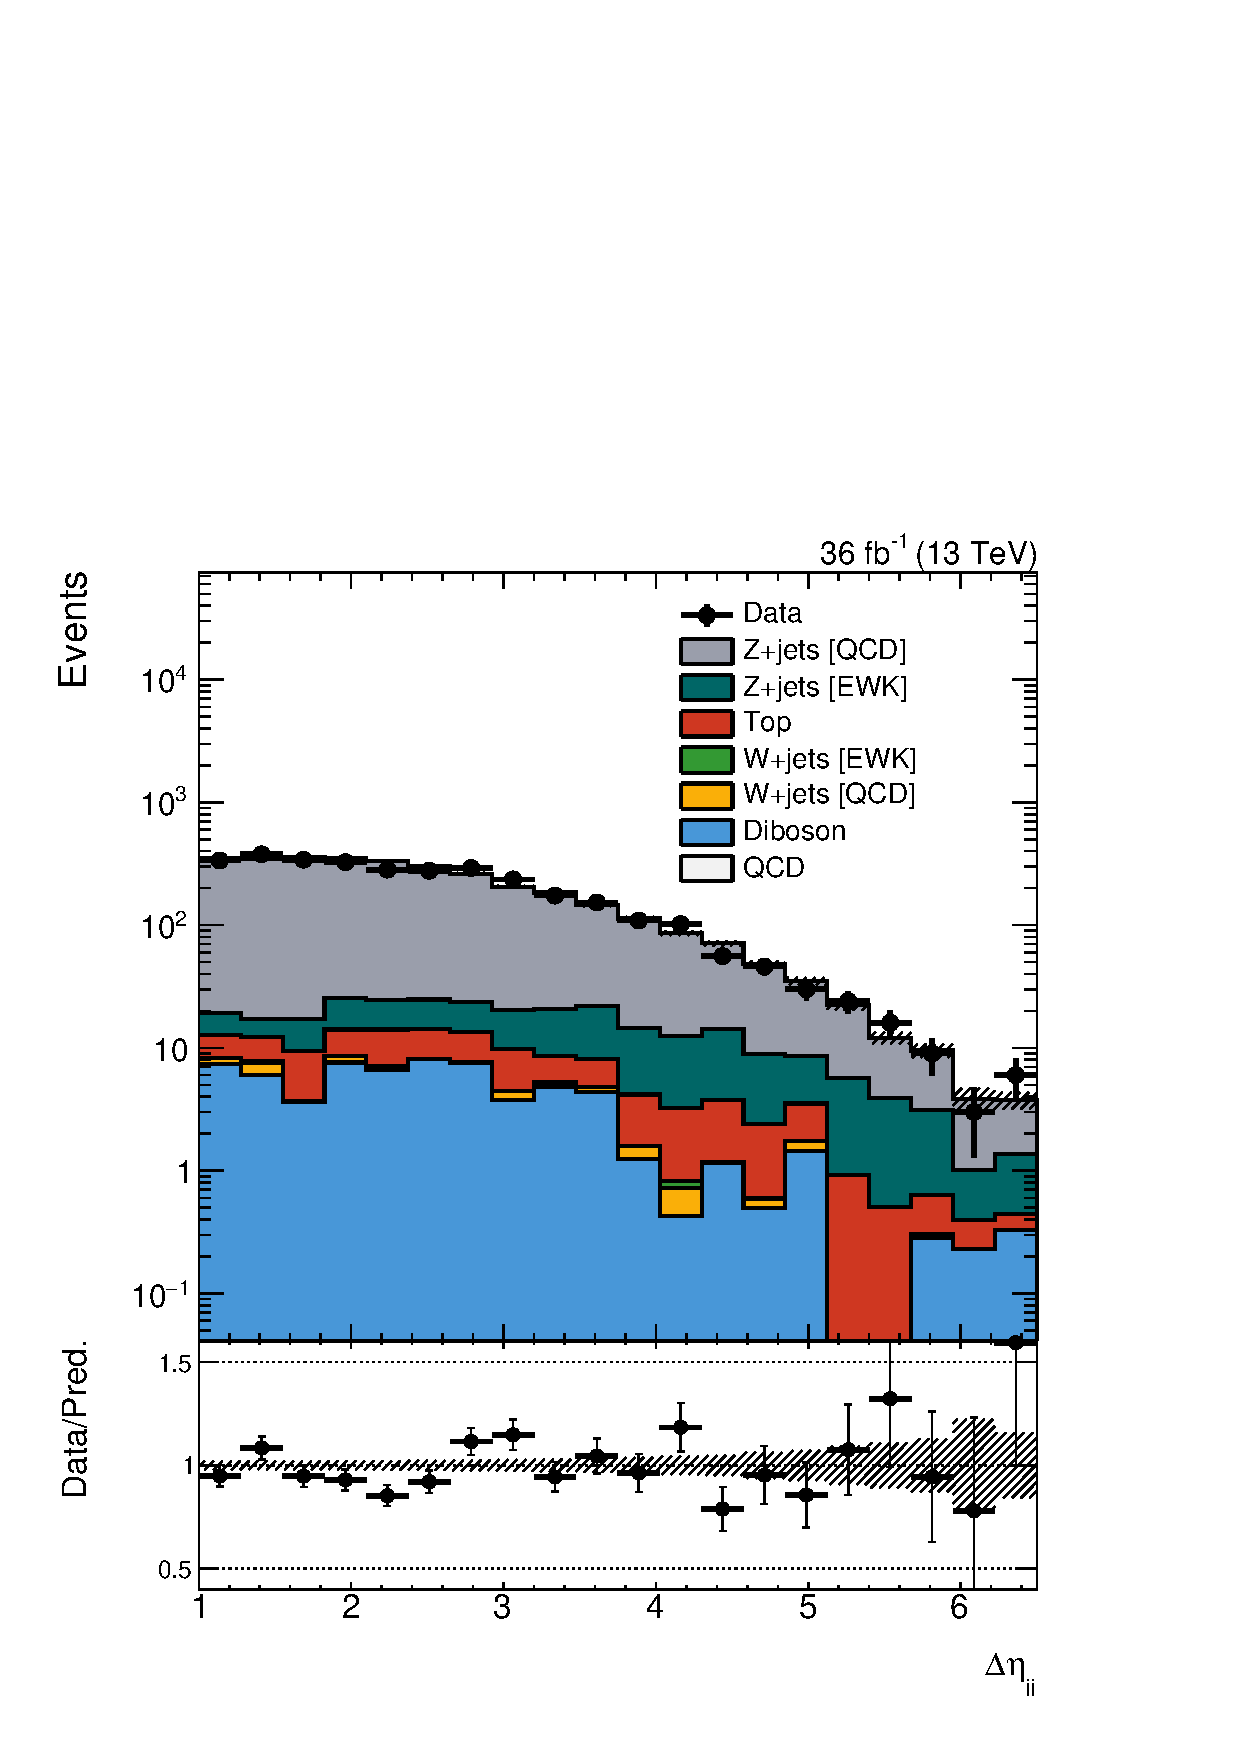
\includegraphics[width=\textwidth]{figures/vbf/prefit/dimuon_jot12DEta_logy.pdf}
        \end{subfigure}
        \begin{subfigure}[t]{0.24\textwidth}
            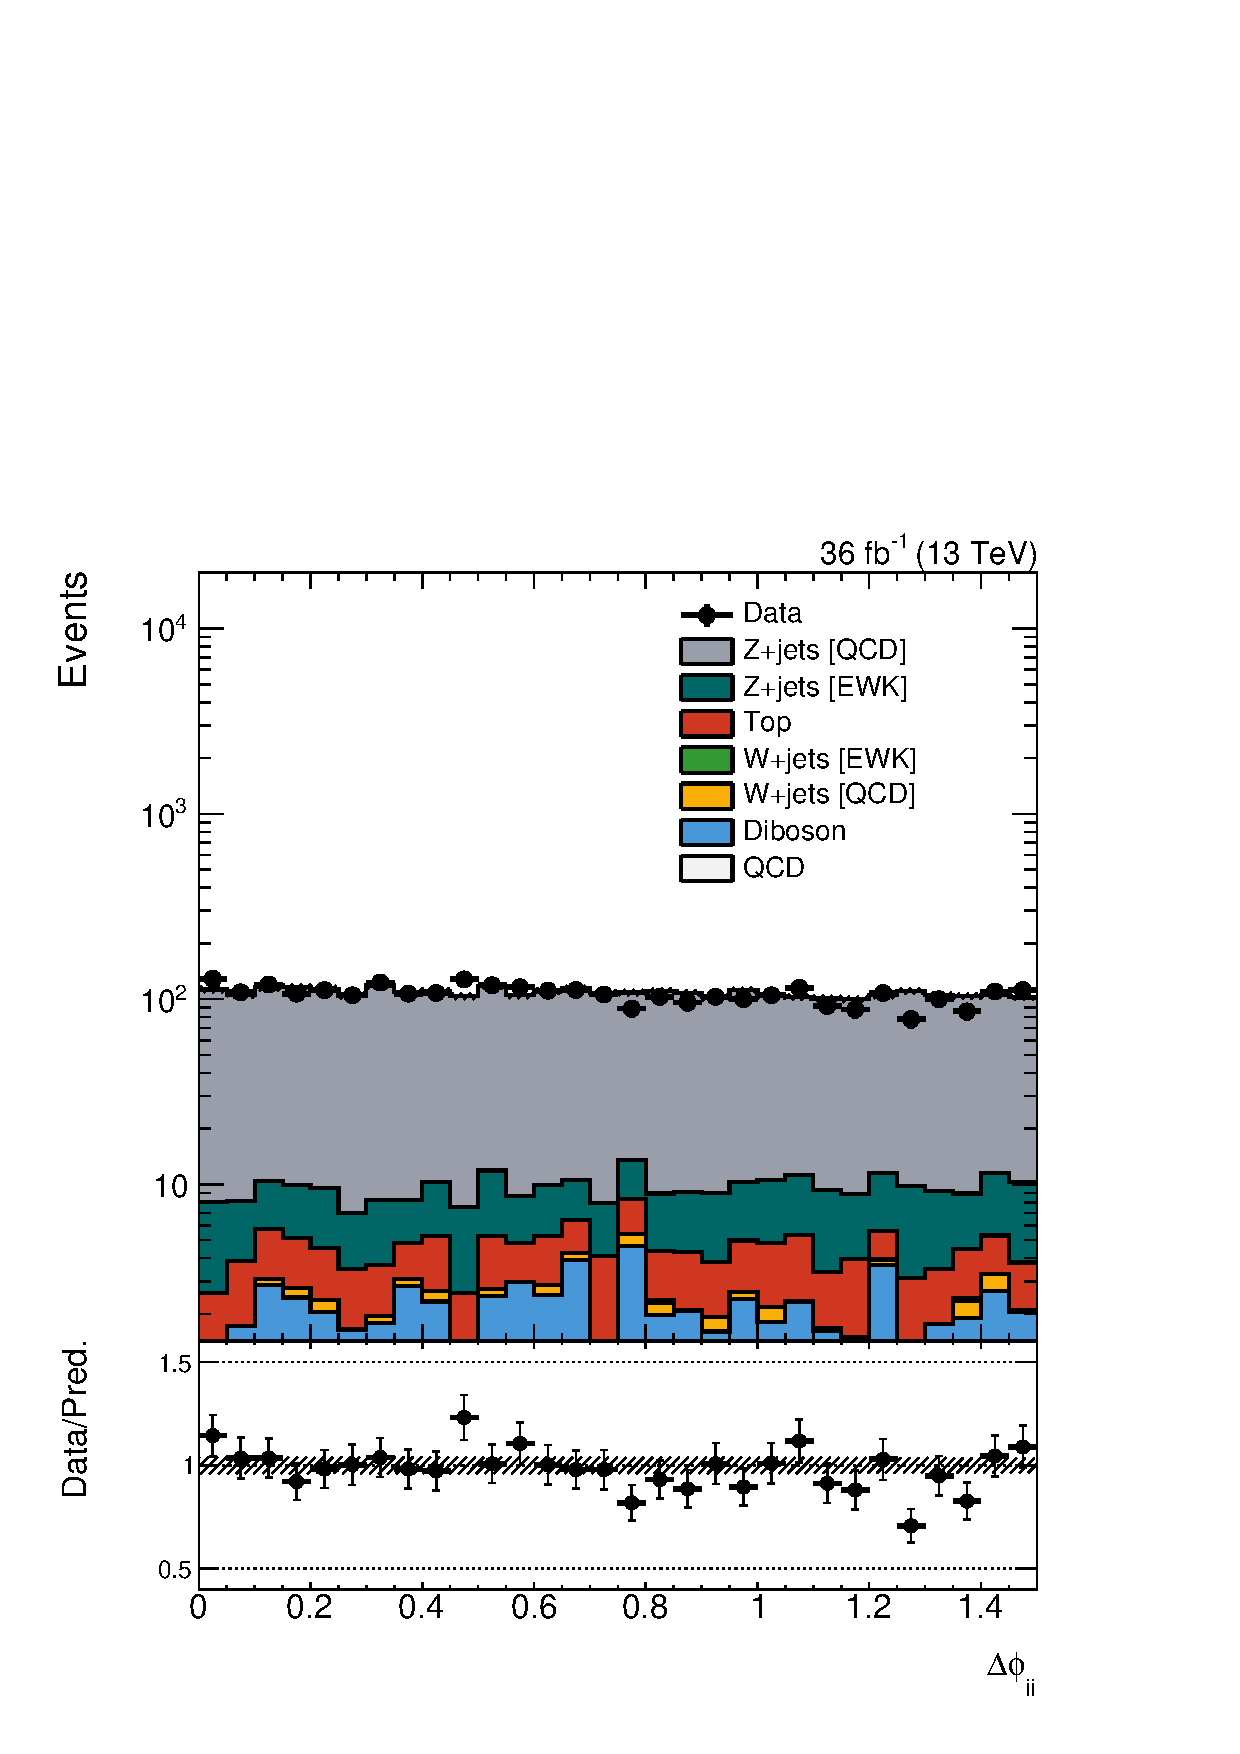
\includegraphics[width=\textwidth]{figures/vbf/prefit/dimuon_jot12DPhi_logy.pdf}
        \end{subfigure}
        \begin{subfigure}[t]{0.24\textwidth}
            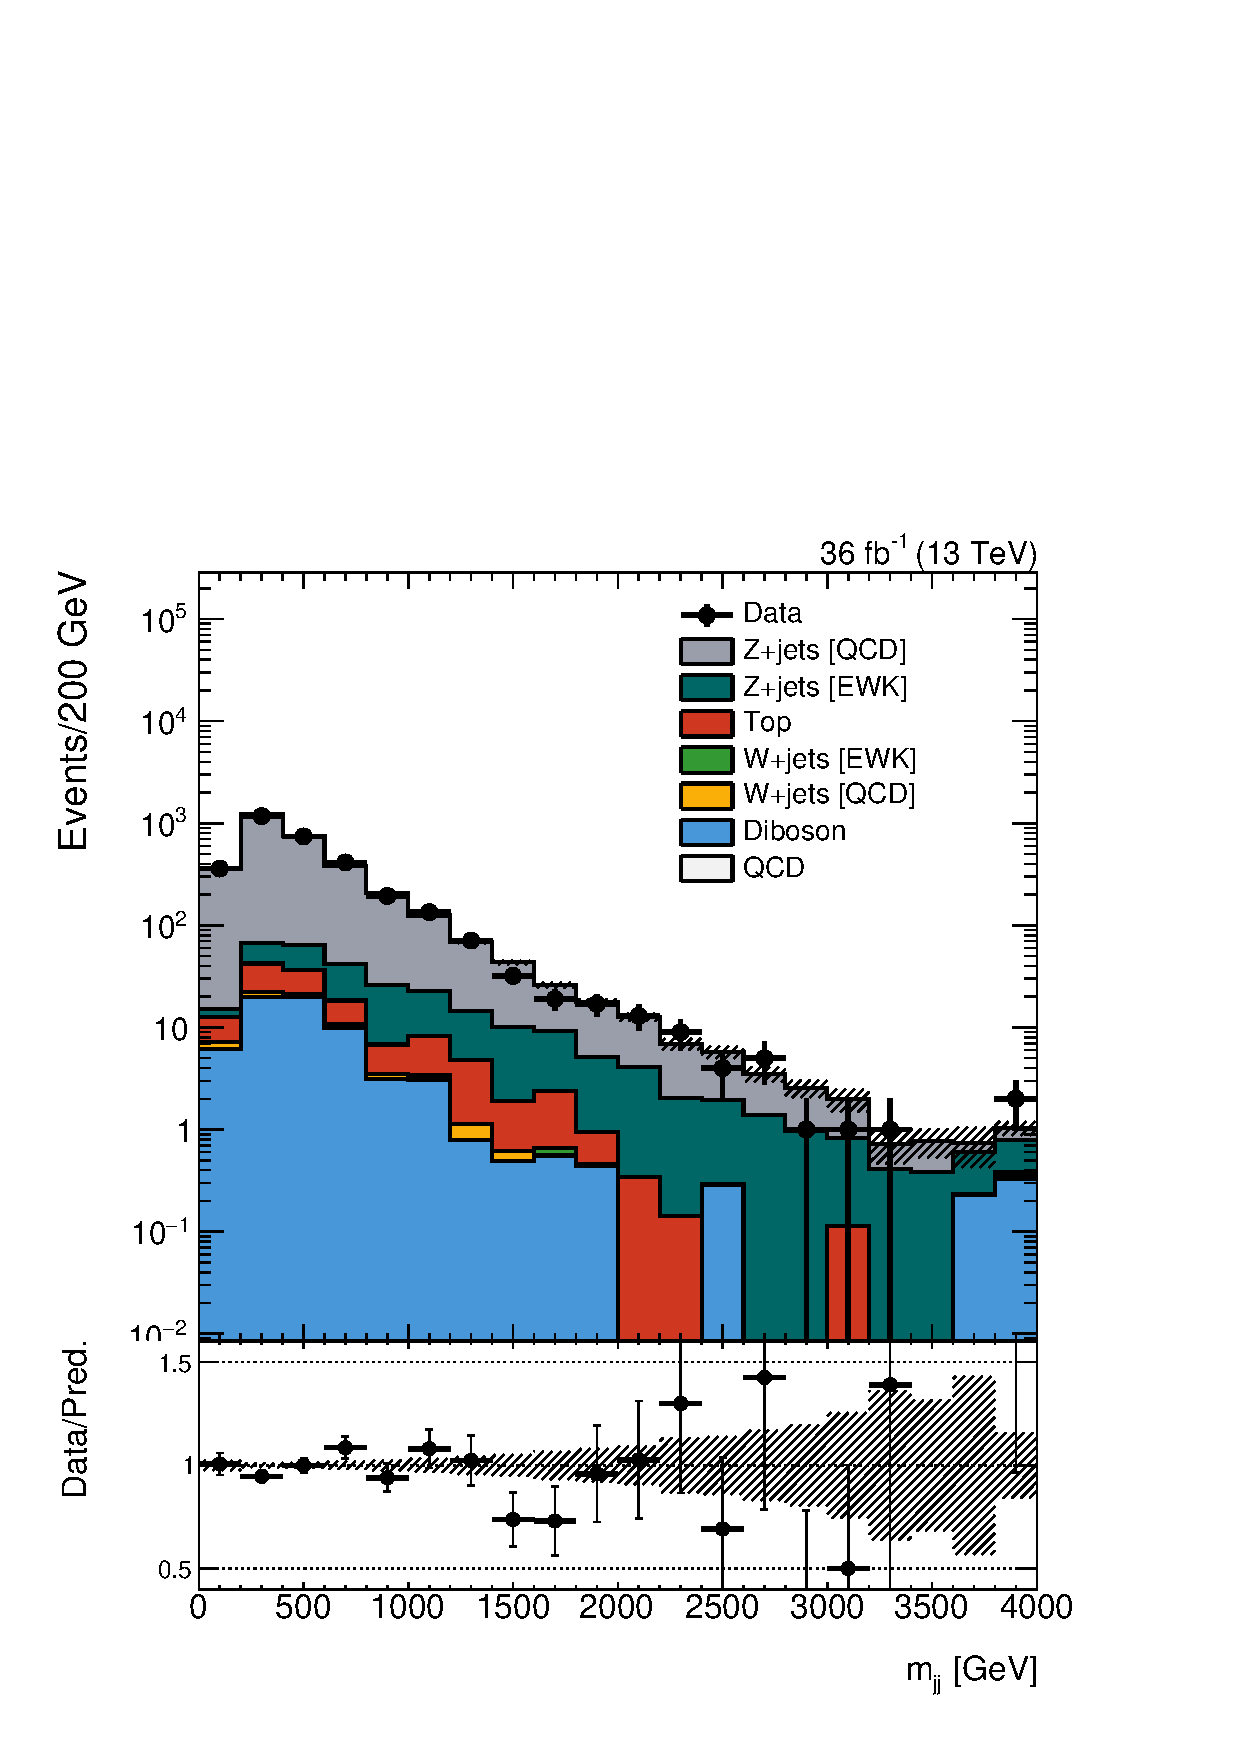
\includegraphics[width=\textwidth]{figures/vbf/prefit/dimuon_jot12Mass_logy.pdf}
        \end{subfigure}
        \begin{subfigure}[t]{0.24\textwidth}
            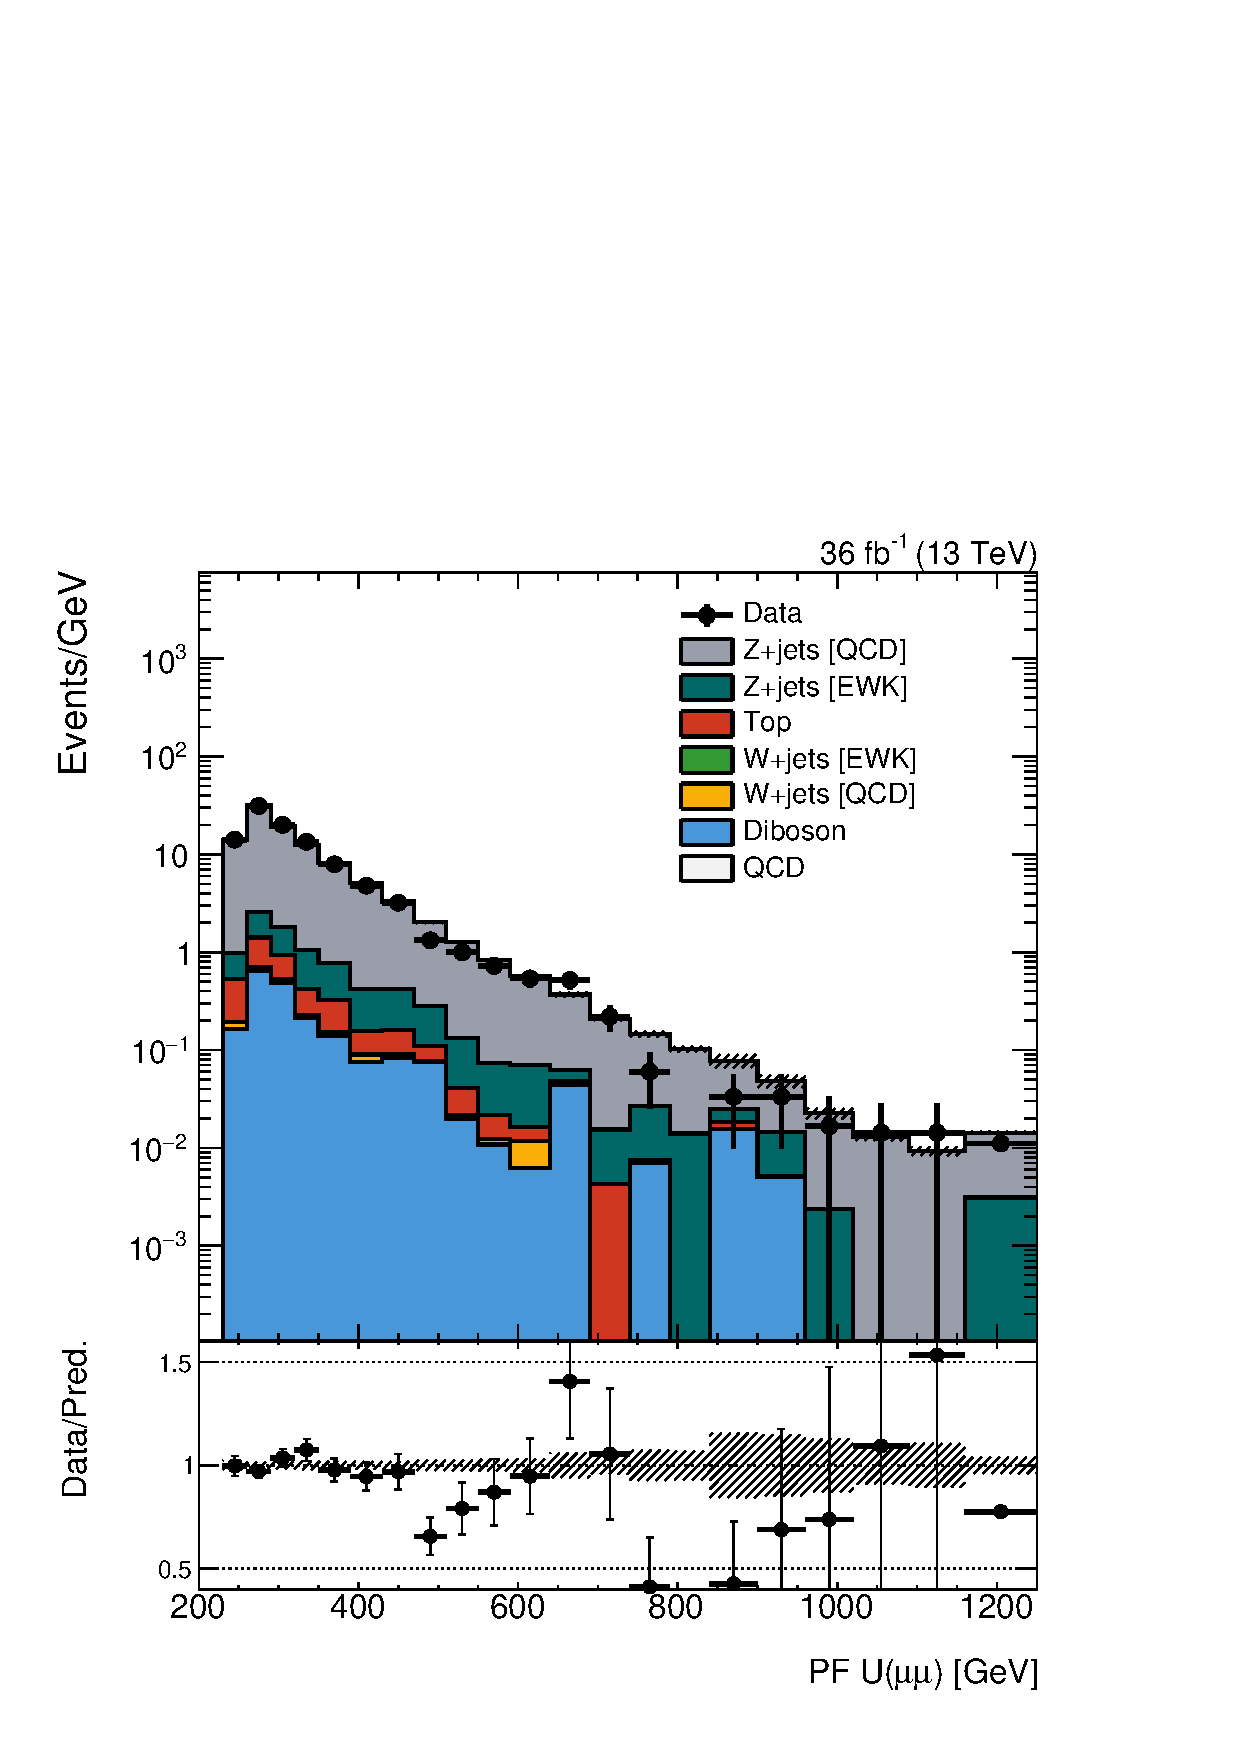
\includegraphics[width=\textwidth]{figures/vbf/prefit/dimuon_pfUZmag_logy.pdf}
        \end{subfigure}
        \caption{Dijet and recoil distributions in the dielectron (top) and dimuon (bottom) CRs.}
        \label{fig:vbf:zcr}
    \end{center}
\end{figure}

In the region $m_{jj}>2.5$ TeV, the statistical power of the dilepton regions is extremely limited.
For this reason, and to estimate the $W$+jets contribution in the SR, we add two single-lepton CRs in analogy to what is done in Section~\ref{sec:mt:bkg}. 
Figure~\ref{fig:vbf:wcr} shows the level of agreement between the data and MC in these CRs.
The likelihood is modified to include the constraints of the single-lepton CRs:
\begin{align}
    \mathcal{L}\left(\bm{d}\,|\, \mu,\muz,\bm{\theta}\right) = \hspace{-30mm} & \nonumber \\
    \prod_{i\in\mathrm{bins}} & \left[
    \pois\left\{d^{\mathrm{SR}}_{i} ~\Big|~ \mu S^{\mathrm{SR}}_{i}(\bm\theta)  + \left(1+\frac{1}{\Ti{\mathrm{QE}}{Z}(\bm\theta)}\right)\left(1+\frac{1}{\Ti{\mathrm{SR}}{Z/W}(\bm\theta)}\right)\muzi + B^{\mathrm{SR}}_{i}(\bm\theta)\right\} \vphantom{\frac{\muzi}{\Ti{\mu\mu}{Z}(\bm\theta)}}\right. \nonumber \\
    & \phantom{\Big[} \times \prod_{X=\mu,e} \pois\left\{d^{X}_i~\Big|~ \left(1+\frac{1}{\Ti{\mathrm{QE}}{Z}(\bm\theta)}\right)\frac{\muzi}{\Ti{X}{W}(\bm\theta)\Ti{\mathrm{SR}}{Z/W}(\bm\theta)} + B^{X}_i(\bm\theta) \right\} \nonumber \\
    & \phantom{\Big[} \times \left.\prod_{X=\mu\mu,ee} \pois\left\{d^{X}_i~\Big|~ \left(1+\frac{1}{\Ti{\mathrm{QE}}{Z}(\bm\theta)}\right)\frac{\muzi}{\Ti{X}{Z}(\bm\theta)} + B^{X}_i(\bm\theta) \right\} \right]  \times  \prod_{j=0}^{n_\theta} p_j(\theta_j)
\end{align}
To validate that the transfer factors are reasonably well-simulated (within the assigned uncertainties), Figure~\ref{fig:vbf:valid} uses the following ratios of CRs as proxies for transfer factors:
\begin{gather}
    \T{\mu\mu}{Z}, \T{ee}{Z} \sim \frac{N_{\mu\mu}(Z\rightarrow\mu\mu)}{N_{ee}(Z\rightarrow ee)} \nonumber \\ 
    \T{\mu}{W}, \T{e}{W} \sim \frac{N_\mu(W\rightarrow\mu\nu)}{N_e(W\rightarrow e\nu)} \nonumber \\ 
    \T{\mathrm{SR}}{Z/W} \sim \frac{N_\mu(W\rightarrow\mu\nu)+N_e(W\rightarrow e\nu)}{N_{\mu\mu}(Z\rightarrow\mu\mu)+N_{ee}(Z\rightarrow ee)} 
\end{gather}

\begin{figure}[]
    \begin{center}
        \begin{subfigure}[t]{0.24\textwidth}
            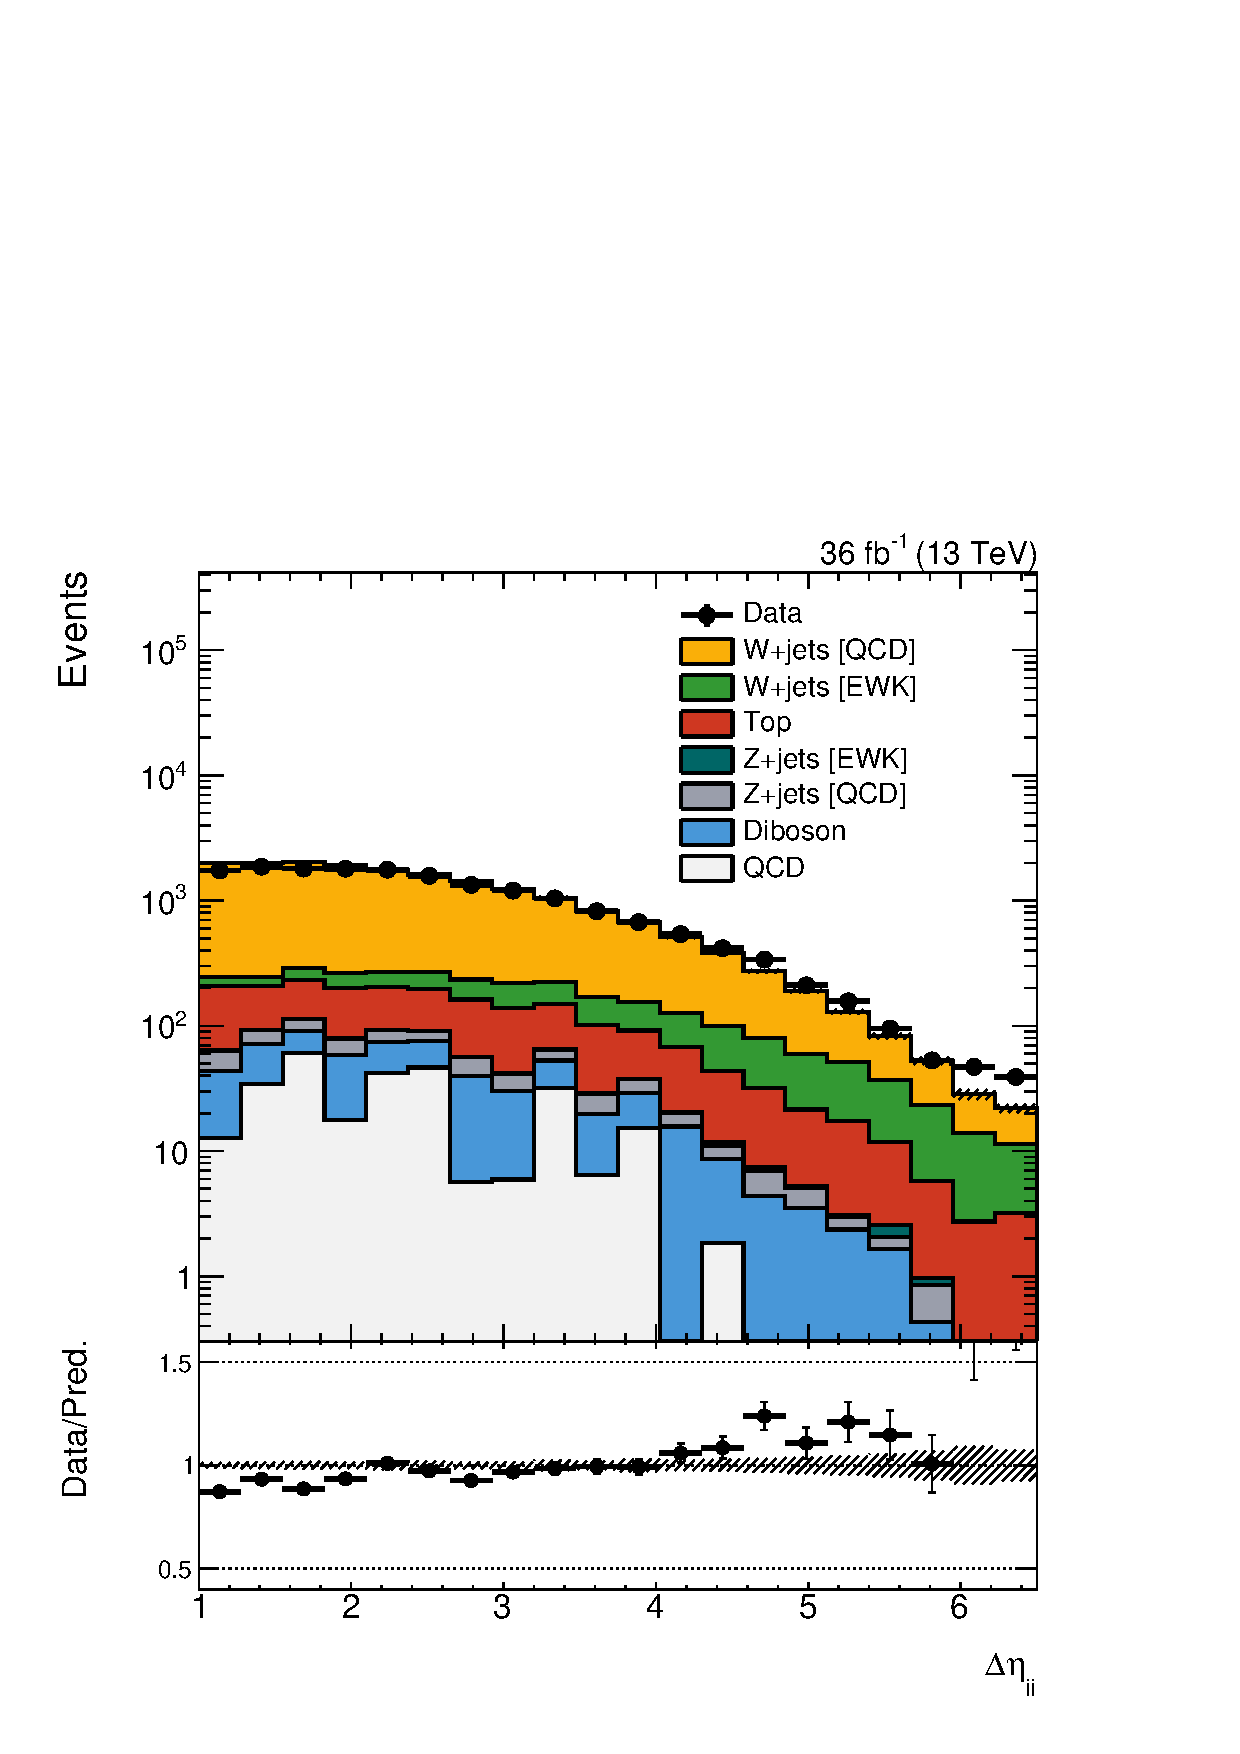
\includegraphics[width=\textwidth]{figures/vbf/prefit/singleelectron_jot12DEta_logy.pdf}
        \end{subfigure}
        \begin{subfigure}[t]{0.24\textwidth}
            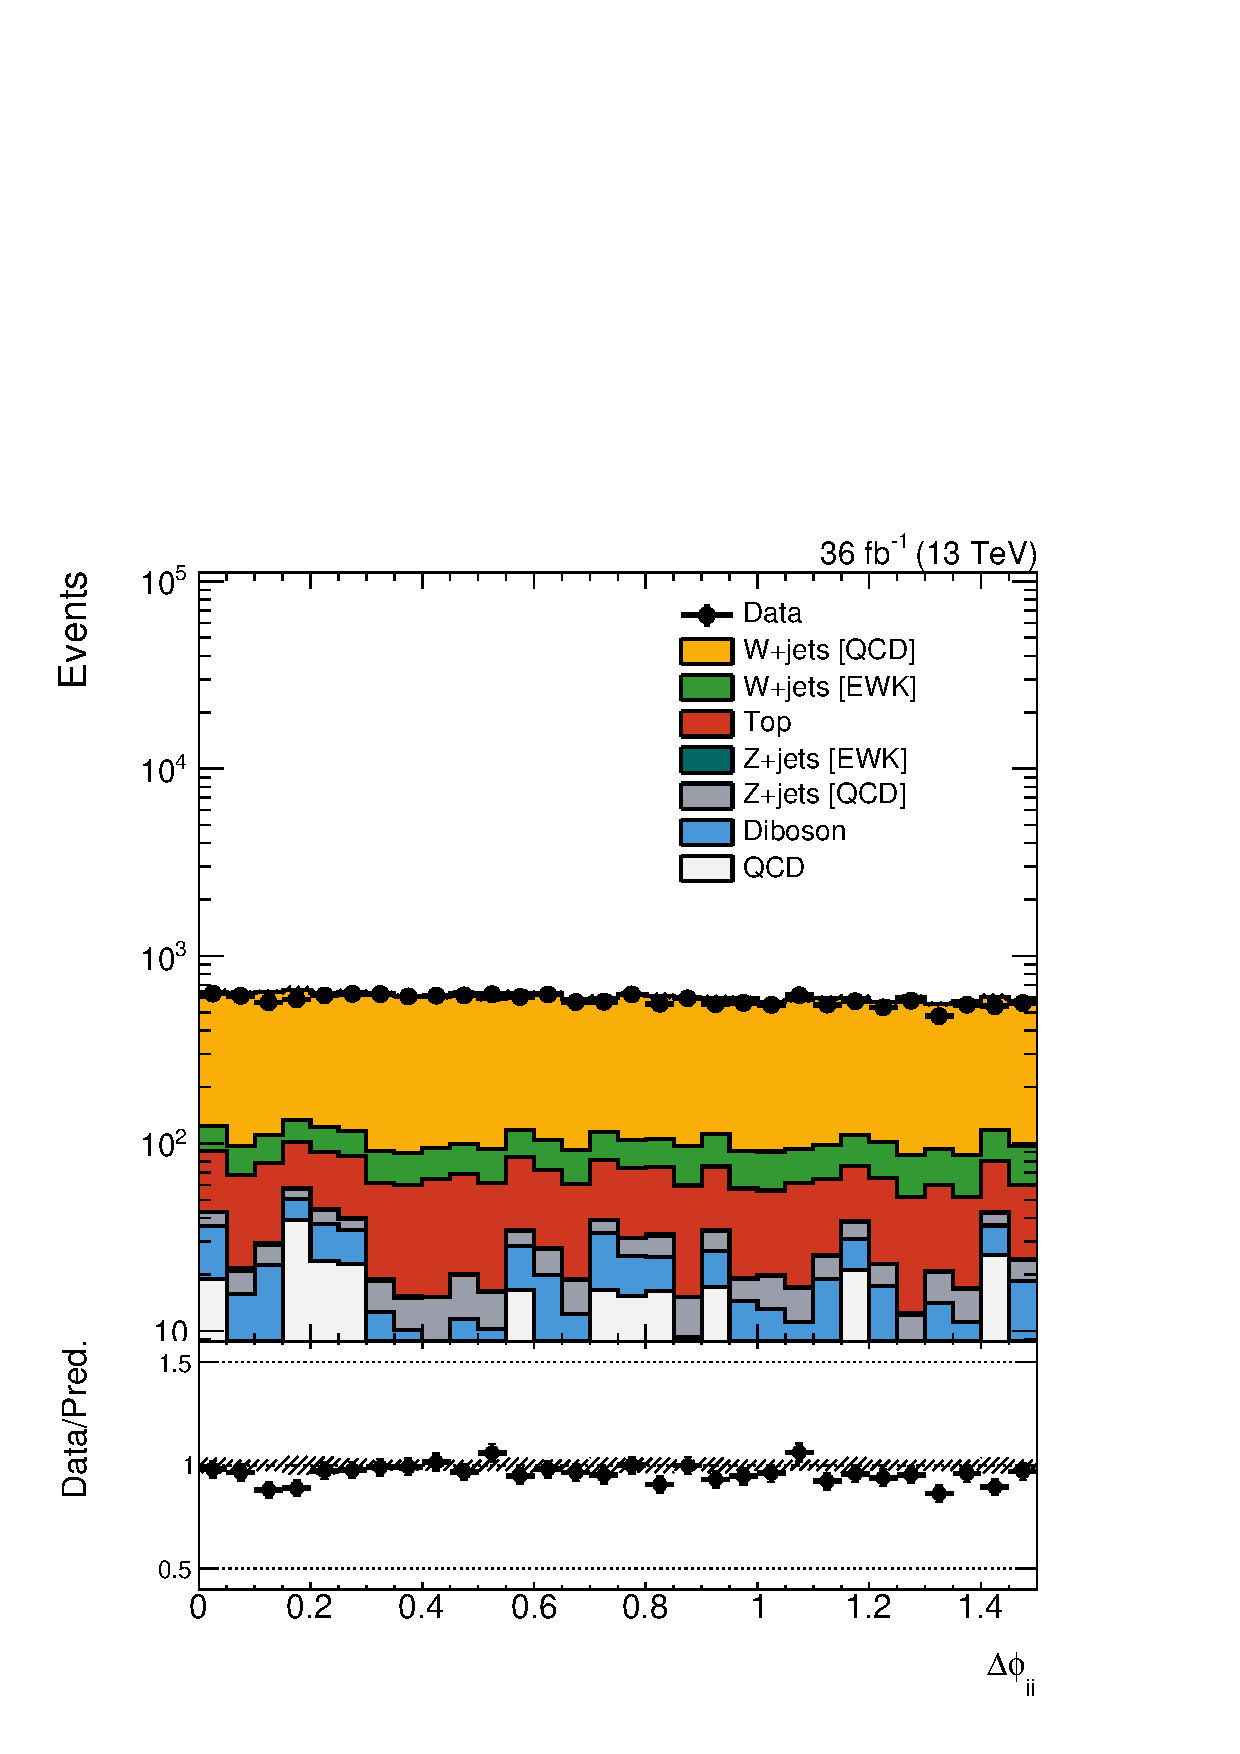
\includegraphics[width=\textwidth]{figures/vbf/prefit/singleelectron_jot12DPhi_logy.pdf}
        \end{subfigure}
        \begin{subfigure}[t]{0.24\textwidth}
            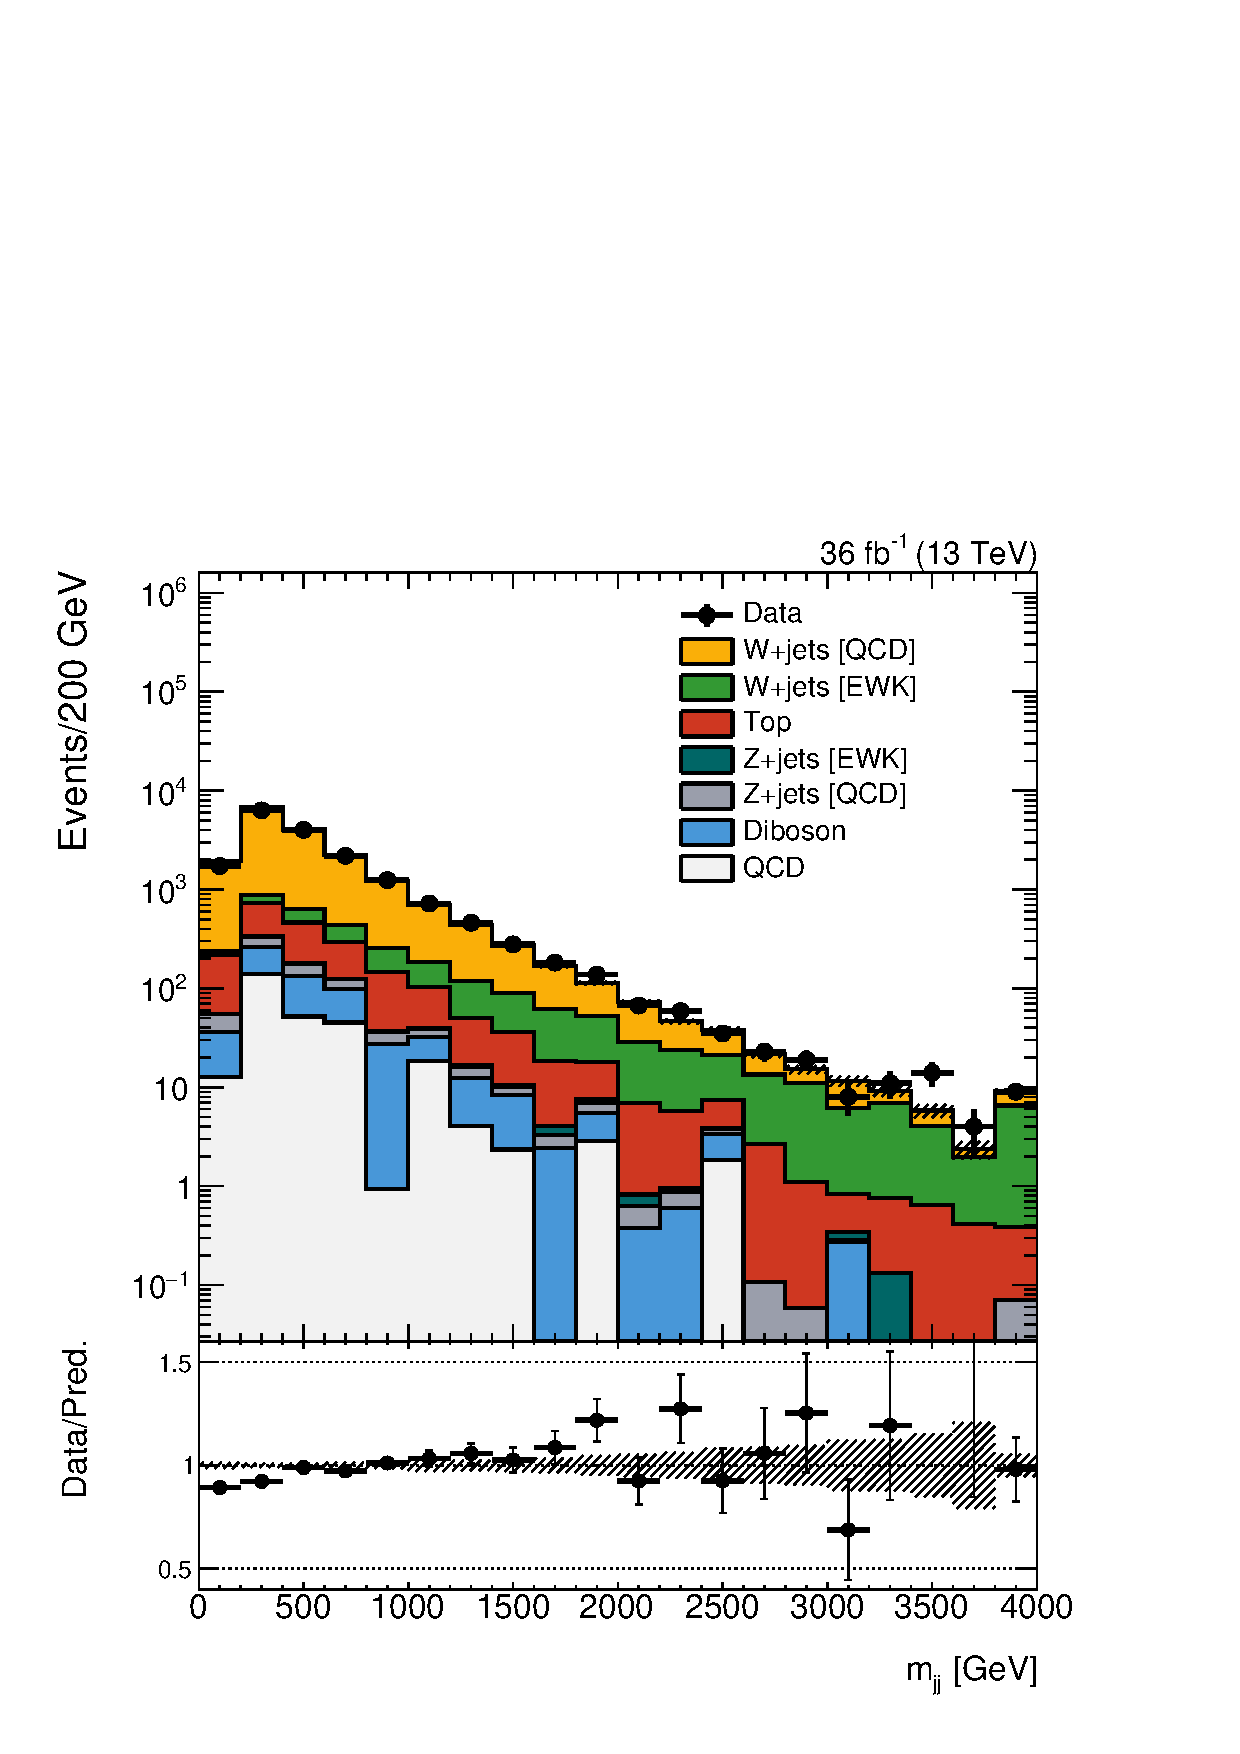
\includegraphics[width=\textwidth]{figures/vbf/prefit/singleelectron_jot12Mass_logy.pdf}
        \end{subfigure}
        \begin{subfigure}[t]{0.24\textwidth}
            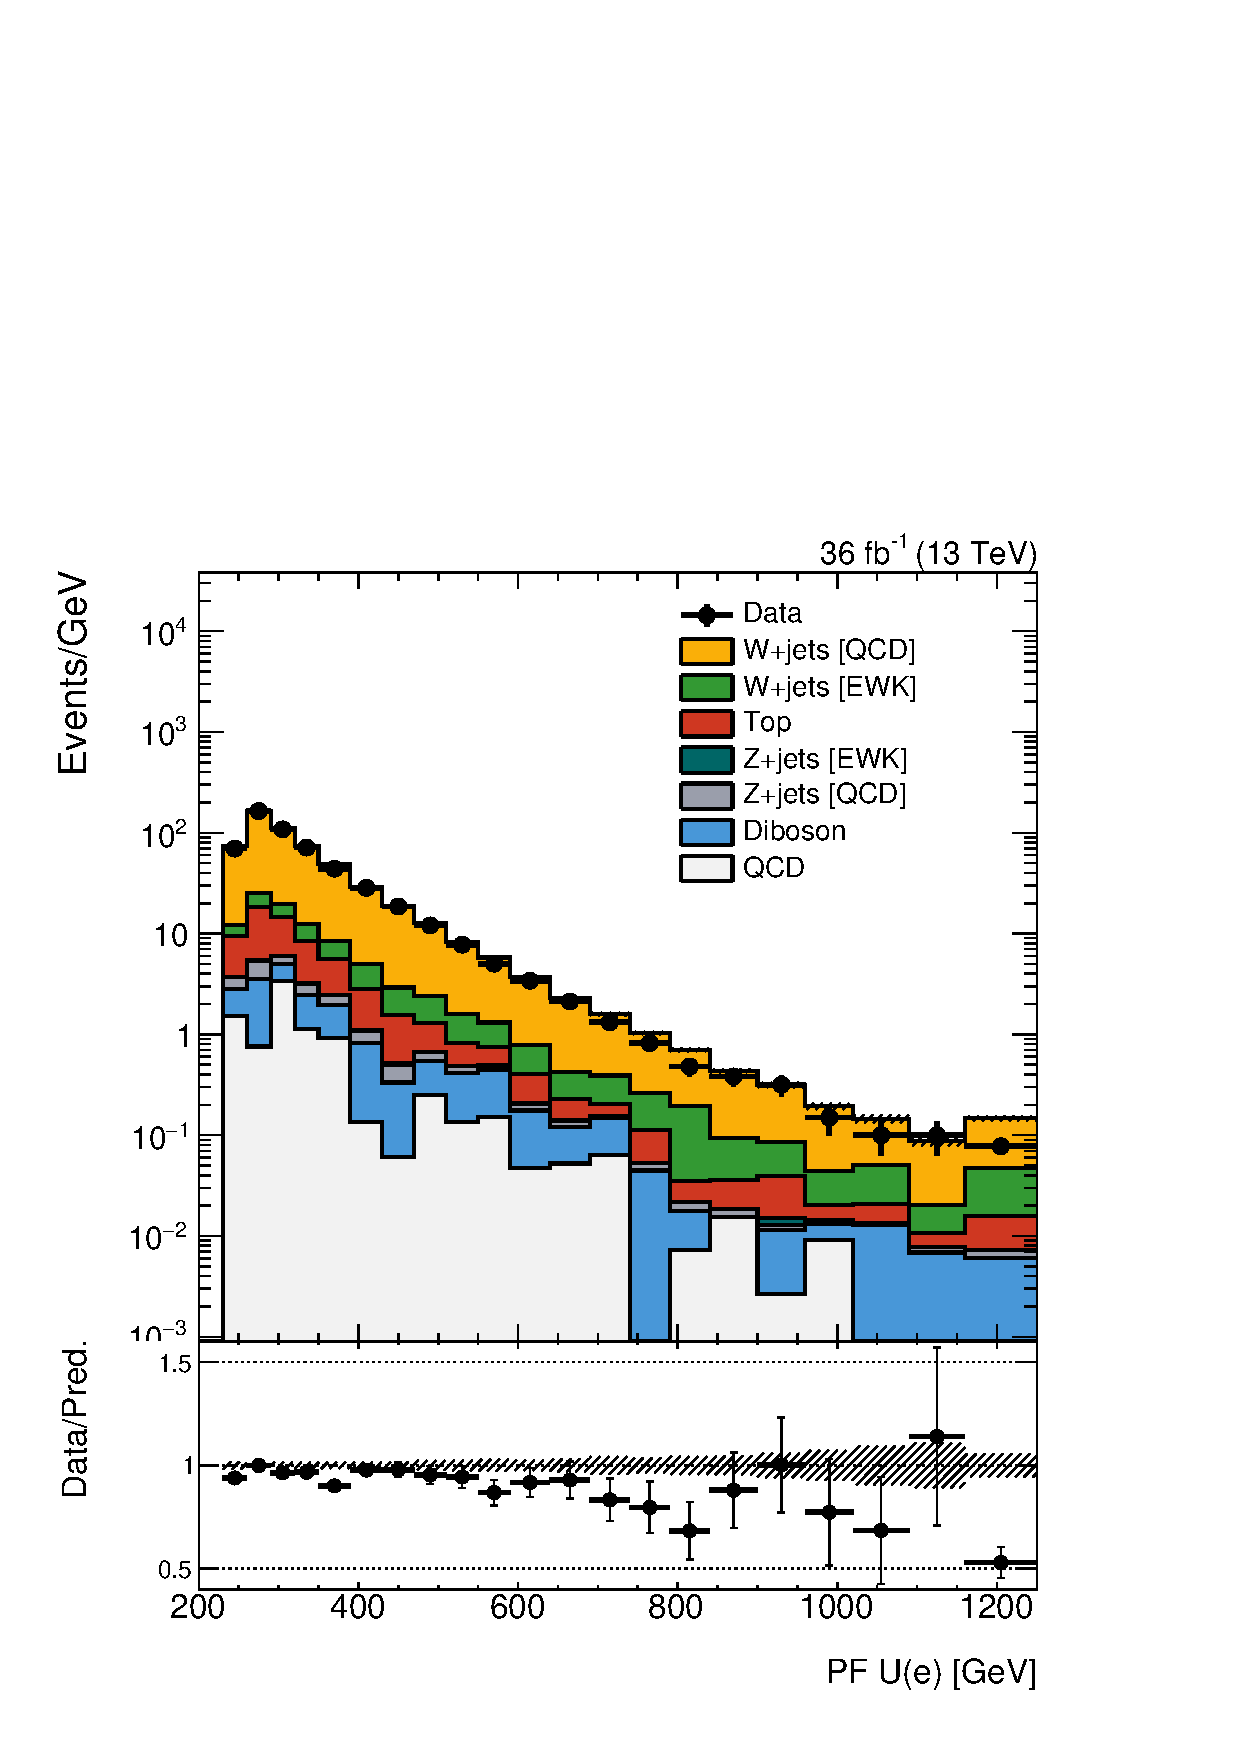
\includegraphics[width=\textwidth]{figures/vbf/prefit/singleelectron_pfUWmag_logy.pdf}
        \end{subfigure} \\ 
        \begin{subfigure}[t]{0.24\textwidth}
            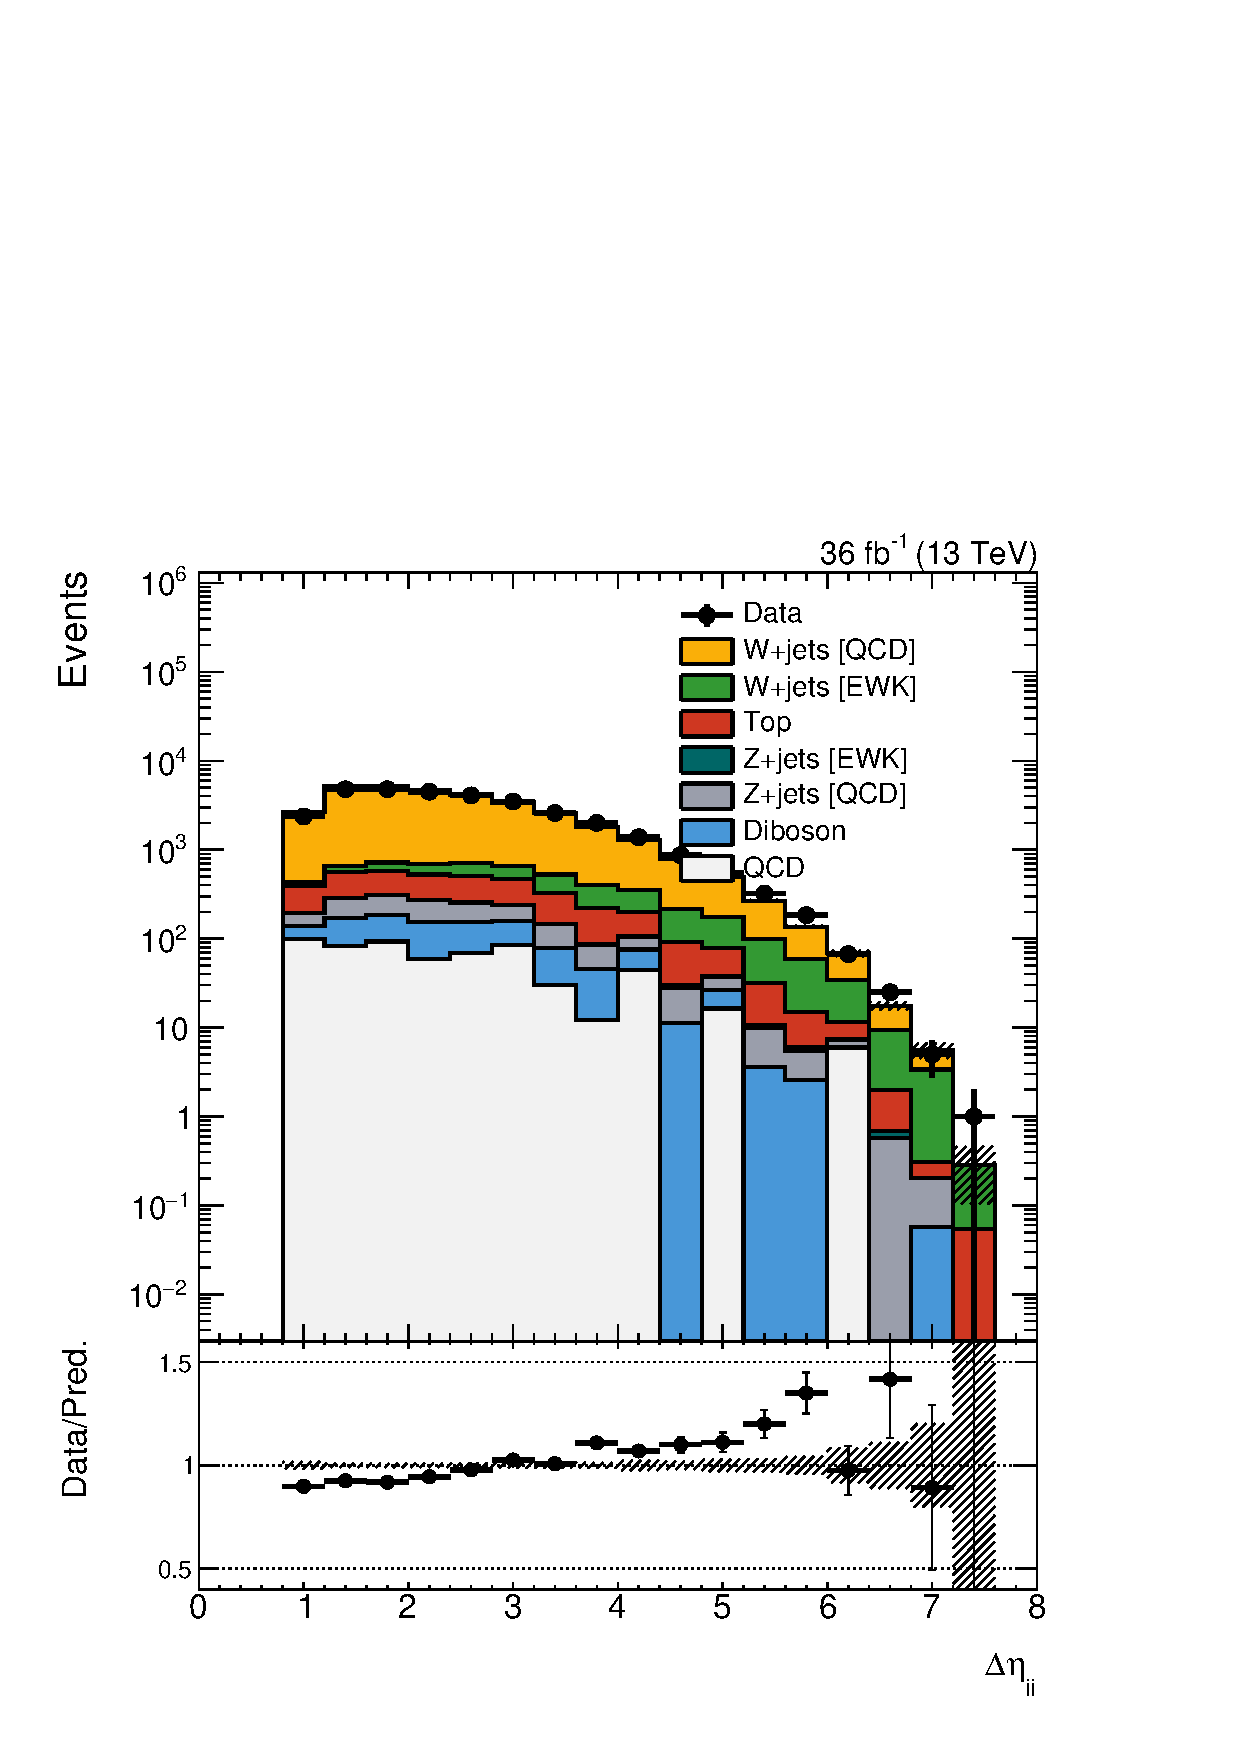
\includegraphics[width=\textwidth]{figures/vbf/prefit/singlemuon_jot12DEta_logy.pdf}
        \end{subfigure}
        \begin{subfigure}[t]{0.24\textwidth}
            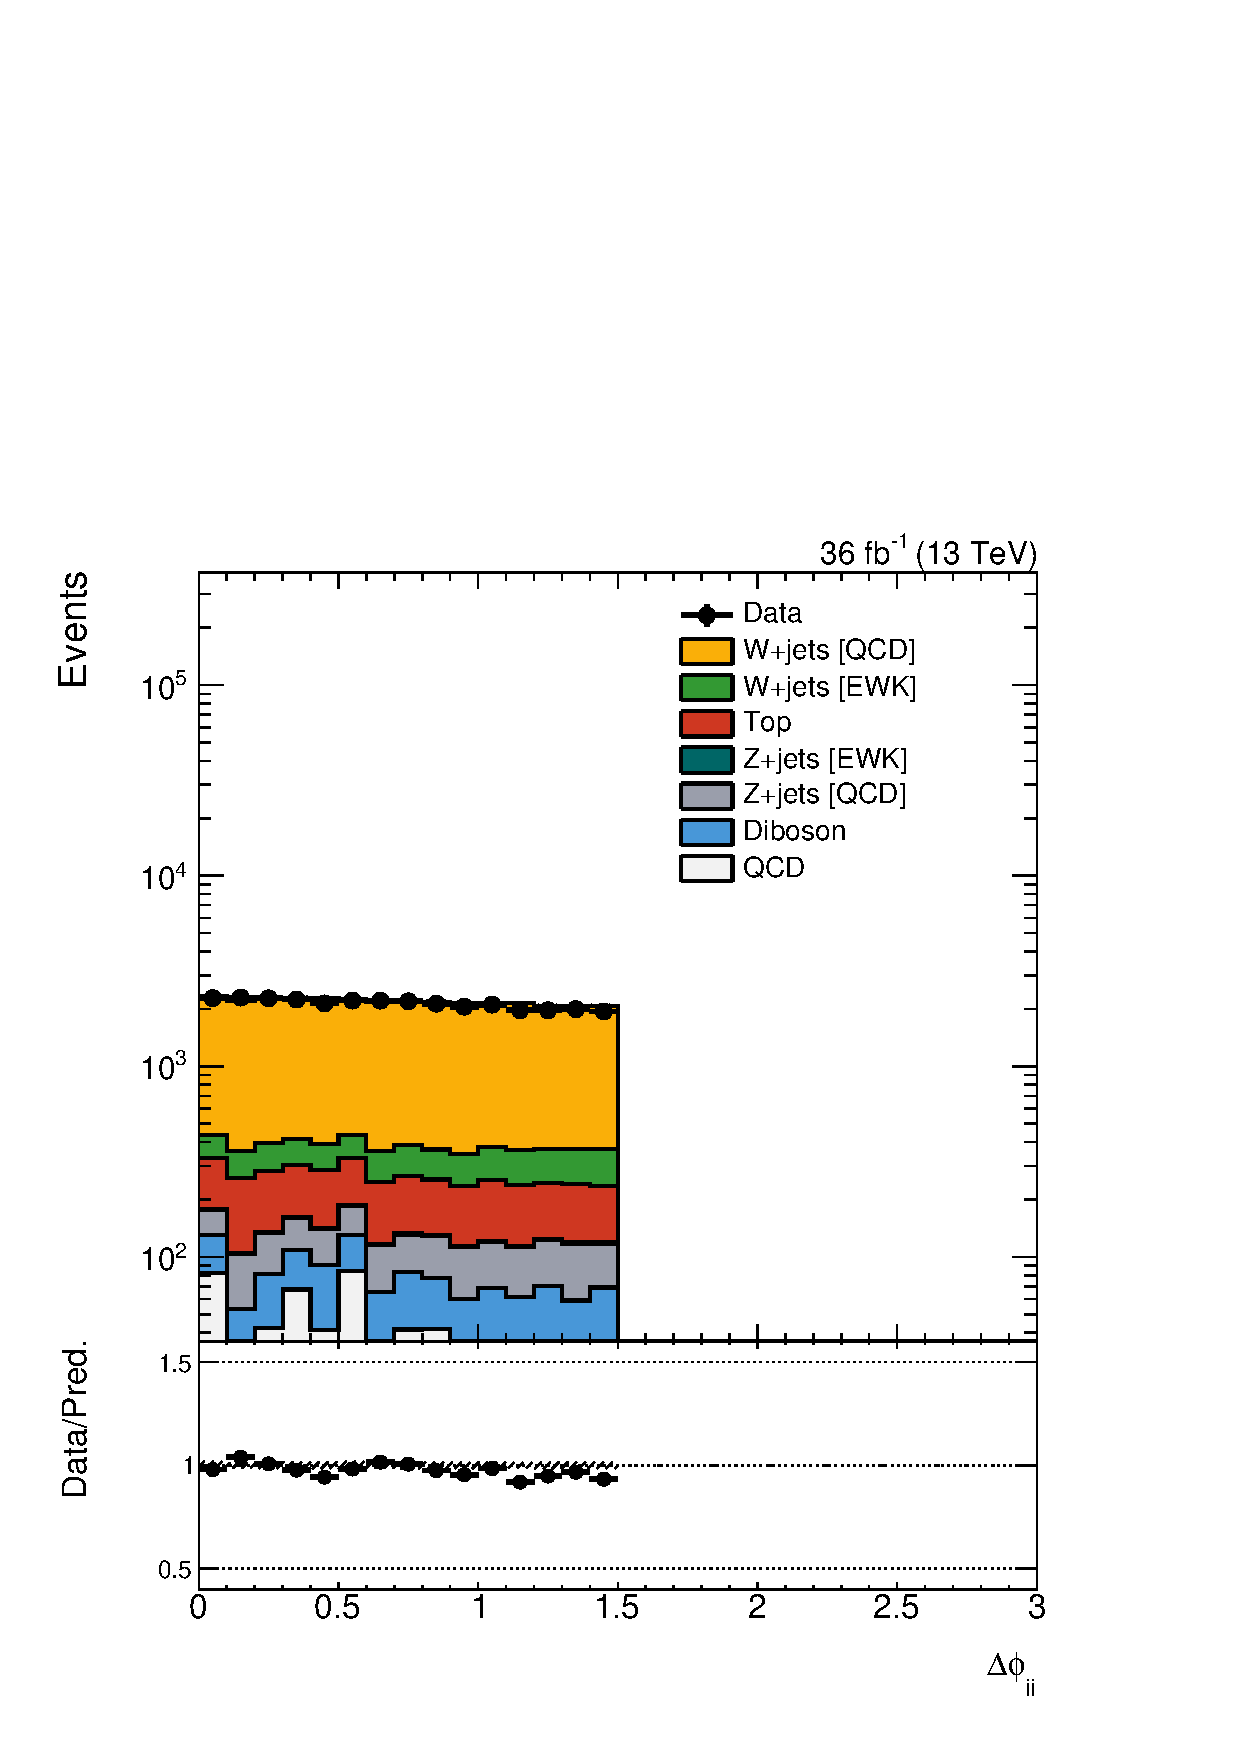
\includegraphics[width=\textwidth]{figures/vbf/prefit/singlemuon_jot12DPhi_logy.pdf}
        \end{subfigure}
        \begin{subfigure}[t]{0.24\textwidth}
            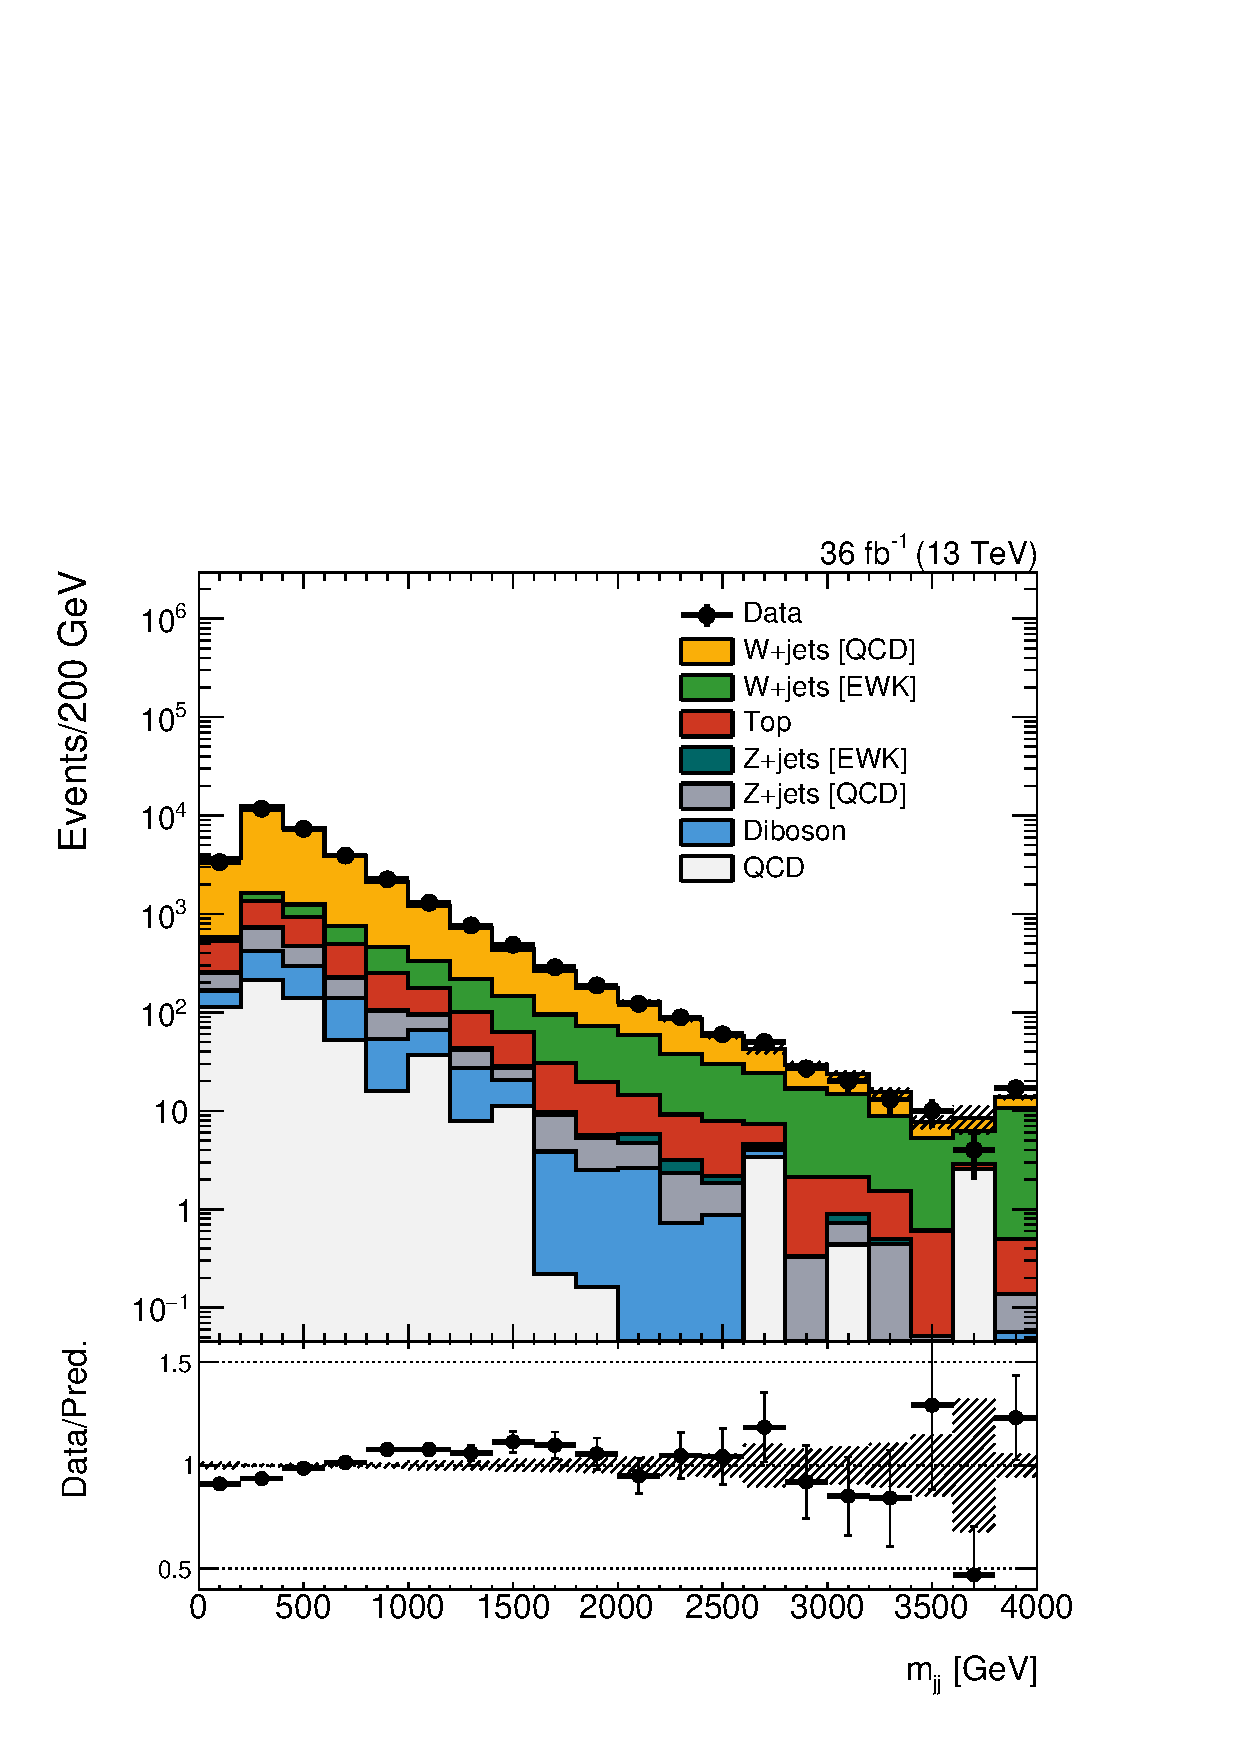
\includegraphics[width=\textwidth]{figures/vbf/prefit/singlemuon_jot12Mass_logy.pdf}
        \end{subfigure}
        \begin{subfigure}[t]{0.24\textwidth}
            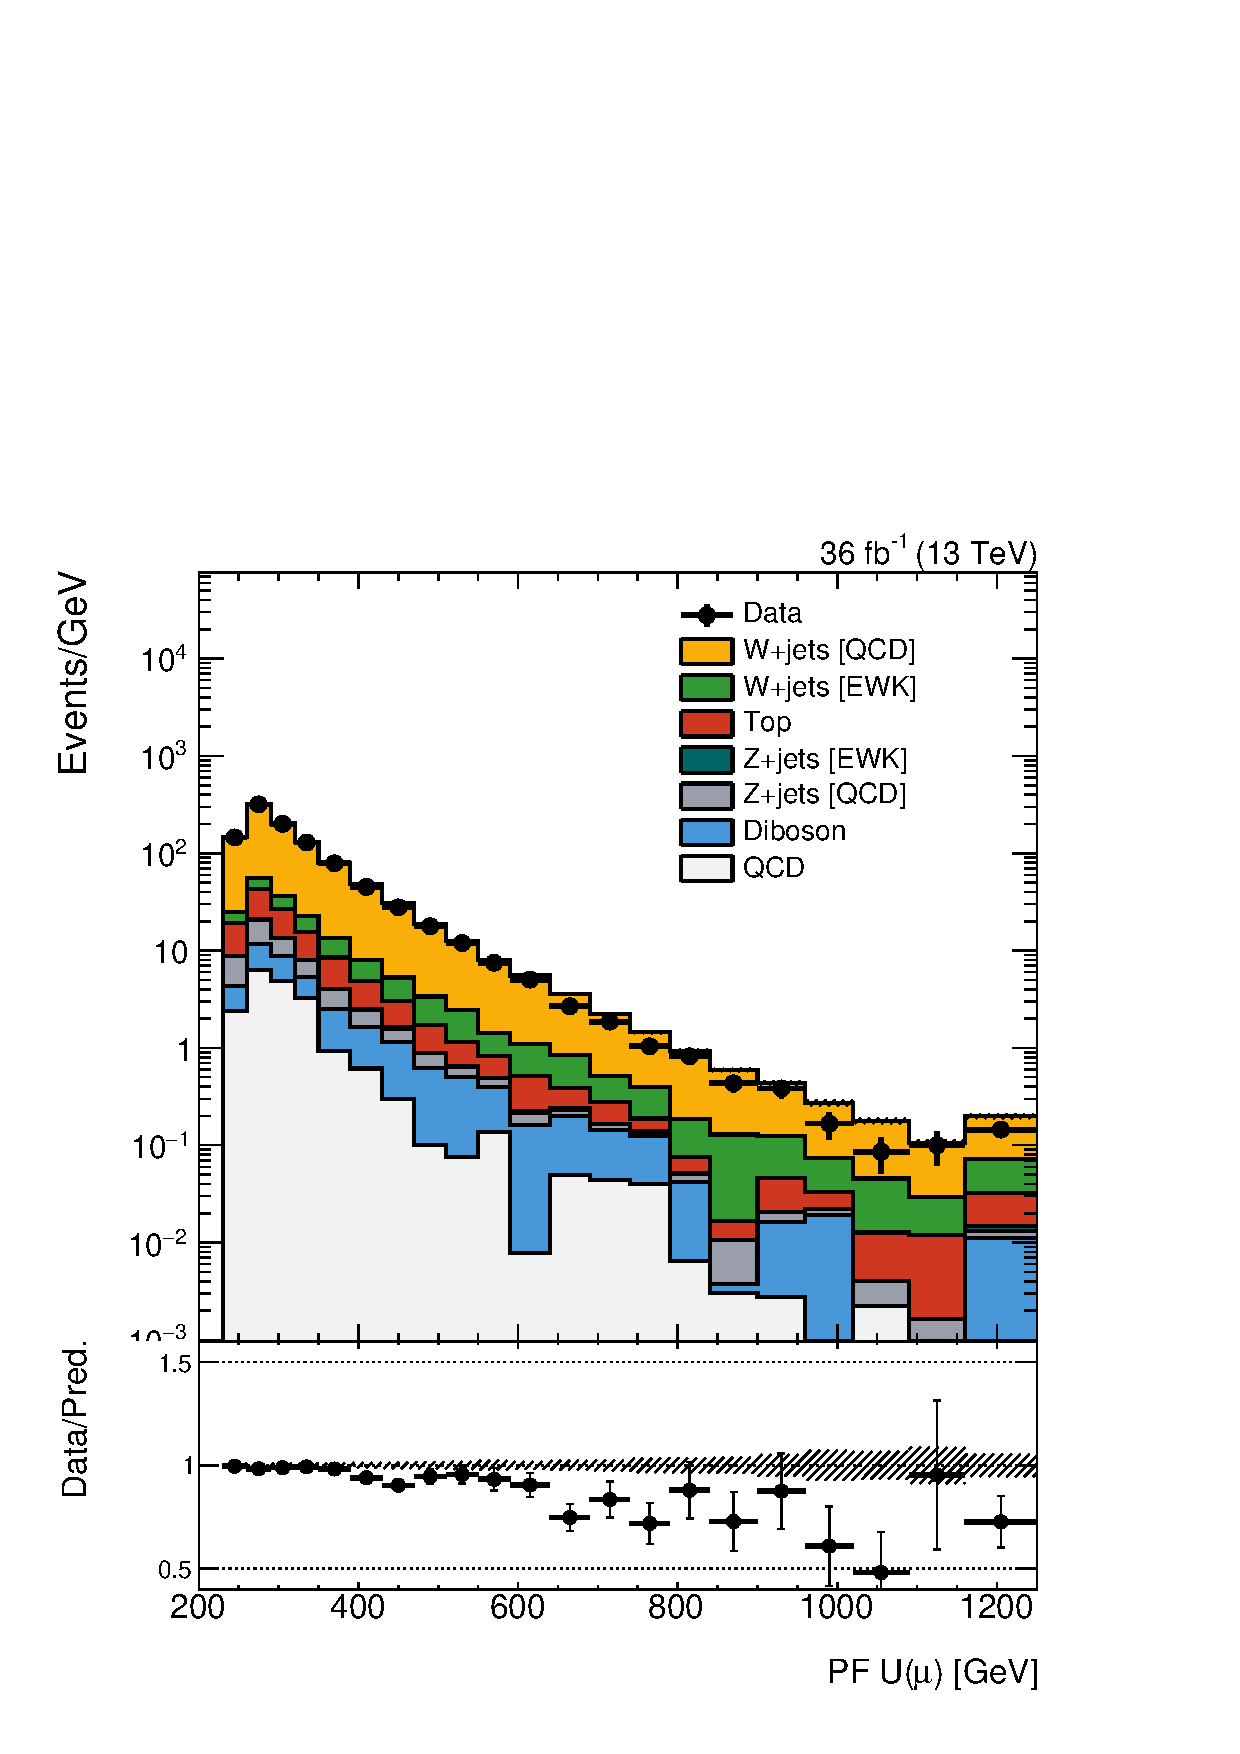
\includegraphics[width=\textwidth]{figures/vbf/prefit/singlemuon_pfUWmag_logy.pdf}
        \end{subfigure}
        \caption{Dijet and recoil distributions in the single-electron (top) and single-muon (bottom) CRs.}
        \label{fig:vbf:wcr}
    \end{center}
\end{figure}


\begin{figure}[]
    \begin{center}
        \begin{subfigure}[t]{0.32\textwidth}
            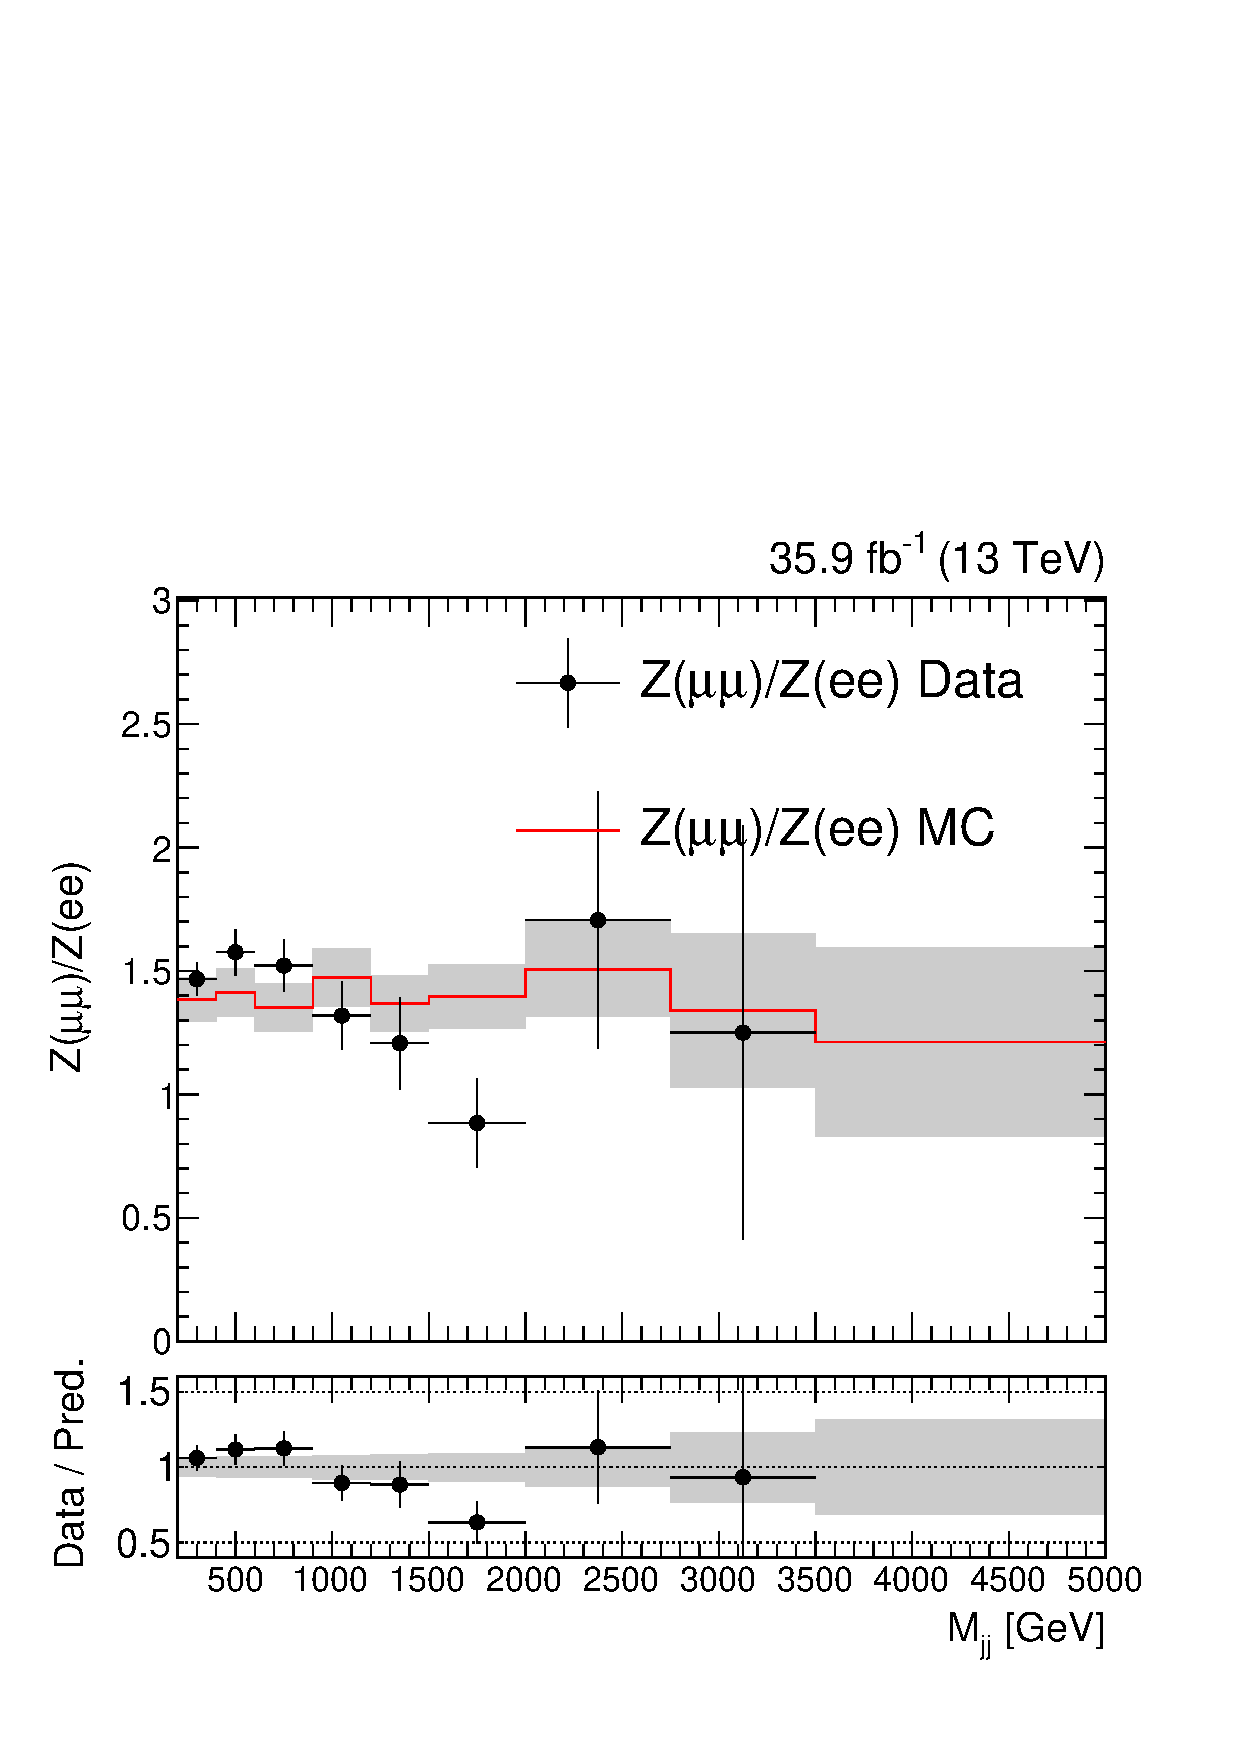
\includegraphics[width=\textwidth]{figures/vbf/fits/dimuon_dielectron_cat_vbf_ratio.pdf}
        \end{subfigure}
        \begin{subfigure}[t]{0.32\textwidth}
            \includegraphics[width=\textwidth]{figures/vbf/fits/singlemuon_singleelectron_cat_vbf_ratio.pdf}
        \end{subfigure}
        \begin{subfigure}[t]{0.32\textwidth}
            \includegraphics[width=\textwidth]{figures/vbf/fits/combined_combinedW_cat_vbf_ratio.pdf}
        \end{subfigure}
        \caption{Validation of the VBF transfer factors using control region data. 
                 The transfer factor proxies are found to agree quite well with the data within the post-fit uncertainties}
        \label{fig:vbf:valid}
    \end{center}
\end{figure}


\section{Results}

The dijet mass distribution in data is fit in all signal and control regions, the results of which are shown in Figure~\ref{fig:vbf:postfit}.
As no statistically significant excess over the Standard Model is observed, we translate the results into upper limits on the branching ratio of $\hinv$.
As the signal hypothesis, both the VBF and gluon fusion Higgs production modes are considered; the latter contaminates the SR due to its relatively large cross section.
After the signal region selection criteria, the two modes contribute approximately equal yields. 
Assuming $m_H=125$ GeV, the observed 95\% CL upper limit is 0.33. 
Assuming a background-only hypothesis, the expected distribution of upper limits has median $0.33$, with the 1 standard deviation band covering $[0.18,0.35]$; the observation therefore represents an upwards fluctuation slightly under $1\sigma$. 

\begin{figure}[]
    \begin{center}
        \begin{subfigure}[t]{0.32\textwidth}
            \includegraphics[width=\textwidth]{figures/vbf/fits/vbf_PULLS_prefit_postfit_signal.pdf}
            \caption{SR}
        \end{subfigure}
        \begin{subfigure}[t]{0.32\textwidth}
            \includegraphics[width=\textwidth]{figures/vbf/fits/vbf_PULLS_prefit_postfit_dimuon.pdf}
            \caption{$\mu\mu$ CR}
        \end{subfigure}
        \begin{subfigure}[t]{0.32\textwidth}
            \includegraphics[width=\textwidth]{figures/vbf/fits/vbf_PULLS_prefit_postfit_dielectron.pdf}
            \caption{$ee$ CR}
        \end{subfigure} \\ 
        \begin{subfigure}[t]{0.32\textwidth}
            \includegraphics[width=\textwidth]{figures/vbf/fits/vbf_PULLS_prefit_postfit_singlemuon.pdf}
            \caption{$\mu$ CR}
        \end{subfigure}
        \begin{subfigure}[t]{0.32\textwidth}
            \includegraphics[width=\textwidth]{figures/vbf/fits/vbf_PULLS_prefit_postfit_singleelectron.pdf}
            \caption{$e$ CR}
        \end{subfigure}
        \caption{Post-fit $m_{jj}$ distributions in the various signal and control regions.
                 The uncertainties (gray bands) and bin pulls (blue bands) are defined by varying the nuisances by one standard deviation around the maximum likelihood estimate.}
        \label{fig:vbf:postfit}
    \end{center}
\end{figure}

We further scan $m_H$ and set upper limits on $\sigma(qq\rightarrow qqH)\mathcal{B}(\hinv)$. 
In this case, as this is no longer the observed (Standard Model-like) Higgs boson, we only consider the VBF production mode as a signal hypothesis. 
The upper limits are shown in

\begin{figure}[]
    \begin{center}
        \includegraphics[width=0.5\textwidth]{figures/vbf/fits/mhscan.pdf}
        \caption{Upper limits on $\sigma\times \mathcal{B}$ as a function of $m_H$, assuming VBF as the only production mode.
                 The predicted cross section is shown in red.}
        \label{fig:vbf:mhscan}
    \end{center}
\end{figure}
